\chapter{Search for Supersymmetry and dark matter in events with dileptons and missing energy}
\label{sec:CandCanalysis}

%Beskriv prosessene her istedet for i teori og motiver hvordan partiklene er produsert. 

In this chapter we will introduce the processes we are searching for in the analysis, how the signal and background samples are produced and in the end how we do a traditional analysis. We will also show the results obtained by the ATLAS collaboration and compare the results with ours. 



The processes we are interested in looking at in this thesis involve superpartners of leptons, gauge bosons, and the Higgs boson. Besides this, we will look at a dark matter particle candidate, which is predicted to be the lightest supersymmetric particle (LSP).  This thesis looks at proton-proton collisions with final state two leptons and missing transverse energy (MET/$E_T^{miss}$). The SUSY processes we are looking at are direct slepton production, chargino production with slepton/sneutrino-mediated-decays and with W-boson-mediated-decays. 


In figure \ref{fig:SlepSlepFeynman} below, we can see the direct slepton production as a production of two hypothetical sleptons which decay to the final state, comprising of two leptons and missing transverse energy (i.e. missing energy in the detector). The neutralinos, which are the MET in this process, are a mixture of the sparticles photino, zino, and higgsino and is also one of the dark matter candidates mentioned above.  
\begin{figure}[H]
    \centering
    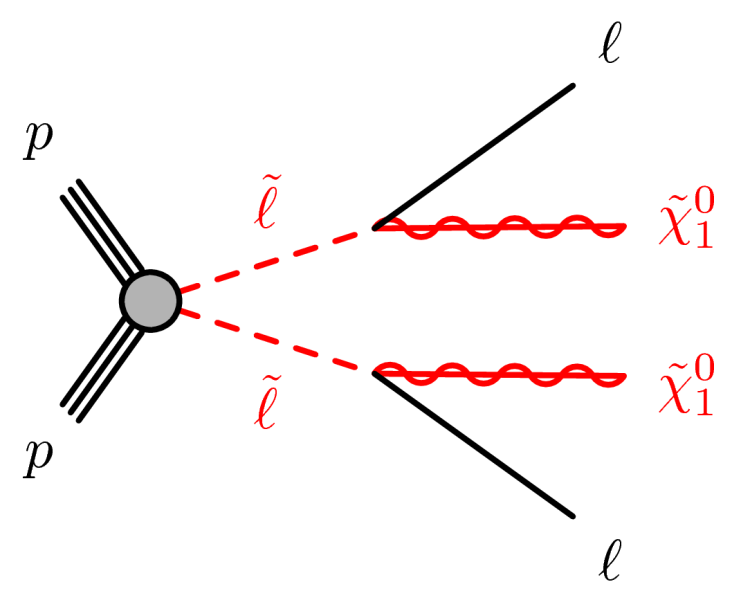
\includegraphics[width = 0.4\textwidth]{Figures/FeynmanDiagrams/SlepSlepFeynman.png}
    \caption{Direct slepton production $pp \rightarrow \tilde{l}^+ \tilde{l}^- \rightarrow l^+l^- + \tilde{\chi}_1^0 \tilde{\chi}_1^0$.}
    \label{fig:SlepSlepFeynman}
\end{figure}

In figure \ref{fig:SlepSnuFeynman} and \ref{fig:WWFeynman} we can see the chargino production with  slepton/sneutrino-mediated-decays and with W-boson-mediated-decays. Charginos are a mixture of the sparticles wino and the charged higgsino. These processes have the same final state as direct slepton production, but here the neutrinos are also a part of the MET, since we can't actually detect them in the detector. 
\begin{figure}[H]
    \centering
    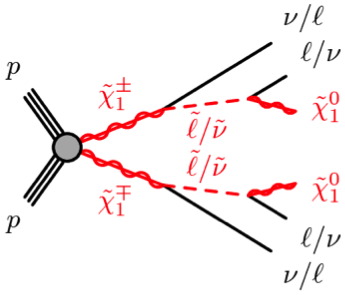
\includegraphics[width = 0.4\textwidth]{Figures/FeynmanDiagrams/SlepSnuFeynman.png}
    \caption{Chargino production with slepton/sneutrino-mediated-decays $pp \rightarrow \tilde{\chi}_1^+ \tilde{\chi}_1^- \rightarrow \tilde{l}^+ \tilde{l}^- /\tilde{\nu} \tilde{\nu} \rightarrow l^+l^- + \nu \Bar{\nu} + \tilde{\chi}_1^0 \tilde{\chi}_1^0$.}
    \label{fig:SlepSnuFeynman}
\end{figure}

\begin{figure}[H]
    \centering
    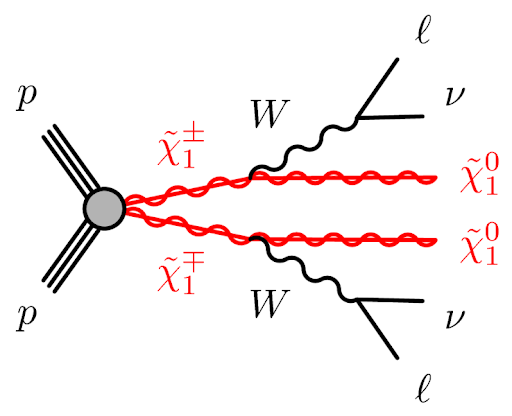
\includegraphics[width = 0.4\textwidth]{Figures/FeynmanDiagrams/WWFeynman.png}
    \caption{Chargino production with W-boson-mediated-decays $pp \rightarrow \tilde{\chi}_1^+ \tilde{\chi}_1^- \rightarrow W^+ W^- \rightarrow l^+l^- + \nu \Bar{\nu} + \tilde{\chi}_1^0 \tilde{\chi}_1^0$.}
    \label{fig:WWFeynman}
\end{figure}

The DM process we are looking at in this thesis is the mono-Z process shown in figure \ref{fig:monoZFeynman2}. Here we have a mediator V which decays into the DM particles $\chi$ and a W/Z that decays into two leptons. This gives us the same final state as we had for the SUSY processes.  

\begin{figure}[H]
    \centering
    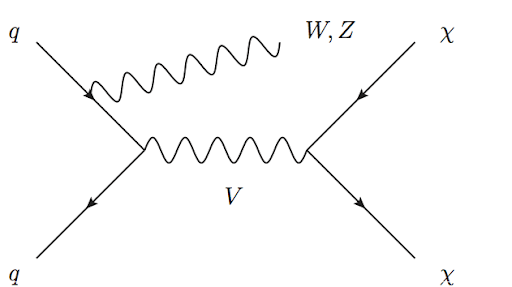
\includegraphics[width = 0.4\textwidth]{Figures/FeynmanDiagrams/monoZFeynman2.png}
    \caption{Mono-Z process $pp \rightarrow Z + MET \rightarrow l^+ l^- + MET$.}
    \label{fig:monoZFeynman2}
\end{figure}


\section{MC simulated events}

The data taken into consideration is from the ATLAS experiment at LHC between 2015-2018 (Run 2), further explained in chapter \ref{sec:LHCandATLAS}. But, we are also looking at some MC simulated background and signal which will be explained in this section. The explanations are taken from the publications from ATLAS, namely \cite{sleptonexclusion} for the SUSY signals and \cite{monoZexclusion} for the mono-Z signal. We present an overview of what signal samples that are used in table \ref{tab:directslepLOW} - \ref{tab:MonoZHigh} in section \ref{sec:sigsamptab}. 

The SUSY signal samples were generated from leading-order (LO) matrix elements with up to two extra partons using \textsc{MadGraph5\_aMC@NLO 2.6.1} \cite{48} interfaced to \textsc{Pythia 8.186} \cite{49}, with the A14 tune \cite{50}, for the modelling of the SUSY decay chain, parton showering, hadronisation and the description of the underlying event. Parton luminosities were provided by the NNPDF2.3LO PDF set \cite{51}. Jet–parton matching was performed following the CKKW-L prescription \cite{52}, with a matching scale set to one quarter of the mass of the pair-produced SUSY particles. Signal cross-sections were calculated to next-to-leading order (NLO) in $\alpha_s$ adding the resummation of soft gluon emission at next-to-leading-logarithm accuracy(NLO+NLL) \cite{53,54,55,56,57,58,59}. The nominal cross-sections and their uncertainties were taken from an envelope of cross-section predictions using different PDF sets and factorisation and renormalisation scales, as described in Ref. \cite{60}. 


To study the invisible Higgs boson decays, Monte Carlo events are produced for the SM ZH process with a subsequent Z boson decay into a dilepton pair and the H$\rightarrow$ZZ$\rightarrow \nu \nu \nu \nu$ decay (ZH$\rightarrow ll$+inv). The ZH signal processes from both the quark–antiquark (qqZH) and gluon–gluon (ggZH) initial states are modelled with \textsc{Powheg-Box v2} \cite{49Z, 50Z} using the CT10 \cite{51Z} parton distribution function (PDF) and interfaced to \textsc{Pythia8.186} \cite{52Z} for parton showering. The kinematic distributions of ZH$\rightarrow ll$ +inv events are described at next-to-leading-order (NLO) in QCD. Additionally, for the qqZH process, the MINLO \cite{53Z} method is applied to improve the gluon resummation calculation, and the $p_T^Z$ distribution is corrected to NLO electroweak (EW) accuracy with a reweighting approach detailed in Ref. \cite{3Z}. The SM ZH production cross-section is computed with next-to-next-to-leading-order (NNLO) QCD and NLO EW precision and found to be 884 fb \cite{3Z} with $m_H = 125$ GeV at 13 TeV. The DM signal is modelled with the leading-order \textsc{MadGraph5\_aMC@NLO} matrix element \cite{54Z} using NNPDF3.0 \cite{55Z} and showered with Pythia8.186. DM signal events with an axial-vector mediator and fermionic WIMPs are produced for different $m_{med}$ and $m_\chi$, both in a range from 10 to 1000 GeV.  As recommended in Ref. \cite{44Z}, the DM events are generated by choosing $g_q = 0.25$, $g_\chi = 1$, and a minimal mediator width. The AZNLO \cite{56Z} and A14 \cite{57Z} parameter sets are used to tune the \textsc{Pythia8.186} parton-shower for the simulation of the ZH $\rightarrow ll$+inv and DM signals, respectively.


The different backgrounds that we are considering are diboson, triboson, $t\Bar{t}$, single top, other top events ($t\Bar{t}$ events with a pair of leptons or boson(s)), Higgs, Drell-Yan, Z+jets and W+jets. The MC samples are simulated using different generators that are listed up in table \ref{tab:bkg_samples}. The goal is to separate these backgrounds from the signals we are looking at, which consist in the four different processes that we looked at earlier in this chapter. 

\begin{table}[H]
    \centering
    \begin{tabular}{l l l l} \toprule
        \textbf{Background sample} & \textbf{Generator} & \textbf{Parton shower} & \textbf{Normalisation}\\
        \midrule
        \midrule
        Diboson & \textsc{Sherpa2.2.2}\cite{sherpa2_1, sherpa1_2, sherpa1_3} & \textsc{Sherpa2.2.2} & NLO \cite{NLO}\\
        Triboson & \textsc{Sherpa2.2.2} & \textsc{Sherpa2.2.2} & NLO \\
        Z+jets & \textsc{Sherpa2.2.1} \cite{sherpa1_1, sherpa1_2, sherpa1_3} & \textsc{Sherpa2.2.1} & NNLO \cite{NNLO}\\
        W+jets & \textsc{Powheg-Box v2}\cite{49Z, 50Z} & \textsc{Pythia8.186} \cite{49} & NLO\\
        Drell-Yan & \textsc{Sherpa2.2.1} & \textsc{Sherpa2.2.1} & NNLO\\
        $t\Bar{t}$ & \textsc{Powheg-Box v2} & \textsc{Pythia8.186} & NNLO\\
        Single top & \textsc{Powheg-Box v2} & \textsc{Pythia8.186} & NLO\\
        topOther & \textsc{MG5\_aMC@NLO} \cite{48} & \textsc{Pythia8.186} & NLO\\
        Higgs & \textsc{Powheg-Box v2} & \textsc{Pyhtia8.186} & NLO\\
        \bottomrule
    \end{tabular}
    \caption{An overview of the different generators used to simulate the MC background samples.}
    \label{tab:bkg_samples}
\end{table}


Before we move on to how we perform the analysis, we also need to know how we are going to know that we see SUSY and DM particles in the detector. Since they never have been discovered, we have to lean on some hypotheses on how this is happening. As for all events in the detector, we have to reconstruct the events using their decays. The supersymmetric particles are expected to decay into cascades that will contain a LSP which will interact very weakly with the detector material which again will result in a big measured MET in the detector. The rest of the cascade will result in a final state with with leptons and/or jets. Together with the MET this gives us the final state we are looking for. For the mono-Z process we can measure the MET from the DM particles decayed from the unknown hypothetical mediator particle. Together with the leptons we get from the decay of the Z-boson, this gives us the same final state as for the SUSY processes.




































\begin{comment}

\begin{itemize}
    \item Bruker noe som eksisterer
    \item Tradisjonell måte ting har blitt gjort på
    \item begrenset av menneskets forståelse av prosessen vi ser på
    \item vi må bestemme alle kuttene som blir gjort
    \item Du må vite hva du skal se etter for å gjøre dette, altså trenger en teori/hypotese
    \item Tenk overgang til ML
    \item Valg må være begrunnet 
    \item Massesplitting. Cut and count er svak på lav massesplitting. Dette gjør ML bedre
\end{itemize}
\end{comment}








\section{The standard way: Cut and count}
\label{sec:candc}

The first part of the analysis done in this thesis is a traditional cut and count analysis. \textit{Cut and count} is probably the most known method used in particle physics and has proved to be very effective in the discoveries we have done so far. Since the data become more and more massive and the processes we are looking at more and more complicated, we also need to develop further the way we perform the analysis. In this thesis we are mainly going to focus on machine learning algorithms. Therefore I have not done much with this standard way to do an analysis and have used an already existing tool developed at CERN.  

In cut and count, we select events sensitive to new physics, i.e., we cut away events that are not interesting for the process we are considering according to some selection criteria. After applying one cut/selection, the events we are left with form the so-called called \textit{signal region}. We then see whether the signal is separated from our Standard Model (SM) background in this region. We can calculate an expected significance $Z$, which will be explained in section \ref{sec:significance} later in the thesis, to check if we can expect to claim any discovery in this region at all. If we are lucky and have cut away enough background to separate the signal from the background, we can also see if the events left in the data are compatible with the signal or if they keeps matching the background instead. Let us consider the case where the data differ from the background and tends to follow the signal: we know that there is most likely something interesting in this region.

Of course, there are advantages and disadvantages with every method, and this is also the case for cut and count. In cut and count, we need a theory or hypothesis as a reference, so we know what kind of signals we should look for. It is therefore unfortunately limited by the human understanding of what we are looking at. The lack of human understanding is where Machine Learning (ML) comes to help. The ML methods help us separate the signal from the background. This is further explained in the following chapters, where we will look at what the different ML methods do.



\begin{comment}
The analysis methods in high energy physics is constantly evolving and we have during the many years in this field looked in new directions to find better methods to use. The main method that have been used so far is the cut and count analysis which is presented in this chapter, but unfortunately this method is limited by the human understanding of the data. This is one of the reasons why we also have added ML to our analysis methods which will be presented in chapter \ref{sec:MLanalysis}.
\end{comment}

\section{Reproducing the ATLAS publications}
The first part of this analysis was done by cut and count and the goal was to reproduce the results from publications done by ATLAS. Here we will compare our results to the results obtained at the ATLAS experiment and hopefully we will get a good agreement between these two.

Since the goal is to reproduce the same results someone else have obtained, it is a good start to do the same analysis procedure as the publications. The cuts done for the SUSY processes are listed in table \ref{tab:cutsSUSY} and for the mono-Z process in table \ref{tab:cutsDM}, where both tables are taken from the publications. All the kinematic variables we do cuts on are presented in The first cut we do for both processes is to demand only two lepton with opposite sign in the final state.


\begin{table}[H]
    \centering
    \begin{tabular}{l l}\toprule
    \textbf{Variables} & \textbf{Cuts}\\
    \midrule
    \midrule
    Two leptons & Same flavor (SF) and opposite sign (OS)\\
    $n_{\text{non-b-tagged jets}}$     & 0 \\
    $m_{ll}$ [GeV]     & 121.2\\
    $E_T^{miss}$ [GeV] & $>$ 110 \\
    $E_T^{miss}$ significance & $>$ 10\\
    $n_{\text{b-tagged jets}}$ & 0\\
    $m_{T2}$ & 160\\
    \bottomrule
    \end{tabular}
    \caption{Cuts added in the cut and count analysis taken from the publication for the SUSY processes \cite{sleptonexclusion}.}
    \label{tab:cutsSUSY}
\end{table}

For the SUSY processes we have applied the cuts in table \ref{tab:cutsSUSY}, where we in addition to have only two leptons with opposite sign in the final state, we demand that they have to have the same flavor as well. It is done a cut on the missing transverse energy as well, even though this is something we want in our final state. This is done because this will cut away more background than signal which entails that we will obtain a bigger separation between the signal and background. We are also demanding to have no jets at all (both b-tagged and non-b-tagged jets). The last cuts we apply is a cut on the invariant mass of the two leptons in the final state and a cut on the stransverse mass for the two invisible particles in the final state. 

\begin{table}[H]
    \centering
    \begin{tabular}{l l}\toprule
    \textbf{Variables} & \textbf{Cuts}\\
    \midrule
    \midrule
    Two leptons     &  OS with leading (subleading) $p_T >$ 30 (20) GeV\\
    $m_{ll}$     & 76 $< m_{ll} <$ 106 GeV\\
    $E_T^{miss}$ & $>$ 90 GeV\\
    $E_T^{miss}/H_T$ & $>$ 0.6\\
    $\Delta \phi (\Vec{p}_T^{ll}, E_T^{miss})$ & $>$ 2.7 radians\\
    $\Delta R_{ll}$ & $<$ 1.8\\
    Fractional $p_T$ difference & $|p_T^{ll} - p_T^{miss, jets}|/p_T^{ll} <$ 0.2\\
    b-jets & 0\\
    \bottomrule
     \end{tabular}
    \caption{Cuts added in the cut and count analysis taken from the publication for the mono-Z process \cite{monoZexclusion}.}
    \label{tab:cutsDM}
\end{table}

For the DM process we have applied the cuts in table \ref{tab:cutsDM}, where we, as for the SUSY processes, demand to only have two leptons with opposite sign (but not necessary same flavor) in the final state together with missing transverse energy. In addition to the number of lepton cut, we do a cut on the $p_T$ of the leptons, where the leading lepton have a cut on 30 GeV and the subleading lepton have a cut on 20 GeV. We also do a slightly more gentle cut on the missing transverse energy for this process on 90 GeV, but we also have another variable that is depended on the missing transverse energy, namely $E_T^{miss}/H_T$ on 0.6. The next cut that is applied is $\Delta \phi (\Vec{p}_T^{ll}, E_T^{miss})$, where the two leptons also have to be close to each other which can be demand by $\Delta R_{ll}$. We do also a cut on the fractional $p_T$ difference and demand no b-tagged jets. 

All of the cuts are applied to get less background events while we at the same time do not want to cut away to much of the signal events. The publications have applied more or less the same cuts as listed above in table \ref{tab:cutsSUSY} and \ref{tab:cutsDM}, and their results are presented in figure \ref{fig:atlaspub}.


\begin{figure}[H]
\centering
    \begin{subfigure}[H]{0.49\textwidth}
        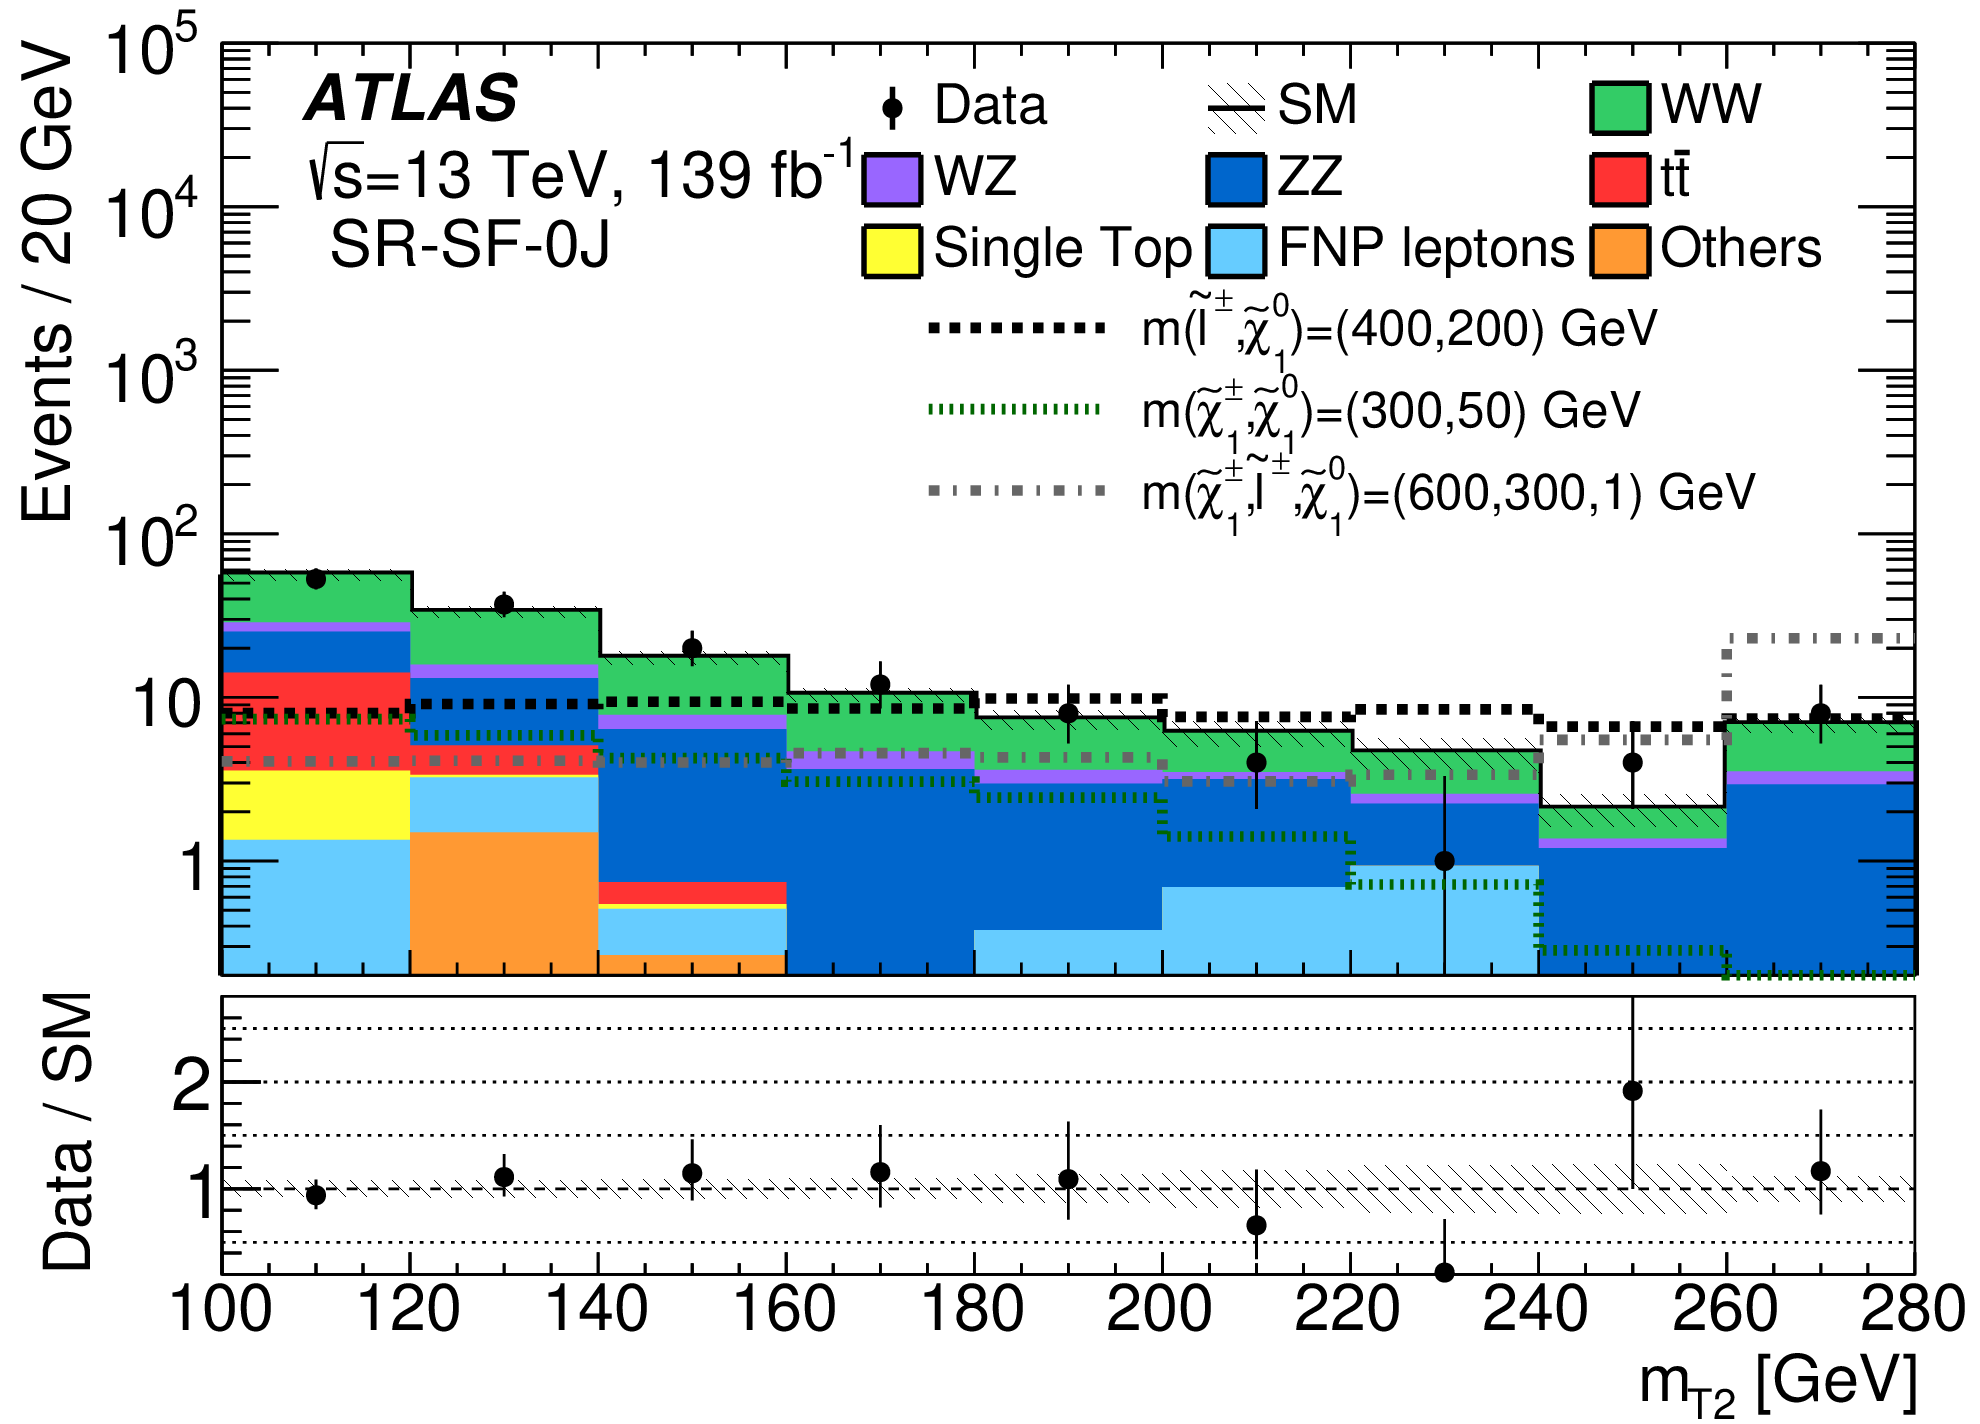
\includegraphics[width=\textwidth]{Figures/FromOnline/atlasmt2SUSY.png}
    \caption{Stransverse mass for direct slepton production, chargino production with $\Tilde{l}/\Tilde{\nu}$-mediated decays and with W-boson-mediated decays.}
    \label{fig:atlasSUSY}
    \end{subfigure}
    \\
    \begin{subfigure}[H]{\textwidth}
        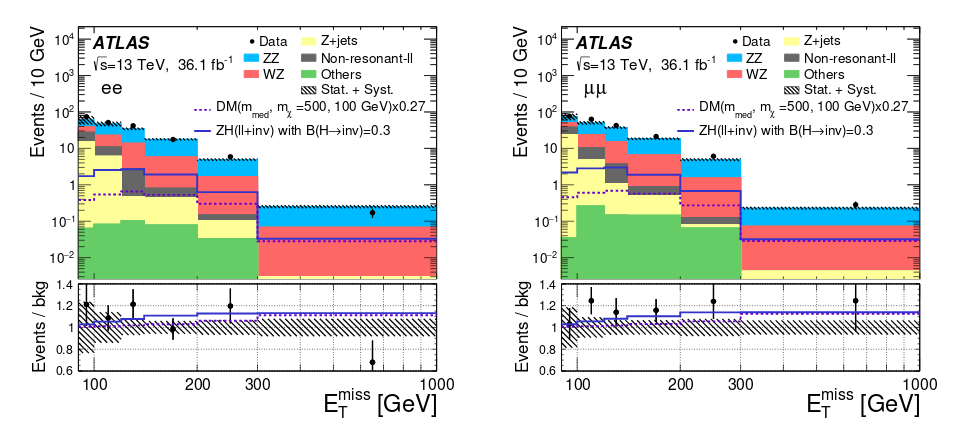
\includegraphics[width=\textwidth]{Figures/FromOnline/atlasmetDM.png}
    \caption{Missing transverse energy for the mono-Z process, where the left plot is the electron channel and right is the muon channel.}
    \label{fig:atlasDM}
    \end{subfigure}
    \caption{Results from the ATLAS publications for the four processes considered in this thesis.}
    \label{fig:atlaspub}
\end{figure}

In figure \ref{fig:atlasSUSY} we can see that the signal are separated from the background for both the direct slepton production and the chargino production with W-boson-mediated-decay, but not for chargino production with slepton/sneutrino-mediated-decay. Which means that we should not expect to claim any discovery for this mass splitting for the slepton/sneutrino-mediated-decay. 

In figure \ref{fig:atlasDM} we can see the plots for both electron channel and muon channel for the mono-Z process. It is not as much separation between signal and background as for the direct slepton production and for the chargino production with W-boson-mediated-decay.

Later in this thesis we are going to calculate the expected significance for the different processes we are looking at with both cut and count and ML. This is not done in the publication we are looking at, but they have included an exclusion plot where we can see where we expect to see some signal. This is shown in figure \ref{fig:exclusionPlots}. Here we can see the expected exclusion limit with $\pm1\sigma$ uncertainty bin together with t. We are not going to reproduce these results in this thesis, but we are going to use this to see what signals we have enough sensitivity to actually discover in the detector.

\begin{figure}[H]
    \centering
    \begin{subfigure}[t!]{0.49\textwidth}
        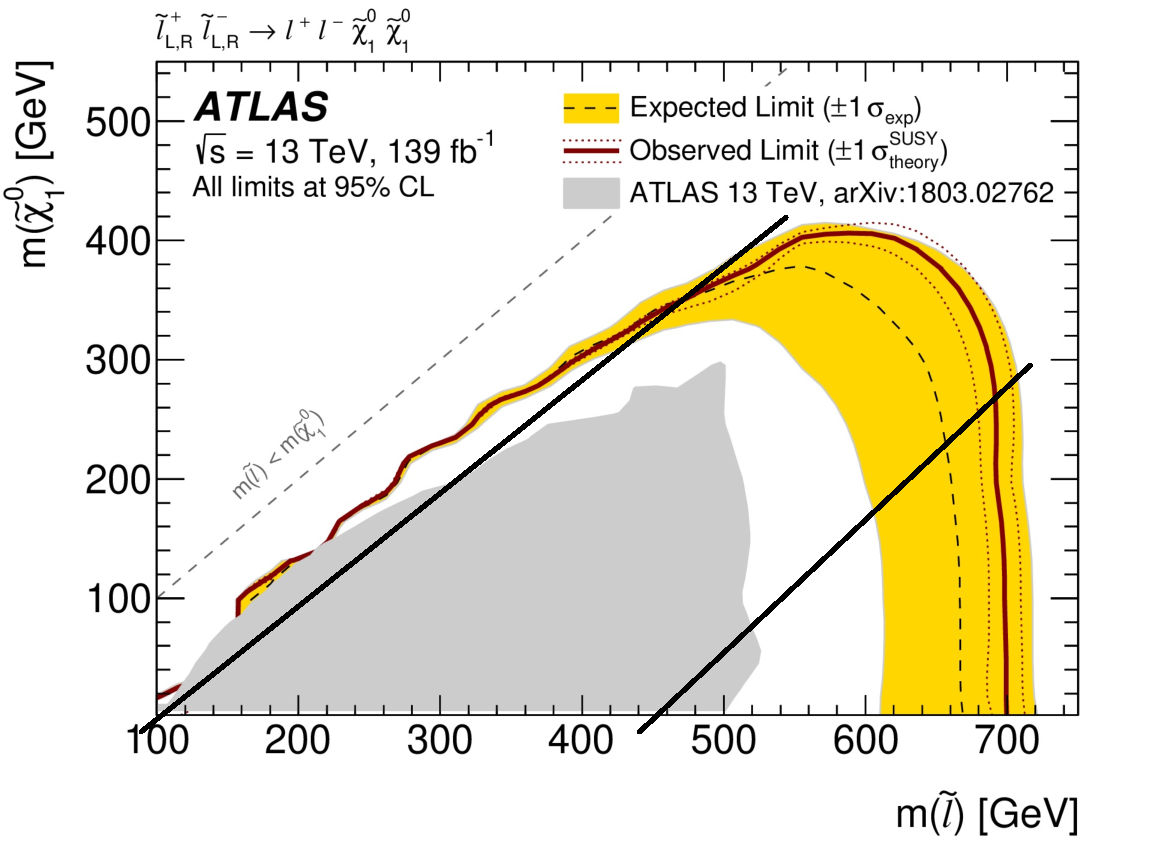
\includegraphics[width = \textwidth]{Figures/FromOnline/Slepslep.pdf}
        \caption{Slepton pair production ($\Tilde{l}\Tilde{l}$) \cite{sleptonexclusion}.}
        \label{fig:slepslepexclusion}
    \end{subfigure}
    \begin{subfigure}[t!]{0.49\textwidth}
        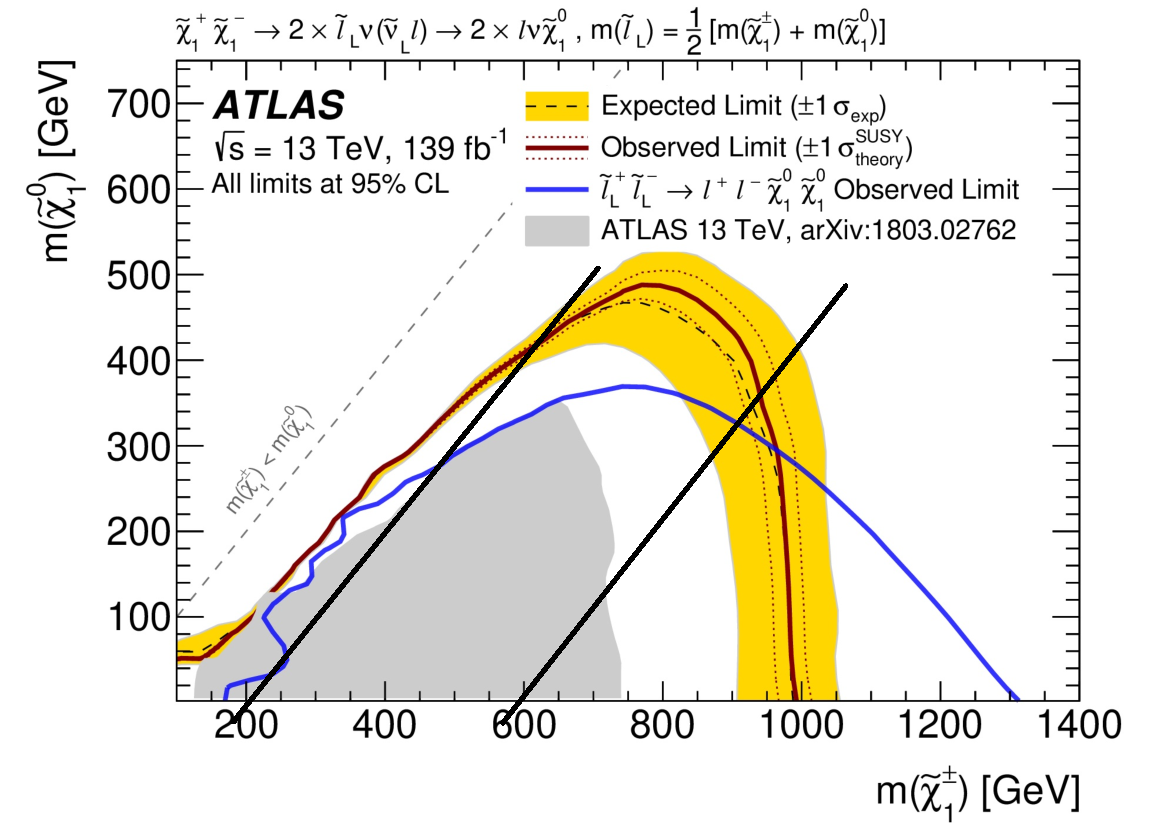
\includegraphics[width = \textwidth]{Figures/FromOnline/Slepsnu.pdf}
        \caption{$\chi_1^+ \chi_1^-$ production via $\Tilde{l}/\Tilde{\nu}$ \cite{sleptonexclusion}.}
        \label{fig:slepsnuexclusion}
    \end{subfigure}
    \\
    \begin{subfigure}[t!]{0.49\textwidth}
        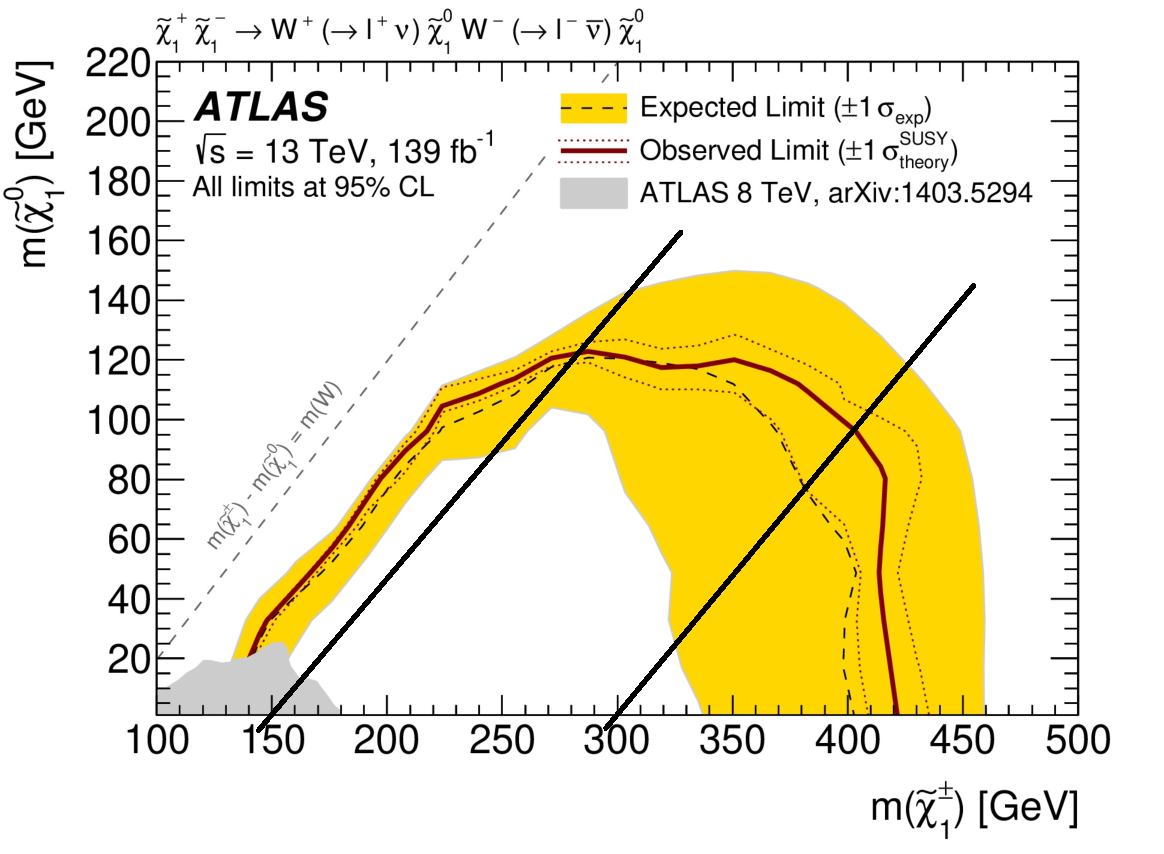
\includegraphics[width = \textwidth]{Figures/FromOnline/WW.pdf}
        \caption{$\chi_1^+ \chi_1^-$ production via W-boson \cite{sleptonexclusion}.}
        \label{fig:WWexclusion}
    \end{subfigure}
    \begin{subfigure}[t!]{0.49\textwidth}
        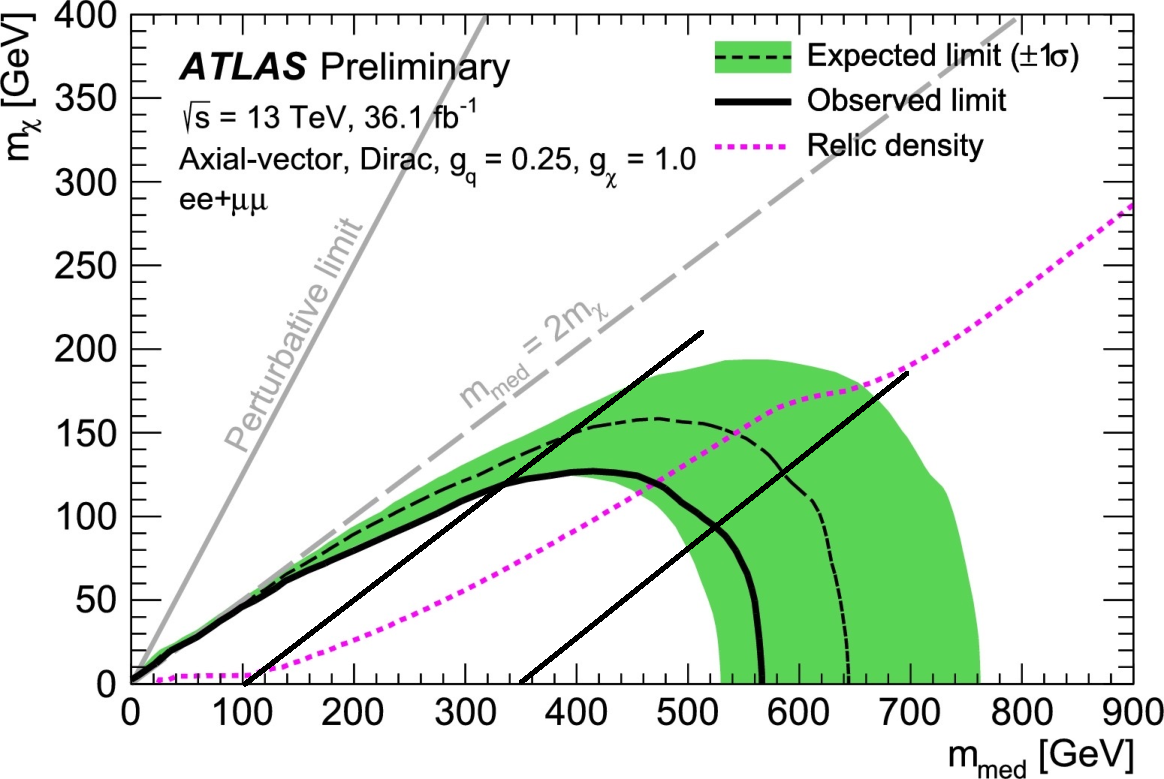
\includegraphics[width = \textwidth]{Figures/FromOnline/mono_Z.pdf}
        \caption{Mono-Z process \cite{monoZexclusion}.}
        \label{fig:monoZexclusion}
    \end{subfigure}
    \caption{The observed and expected exclusion limits for both the SUSY simplified models in \ref{fig:slepslepexclusion}, \ref{fig:slepsnuexclusion} and \ref{fig:WWexclusion} and for the DM model in \ref{fig:monoZexclusion}. The lines drawn in the plot is to show the mass splittings for each process.}
    \label{fig:exclusionPlots}
\end{figure}

If we look at figure \ref{fig:exclusionPlots}, we have drawn to black lines in each plot. This is done to split the signal samples into different mass splittings in the ML analysis later in the thesis. To have the opportunity to compare our ML results with the cut and count analysis, we have chosen one signal sample from each part of the plots in figure \ref{fig:exclusionPlots}. This gives us the signal samples listed up in table \ref{tab:sigsampcutandcount}.
\begin{table}[H]
    \centering
    \begin{tabular}{c c c c}
    \toprule
    $\mathbf{(\Tilde{l}, \Tilde{\chi}_1^0)}$ & $\mathbf{(\Tilde{\chi}_1^\pm, \Tilde{\chi}_1^0)}$ & $\mathbf{(\Tilde{\chi}_1^\pm, \Tilde{\chi}_1^0)}$ & $\mathbf{( V, \chi)}$  \\
    \midrule
    \midrule
    (400, 300) & (300, 200) & (150, 25) & (150, 80)\\
    (600, 300) & (800, 400) & (350, 100) & (400, 150)\\
    (700, 1) & (1000, 100) & (425, 25) & (650, 1)\\
    \bottomrule
    \end{tabular}
    \caption{An overview of what signal samples that are used for this thesis.}
    \label{tab:sigsampcutandcount}
\end{table}

These signal samples are going to follow us through both analysis (cut and count and ML). They are also shown in figure \ref{fig:cutandcountMONA} where we have followed the same procedure as the ATLAS publications. The main difference between the publications and our results is that we have chosen some other signal samples than the publications. The publications have $m(\Tilde{l}, \Tilde{\chi}_1^0) = (400, 200)$ GeV, $m(\Tilde{\chi}_1^\pm, \Tilde{\chi}_1^0) = (300, 50)$ GeV, $m(\Tilde{\chi}_1^\pm, \Tilde{\chi}_1^0) = (600, 300)$ GeV and $m(V, \chi) = (500,100)$ GeV. This makes it a bit hard for us to compare our results with the publication, but it is still doable. 


\newgeometry{twoside,inner=3cm,outer=2cm}
\begin{figure}[H]
%\begin{minipage}{2\textwidth}
%\begin{adjustwidth}{-3cm}{-3cm}
\centering
%\advance\leftskip-4cm 
%\advance\rightskip-4cm 
    \begin{subfigure}[t!]{0.49\textwidth}
        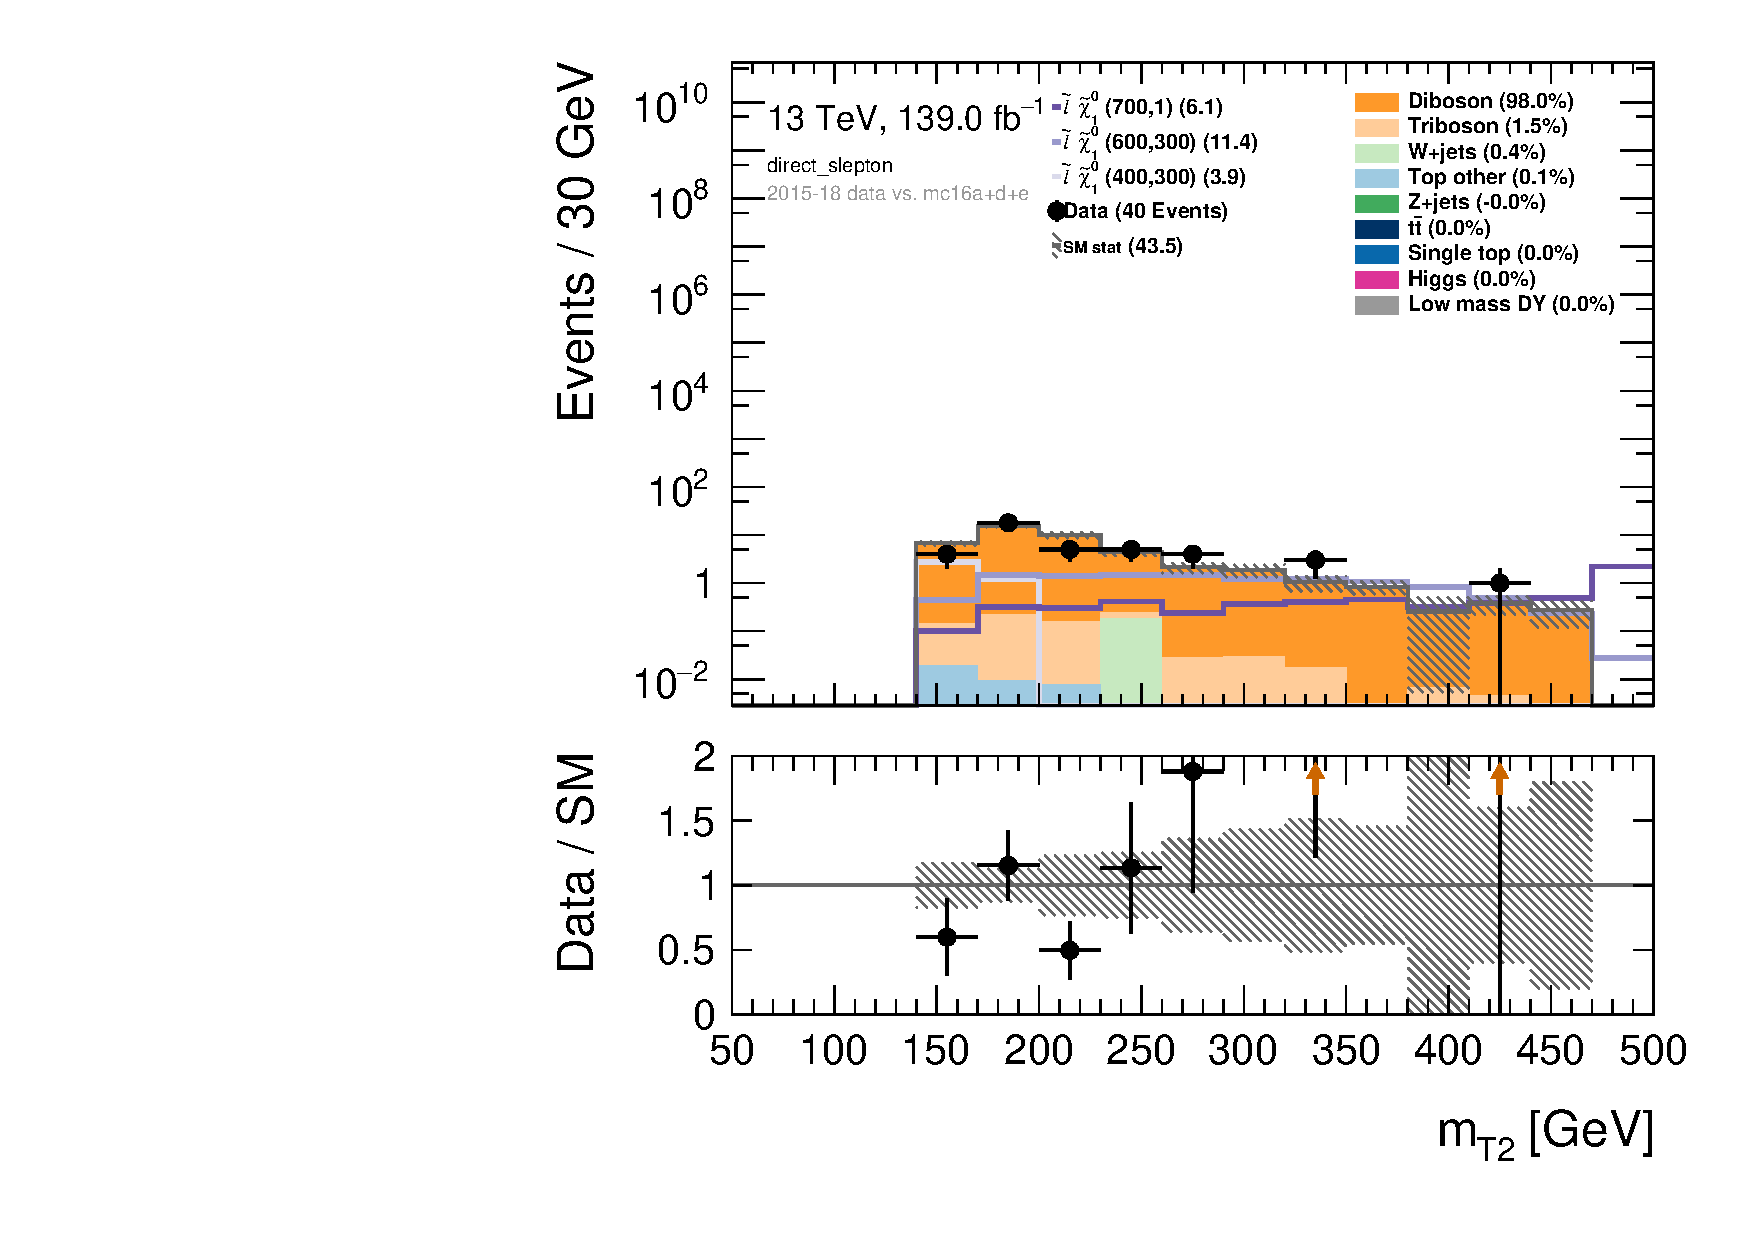
\includegraphics[width=\textwidth]{Figures/cutandcount/hist1d_mt2_direct_slepton.pdf}
    \caption{Stransverse mass for direct slepton production.}
    \label{fig:my_label}
    \end{subfigure}
    \begin{subfigure}[t!]{0.49\textwidth}
        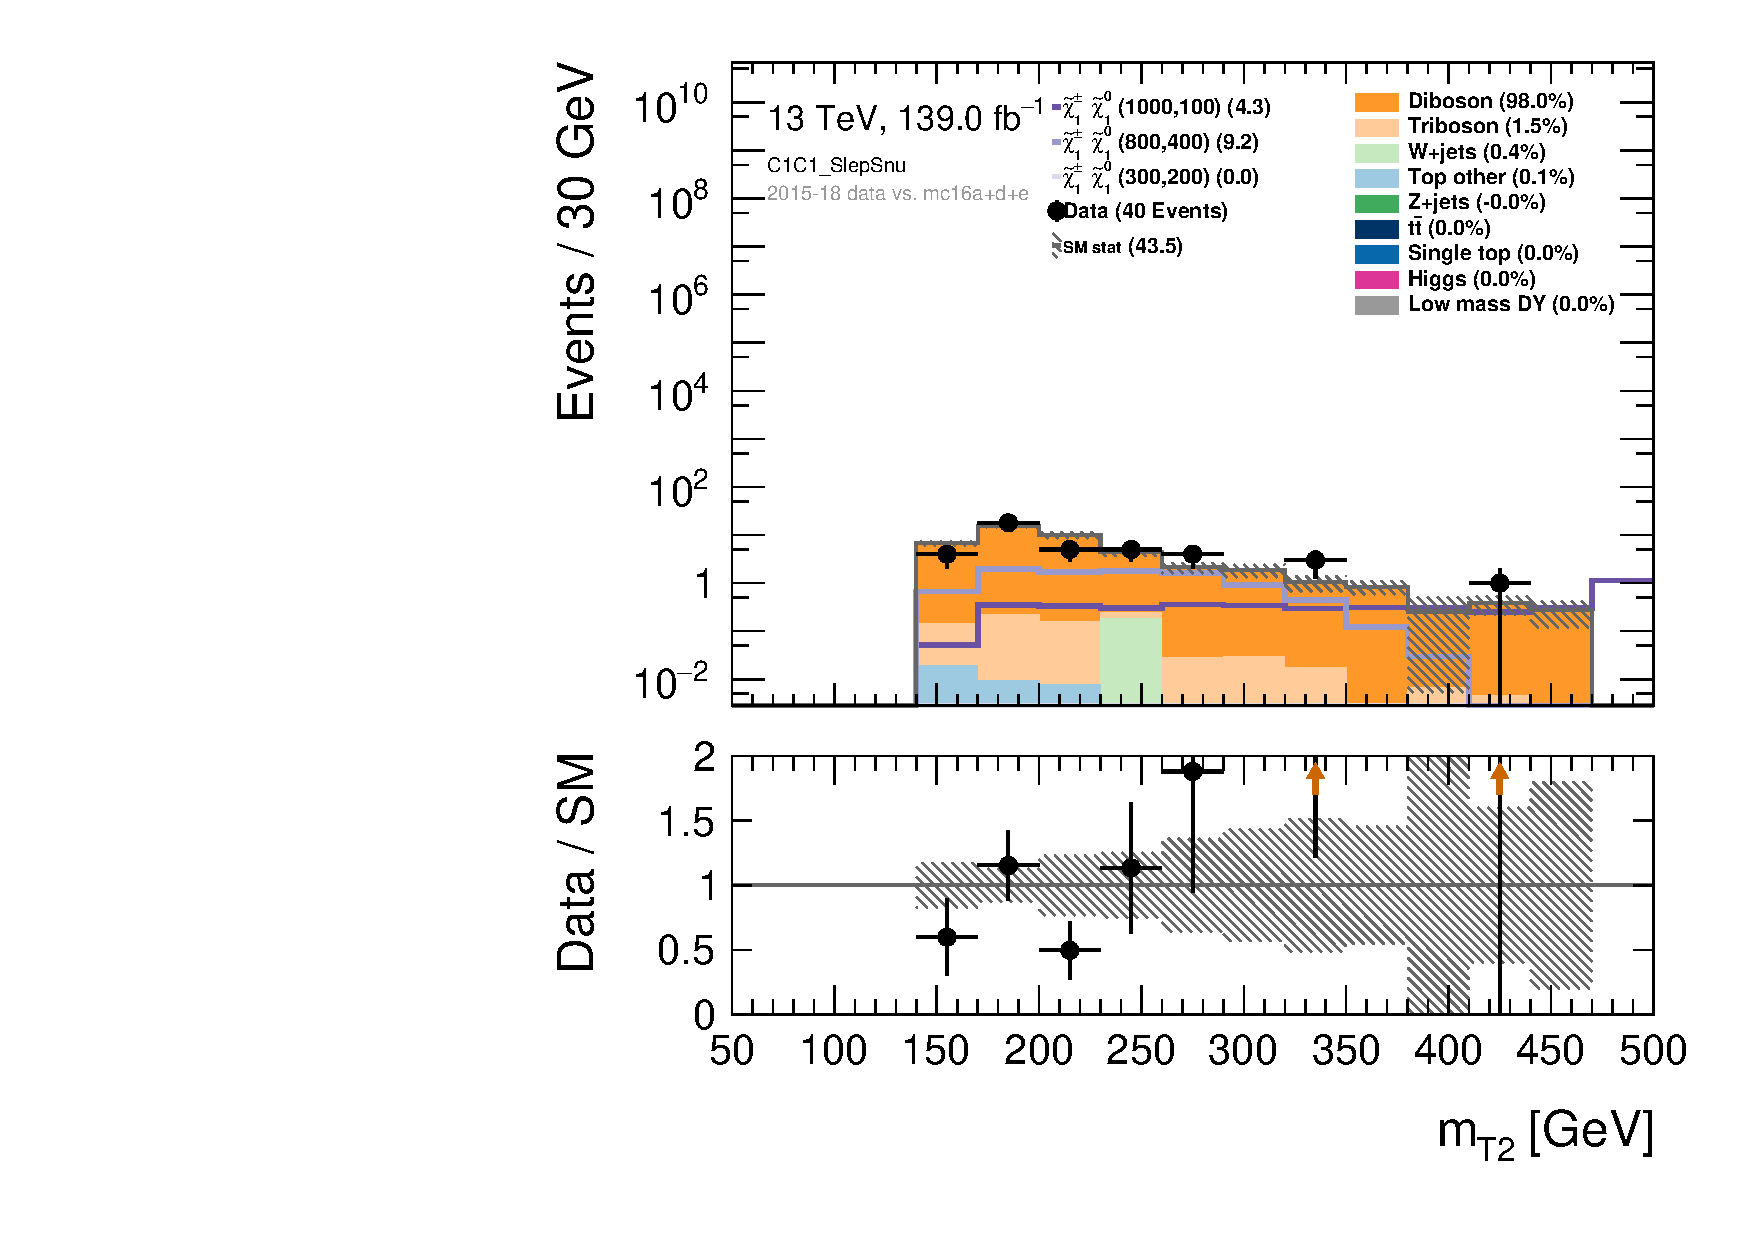
\includegraphics[width=\textwidth]{Figures/cutandcount/hist1d_mt2_C1C1_SlepSnu.pdf}
    \caption{Stransverse mass for chargino production via $\Tilde{l}/\Tilde{\nu}$.}
    \label{fig:my_label}
    \end{subfigure}
    \\
    \begin{subfigure}[t!]{0.49\textwidth}
        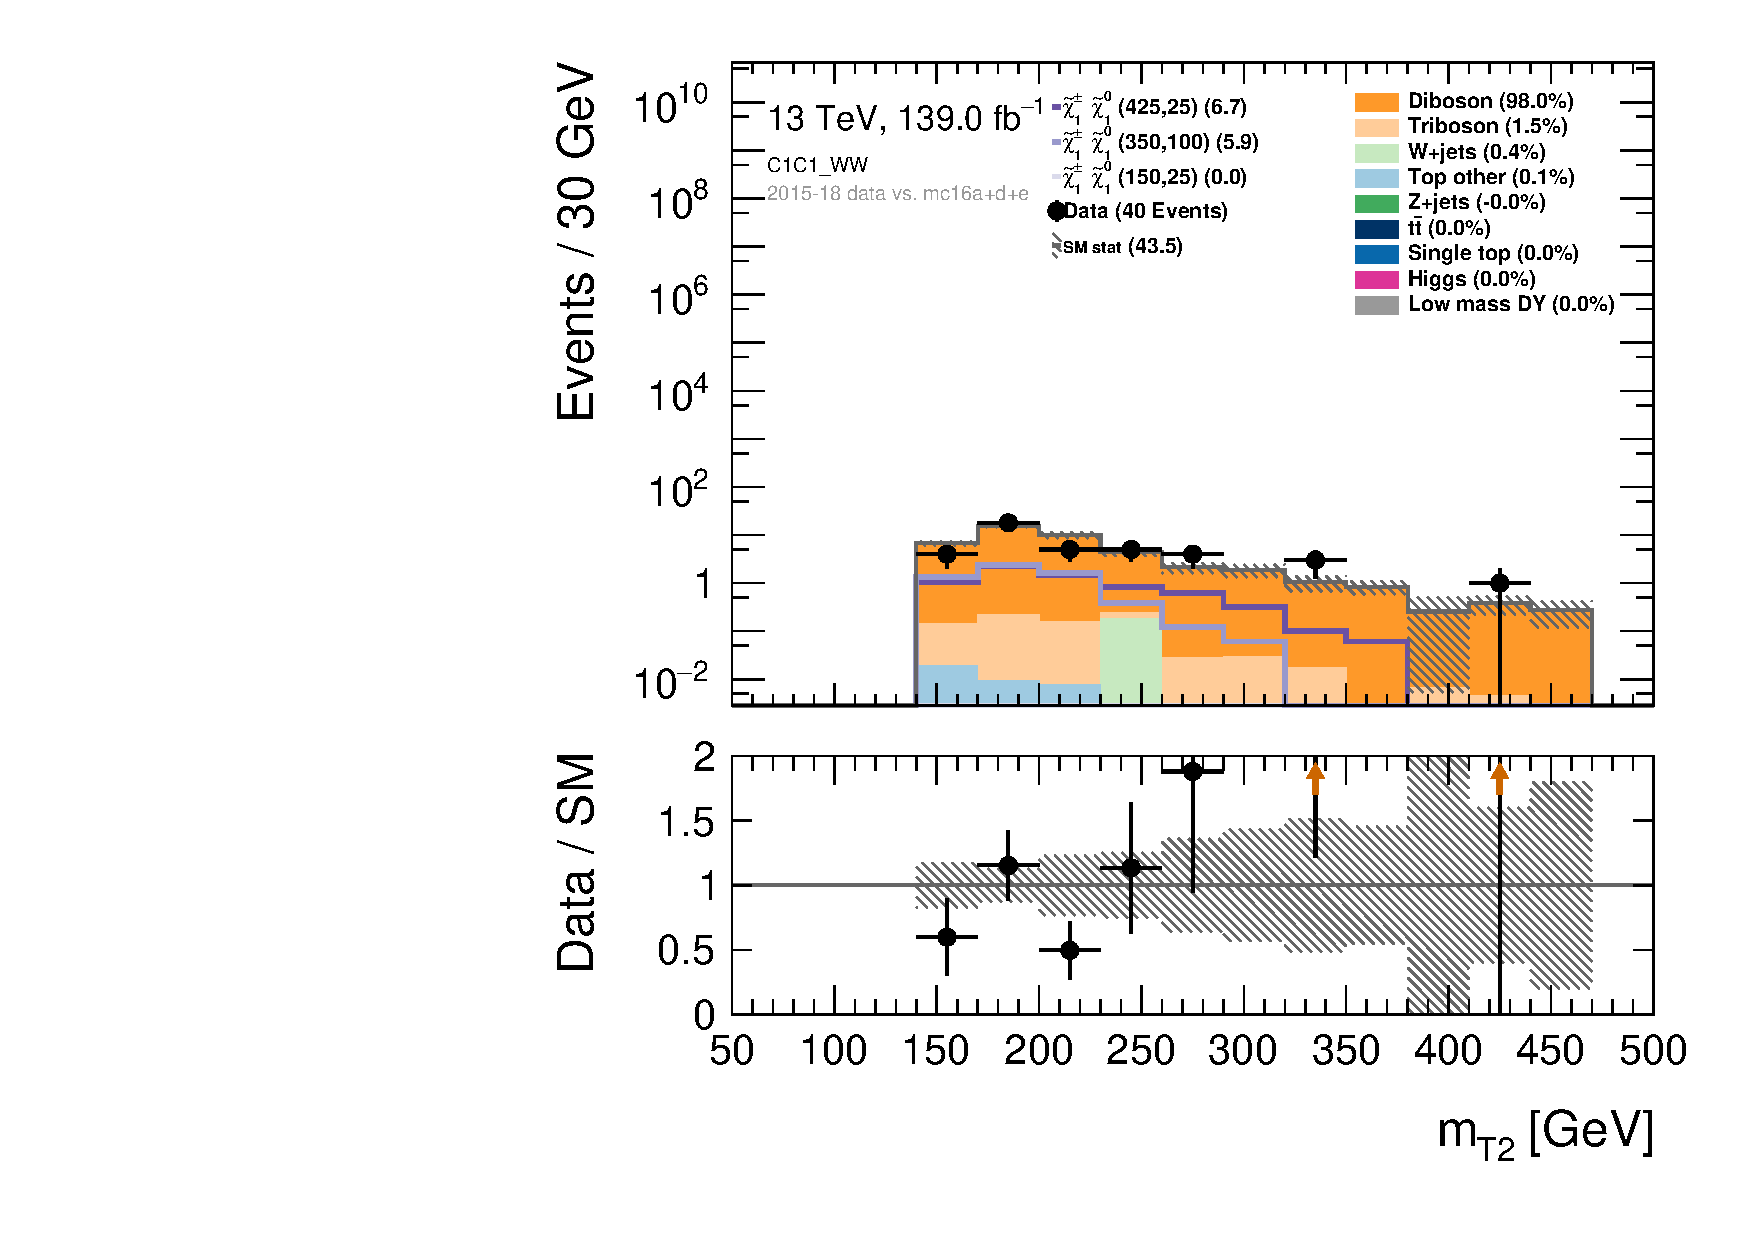
\includegraphics[width=\textwidth]{Figures/cutandcount/hist1d_mt2_C1C1_WW.pdf}
    \caption{Stransverse mass for chargino production via $W^\pm$.}
    \label{fig:my_label}
    \end{subfigure}
    \begin{subfigure}[t!]{0.49\textwidth}
        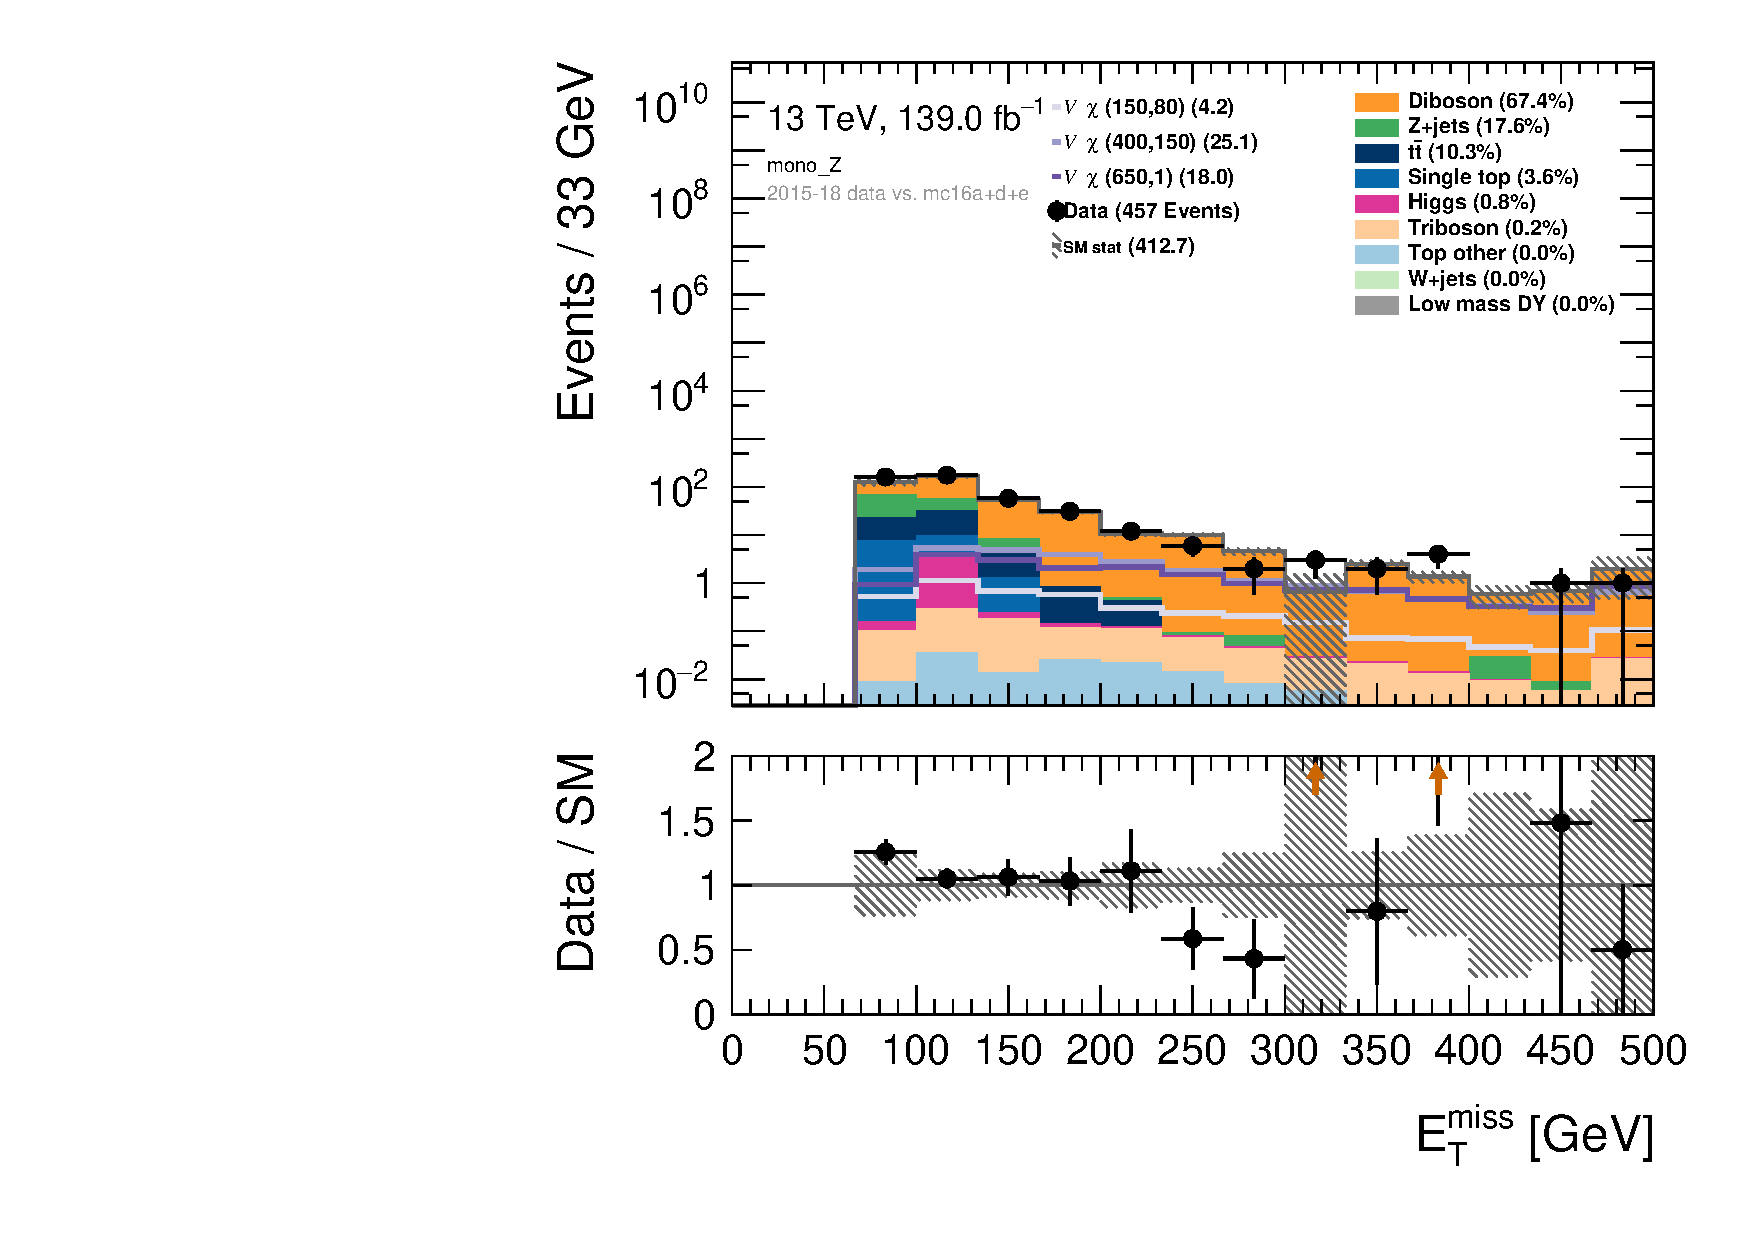
\includegraphics[width=\textwidth]{Figures/cutandcount/hist1d_met_Et_mono_Z.pdf}
    \caption{Missing transverse energy for mono-Z.}
    \label{fig:my_label}
    \end{subfigure}
    \caption{Plot of the four most important variables in direct slepton production with a cut on only two leptons with opposite charge in the final state.}
    \label{fig:cutandcountMONA}
\end{figure}
\restoregeometry

If we look at figure \ref{fig:cutandcountMONA} we can see that we have managed to separate the signal for both direct slepton production and chargino production with slepton/sneutrino-mediated-decay for the two signals with the highest mass splittings, and for the intermediate mass splitting for direct slepton production. 


\begin{comment}
%The first part of this analysis was done by cut and count. Here I have plotted four different variables which also represent some of the features used in the ML part. To demonstrate how the cut and count method behaves I have plotted each variable after adding a group of cuts. In the following figures you can see an example of this for the direct slepton production. You can also find examples of this for the charginos via slepton/sneutrino and via W-bosons in the appendix(OR GITHUB REPO??????). These two processes behave very similarly to the direct slepton production so I have chosen to show only one of them. 

%In the first figure \ref{fig:slepslep1stcut} we can see the whole mass distribution for the SM background with the final state two leptons with opposite charge. We can see that Z-jets is definitely the dominating background and by adding some cuts we can reduce this background.


\begin{figure}[H]
%\begin{minipage}{2\textwidth}
%\begin{adjustwidth}{-3cm}{-3cm}
\centering
%\advance\leftskip-4cm 
%\advance\rightskip-4cm 
    \begin{subfigure}[t!]{0.49\textwidth}
        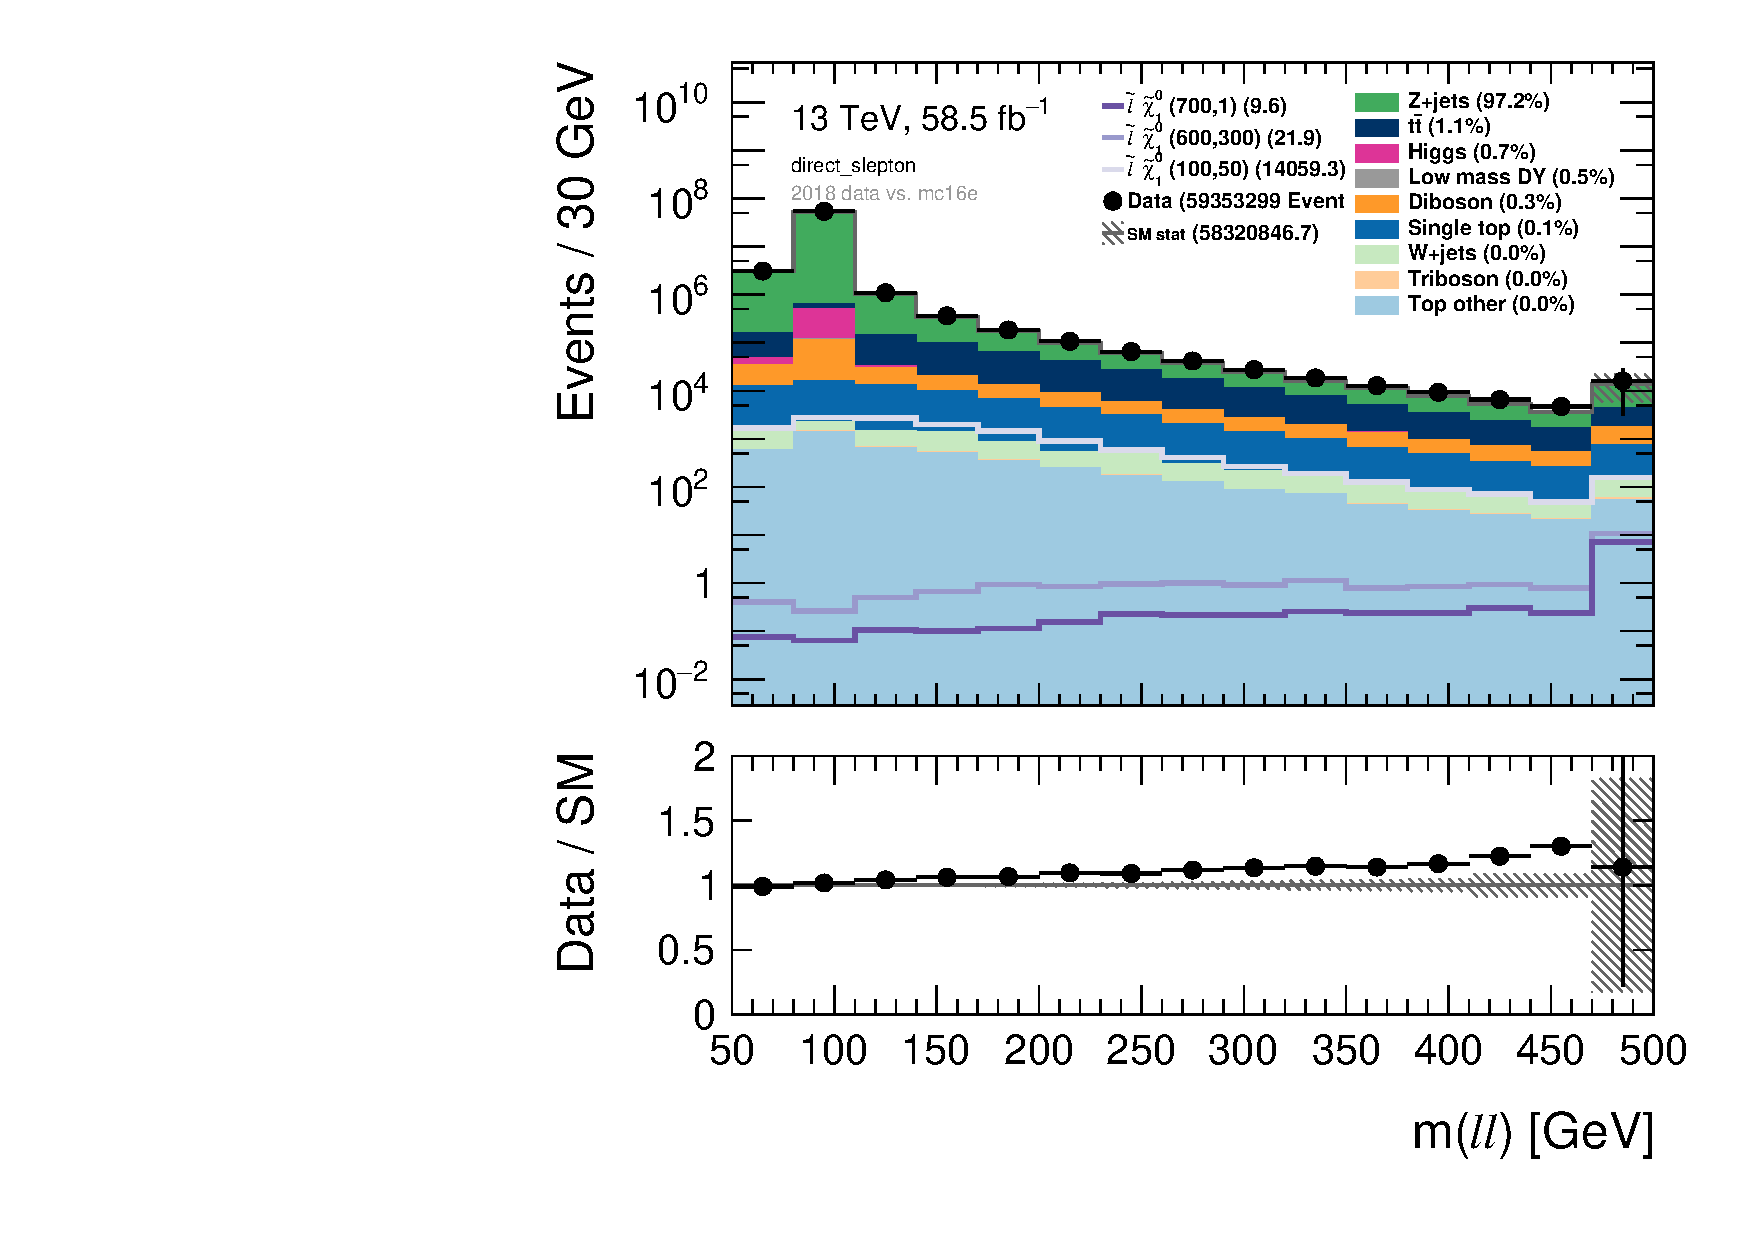
\includegraphics[width=\textwidth]{Figures/SlepSlep/CutAndCount/1stcut_2L+OS/hist1d_mll_direct_slepton.pdf}
    \caption{Invariant mass}
    \label{fig:my_label}
    \end{subfigure}
    \begin{subfigure}[t!]{0.49\textwidth}
        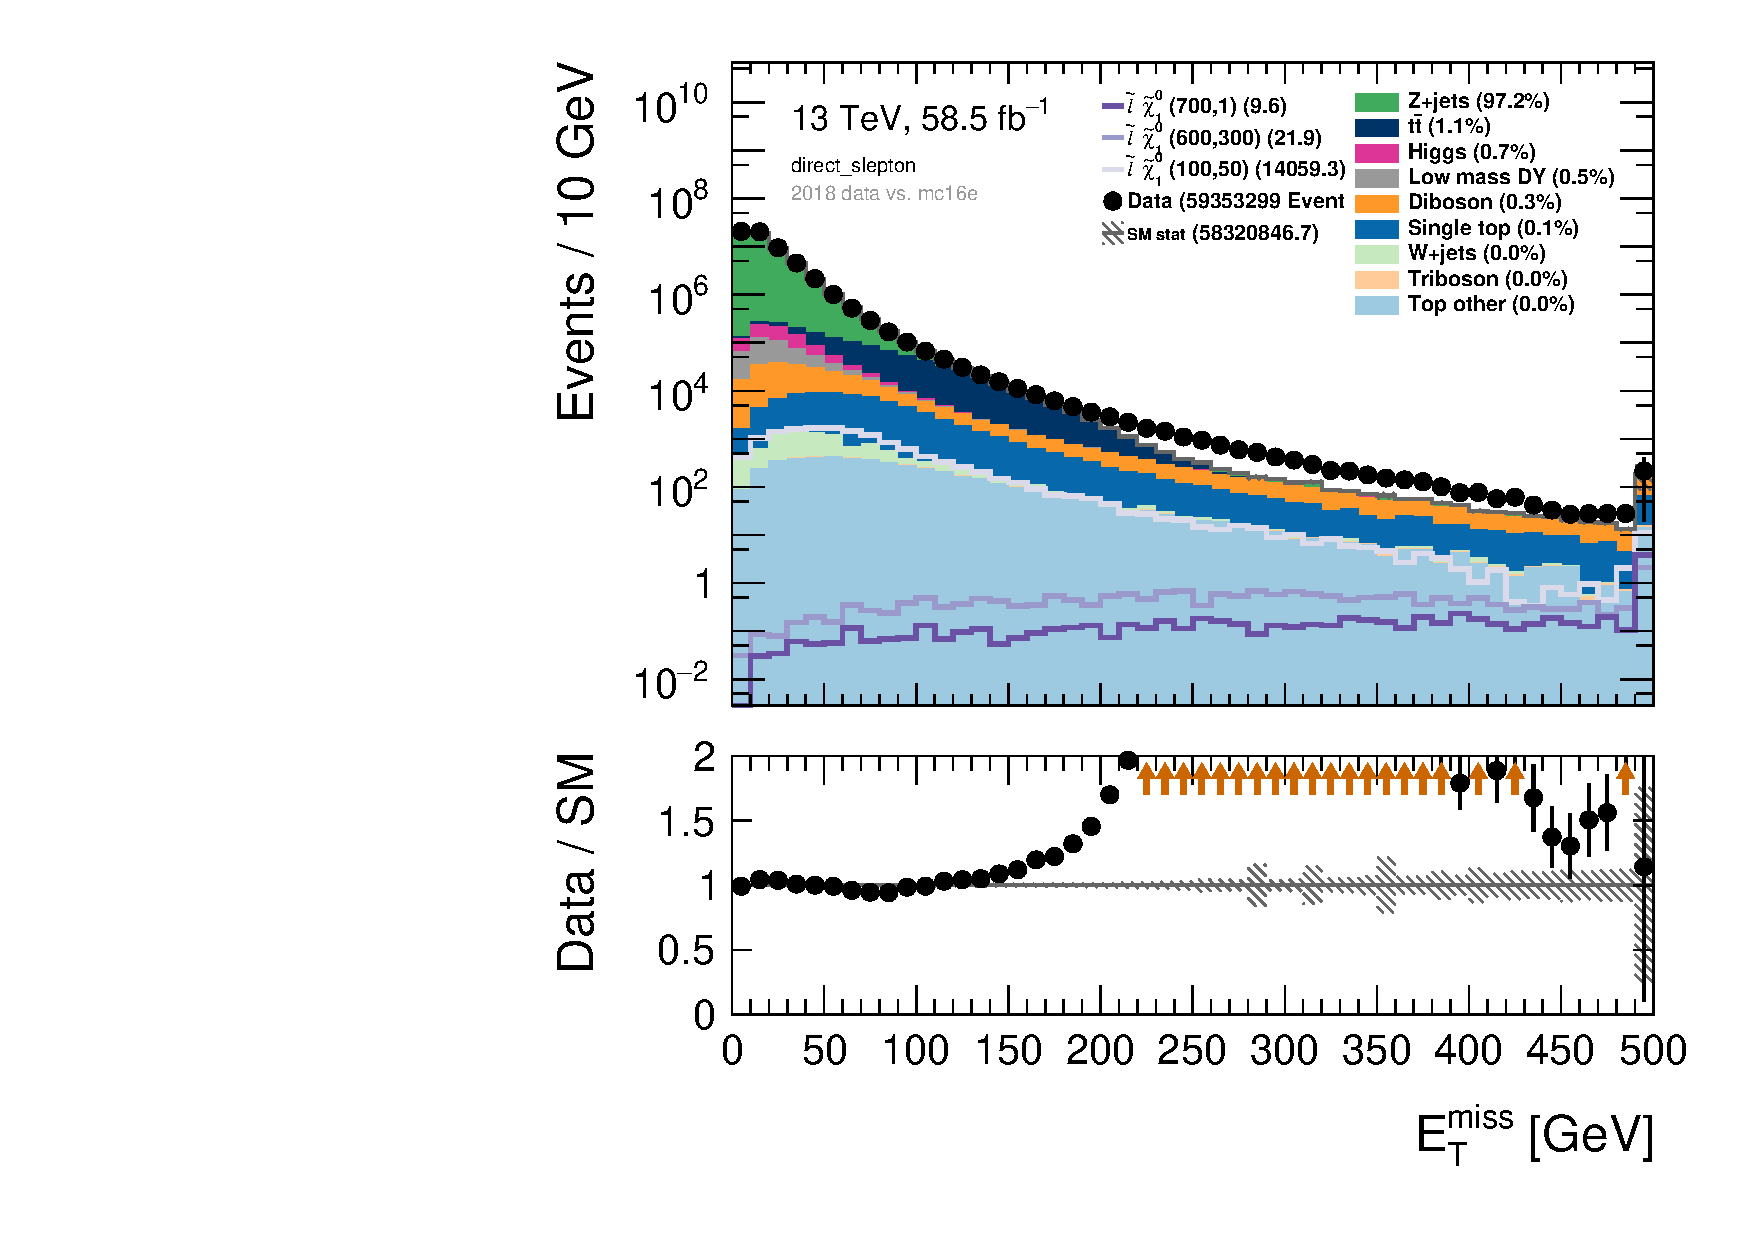
\includegraphics[width=\textwidth]{Figures/SlepSlep/CutAndCount/1stcut_2L+OS/hist1d_met_Et_direct_slepton.pdf}
    \caption{Missing transverse energy}
    \label{fig:my_label}
    \end{subfigure}
    \\
    \begin{subfigure}[t!]{0.49\textwidth}
        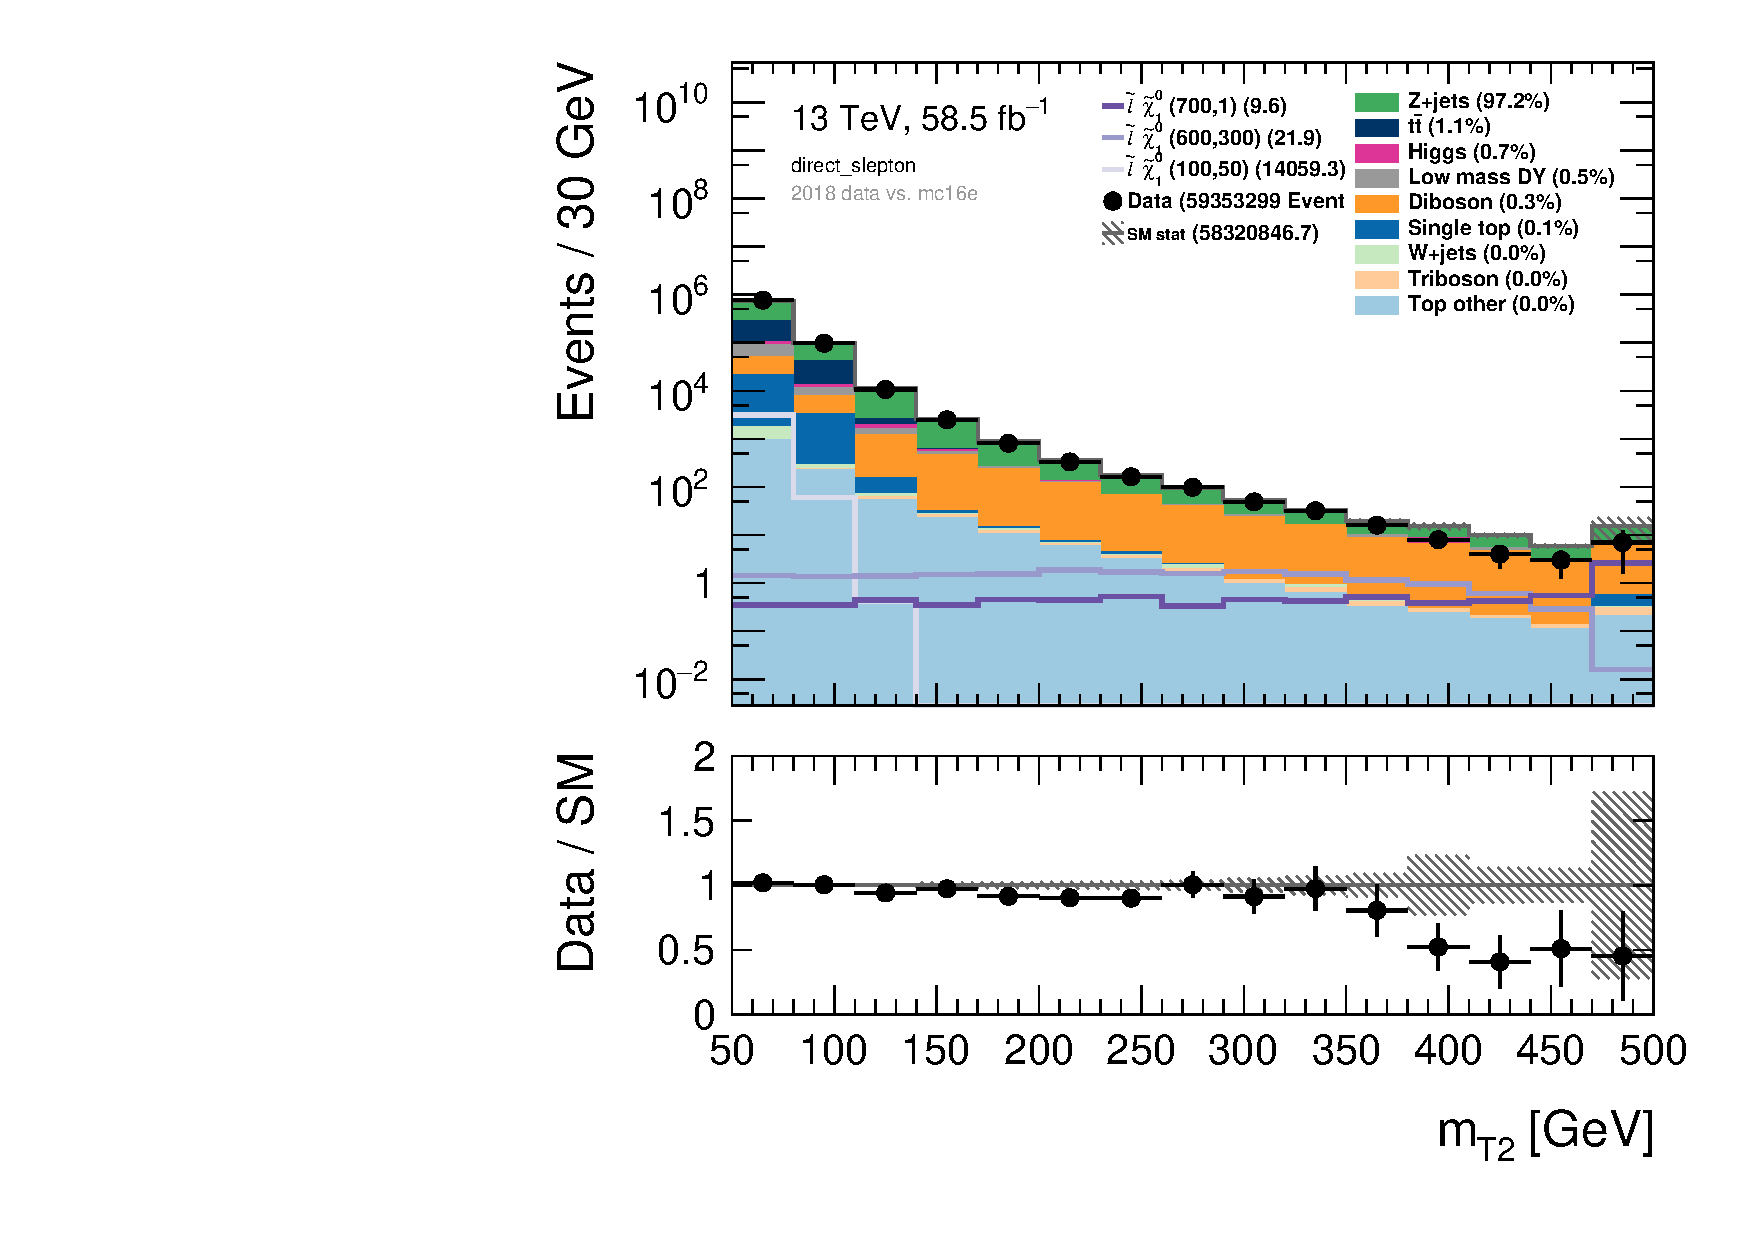
\includegraphics[width=\textwidth]{Figures/SlepSlep/CutAndCount/1stcut_2L+OS/hist1d_mt2_direct_slepton.pdf}
    \caption{Stransverse mass}
    \label{fig:my_label}
    \end{subfigure}
    \begin{subfigure}[t!]{0.49\textwidth}
        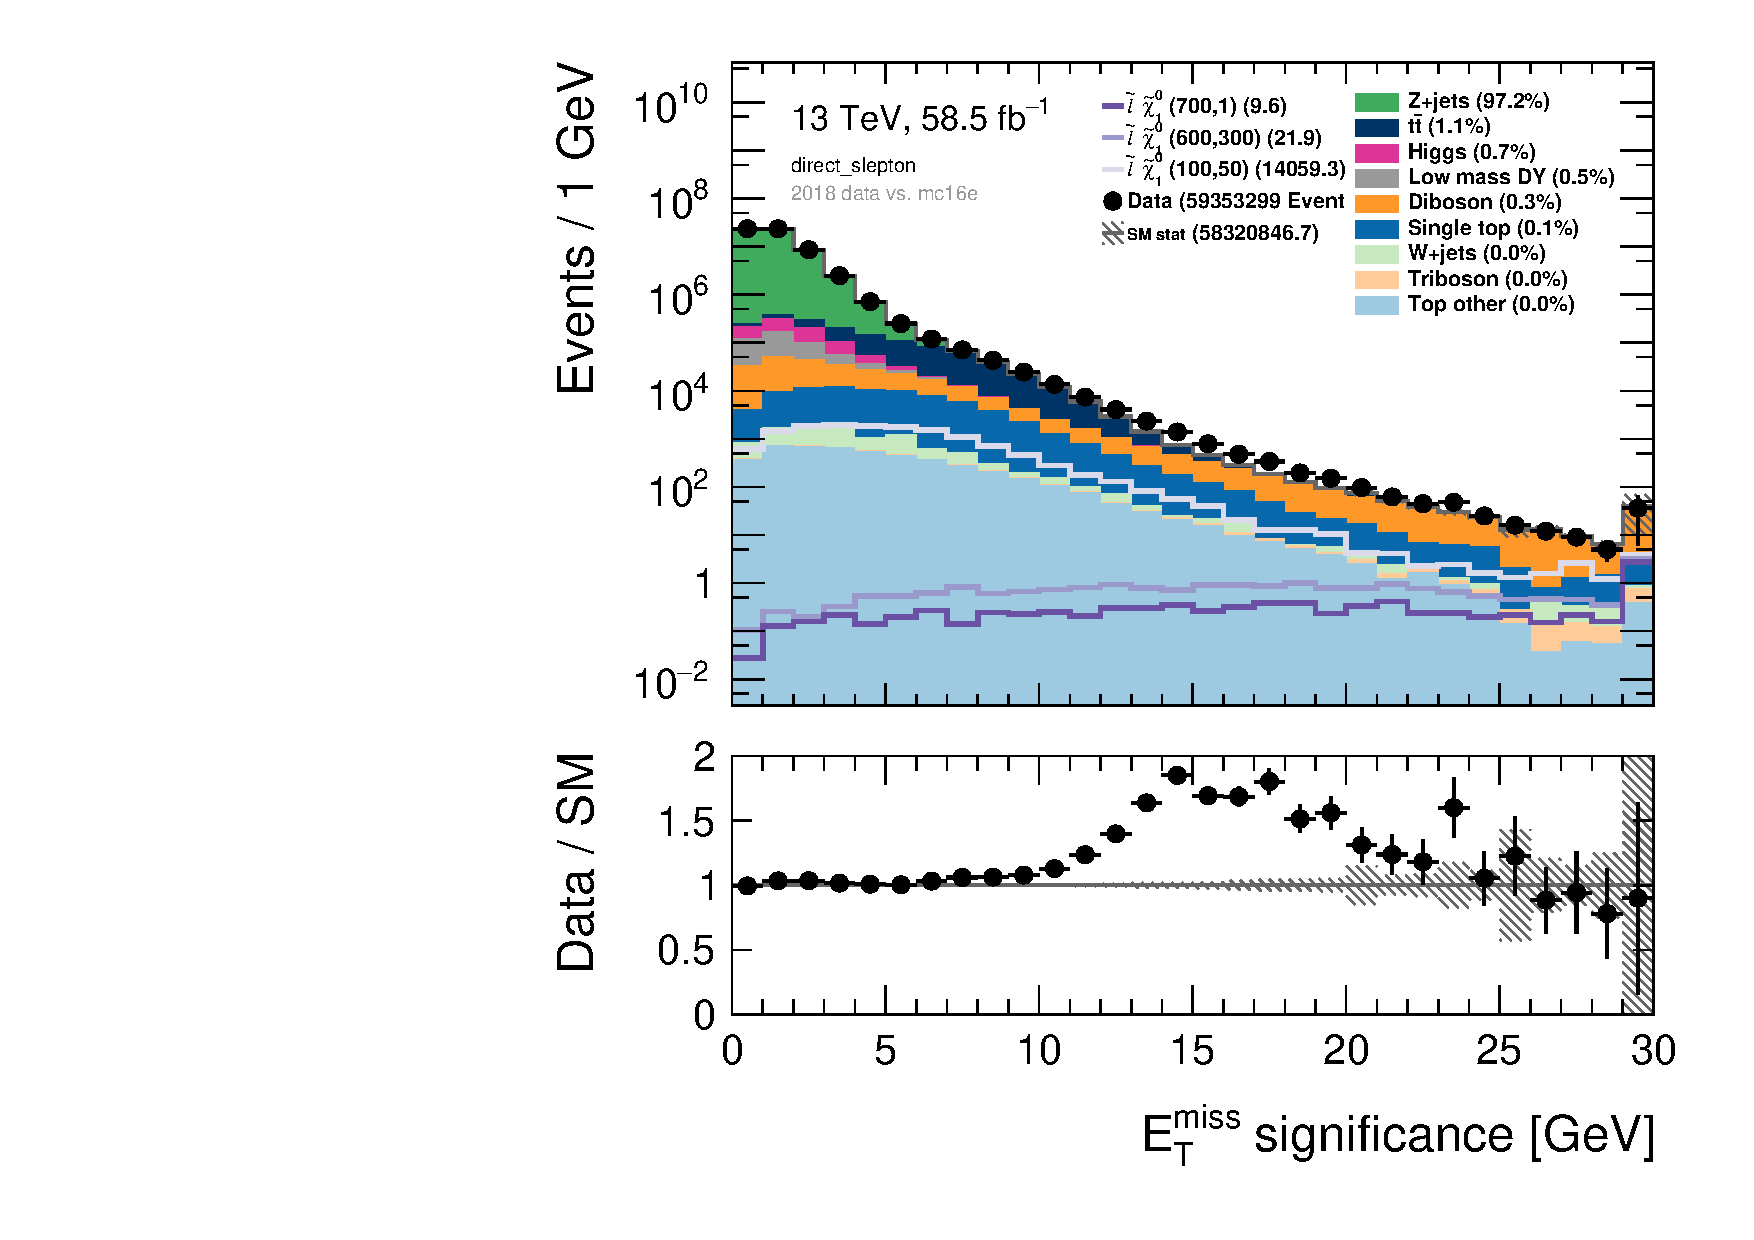
\includegraphics[width=\textwidth]{Figures/SlepSlep/CutAndCount/1stcut_2L+OS/hist1d_met_Sign_direct_slepton.pdf}
    \caption{Missing transverse energy significance}
    \label{fig:my_label}
    \end{subfigure}
    \caption{Plot of the four most important variables in direct slepton production with a cut on only two leptons with opposite charge in the final state.}
    \label{fig:slepslep1stcut}
\end{figure}


After adding a met cut and doing a Z-veto we get the results in figure \ref{fig:slepslep3rdcut} where we can see that Z + jets is reduced a lot. For most of the variables we can now see that the $t\Bar{t}$ is the dominating background, but the signal is still below the backgrounds so we need to add some more cuts.

\begin{figure}[H]
%\begin{minipage}{2\textwidth}
%\begin{adjustwidth}{-3cm}{-3cm}
\centering
%\advance\leftskip-4cm 
%\advance\rightskip-4cm 
    \begin{subfigure}[t!]{0.49\textwidth}
        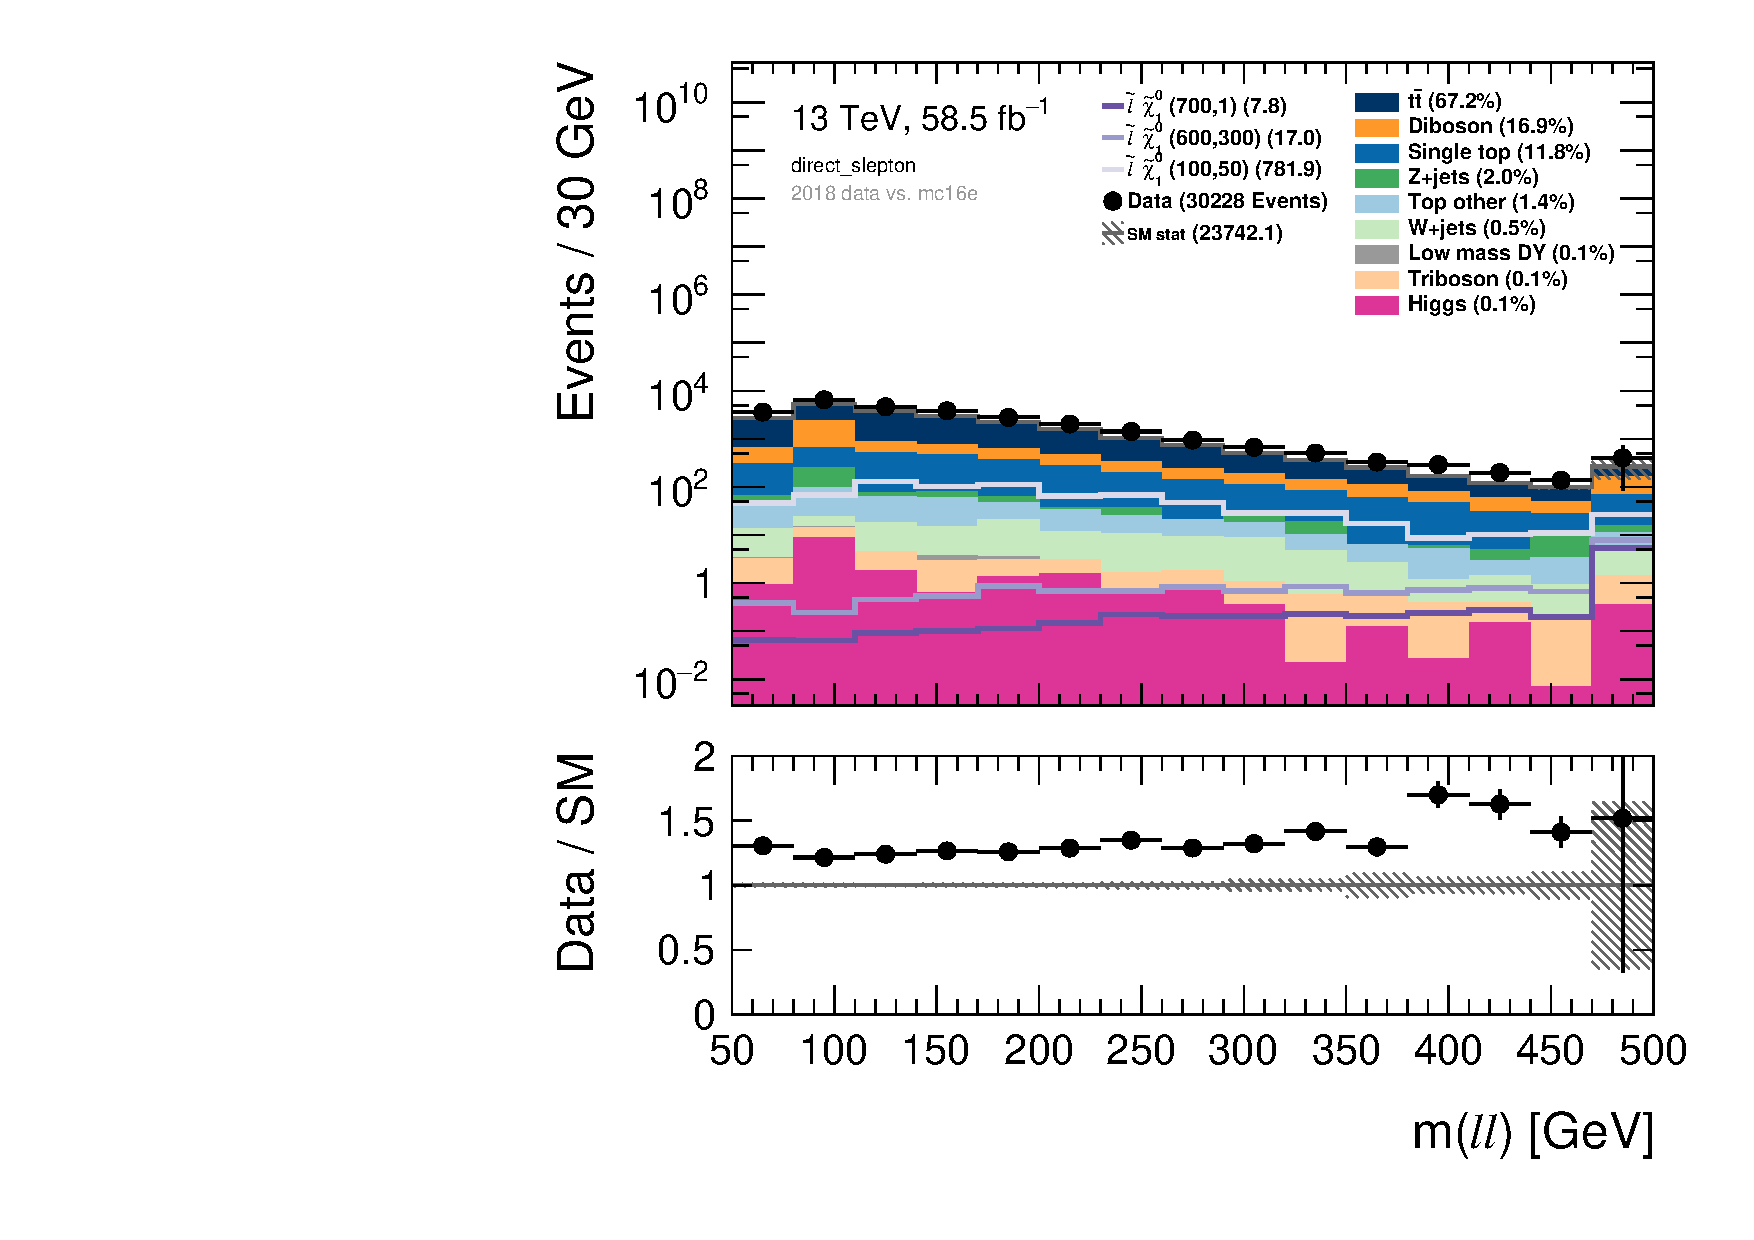
\includegraphics[width=\textwidth]{Figures/SlepSlep/CutAndCount/3rdcut_Zveto/hist1d_mll_direct_slepton.pdf}
    \caption{Invariant mass}
    \label{fig:my_label}
    \end{subfigure}
    \begin{subfigure}[t!]{0.49\textwidth}
        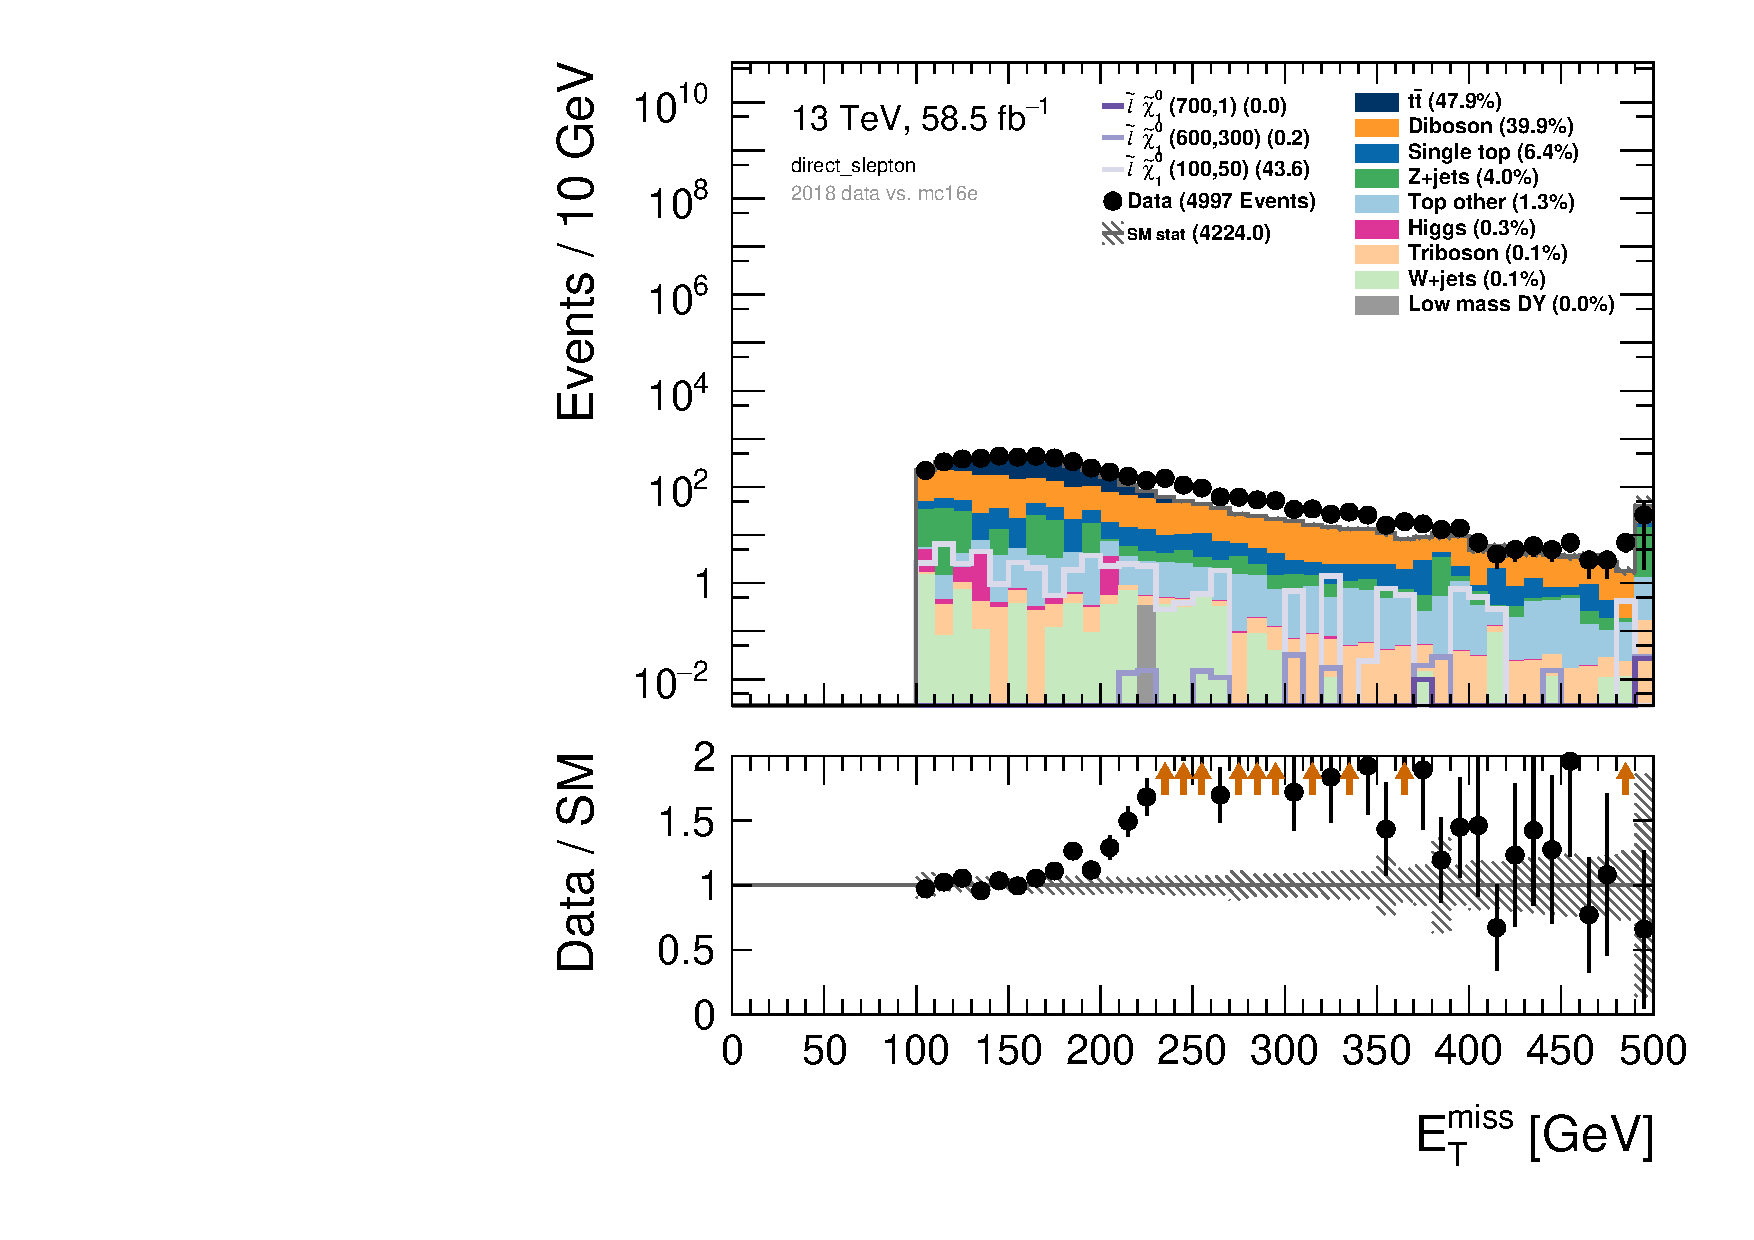
\includegraphics[width=\textwidth]{Figures/SlepSlep/CutAndCount/3rdcut_Zveto/hist1d_met_Et_direct_slepton.pdf}
    \caption{Missing transverse energy}
    \label{fig:my_label}
    \end{subfigure}
    \\
    \begin{subfigure}[t!]{0.49\textwidth}
        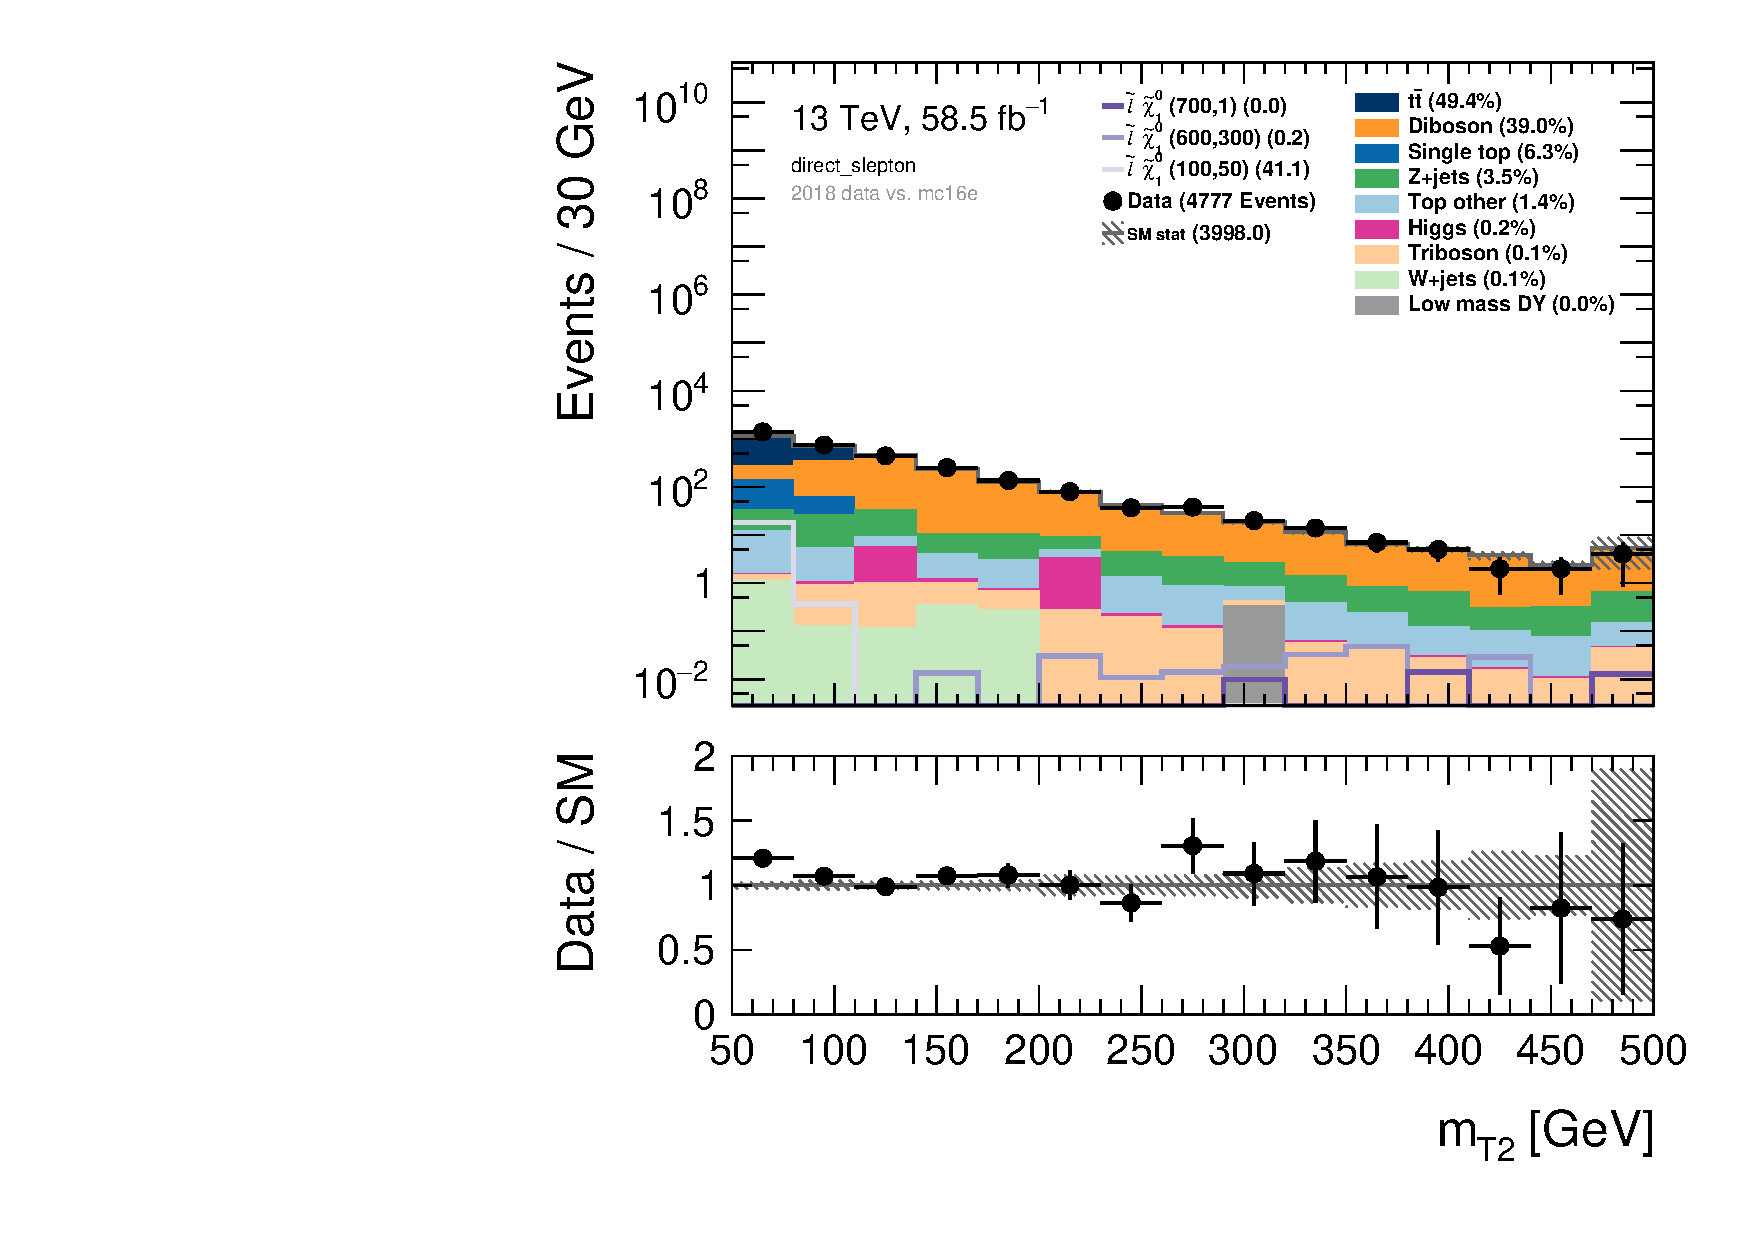
\includegraphics[width=\textwidth]{Figures/SlepSlep/CutAndCount/3rdcut_Zveto/hist1d_mt2_direct_slepton.pdf}
    \caption{Stransverse mass}
    \label{fig:my_label}
    \end{subfigure}
    \begin{subfigure}[t!]{0.49\textwidth}
        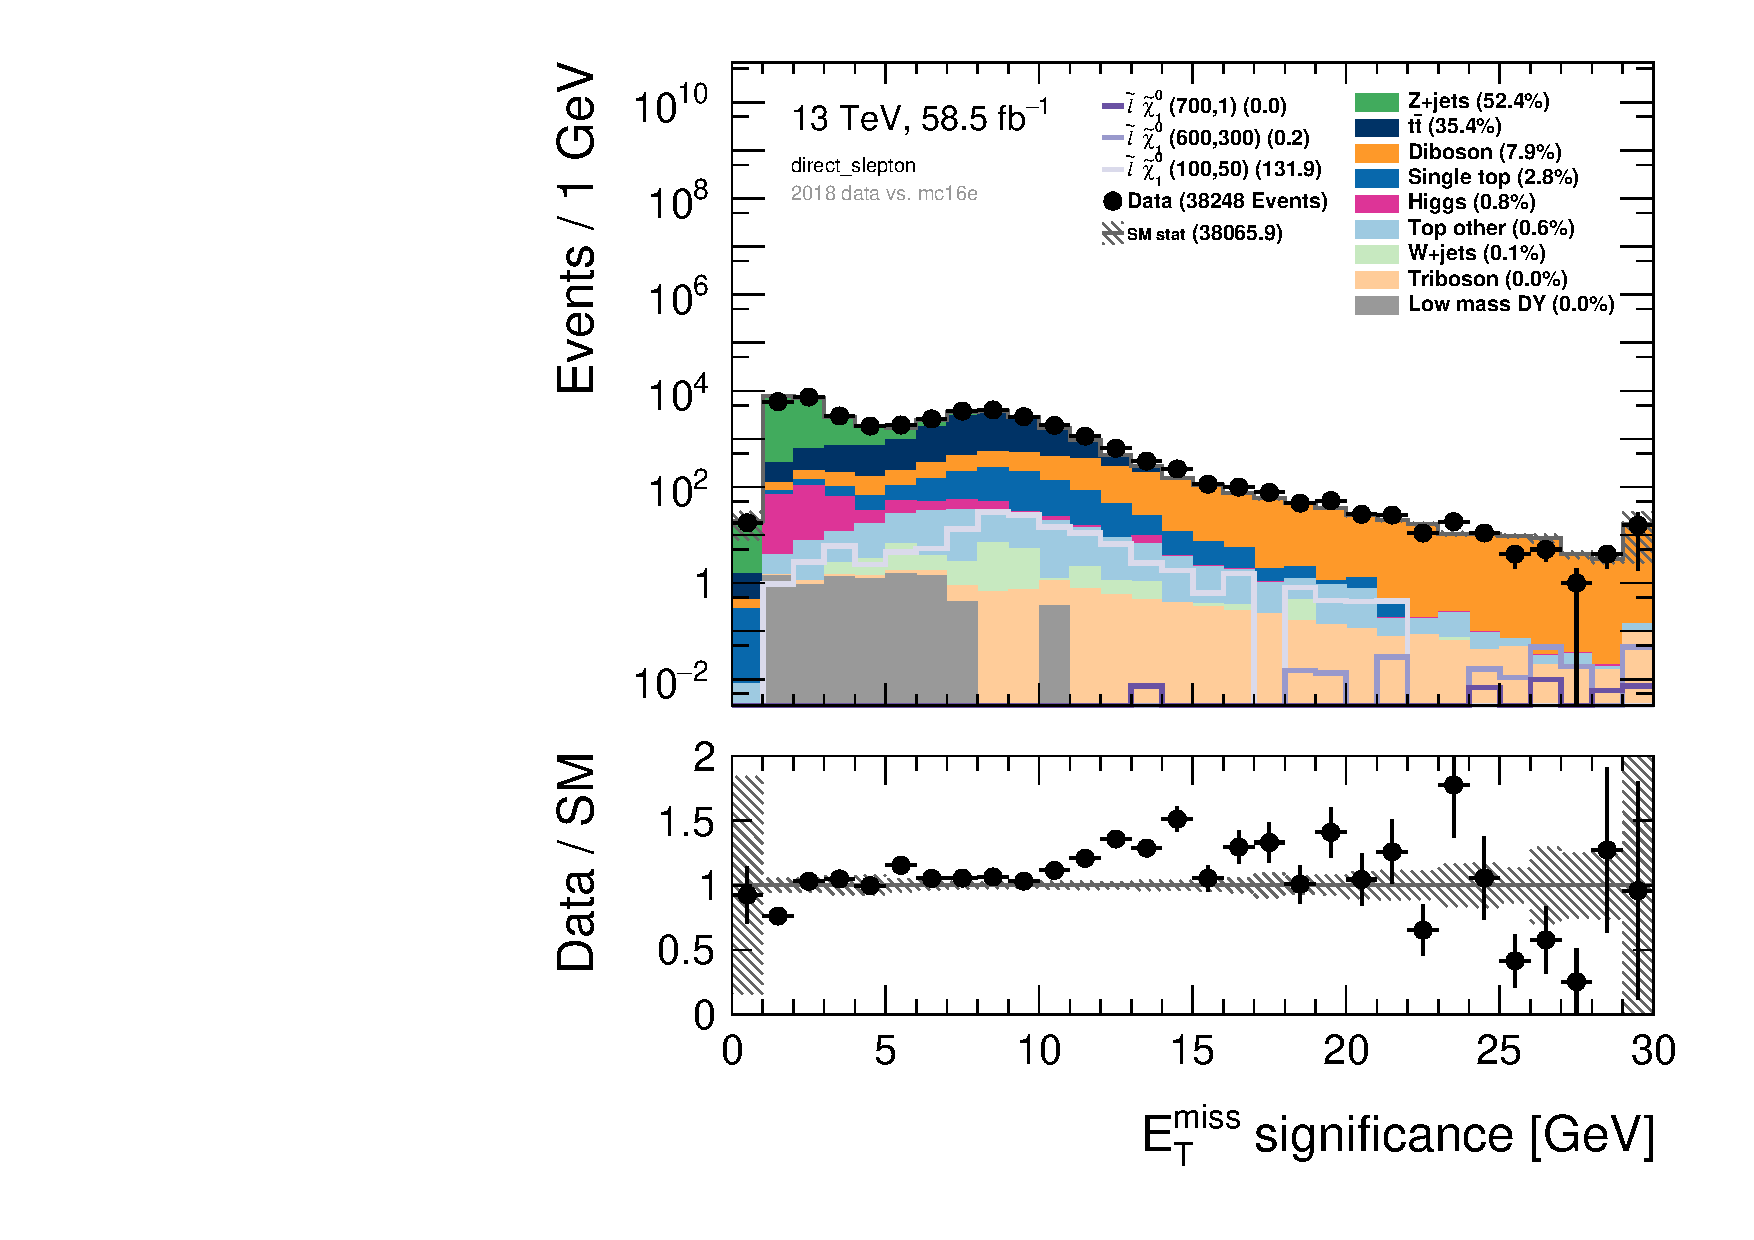
\includegraphics[width=\textwidth]{Figures/SlepSlep/CutAndCount/3rdcut_Zveto/hist1d_met_Sign_direct_slepton.pdf}
    \caption{Missing transverse energy significance}
    \label{fig:my_label}
    \end{subfigure}
    \caption{Plot of the four most important variables in direct slepton production with a cut on $E_T^{miss} >110$, $E_T^{miss}$ significance $>10$ and a Z-veto in addition to the previous cuts.}
    \label{fig:slepslep3rdcut}
\end{figure}



After adding some jet cuts (number of jets with $p_T$> 30GeV = 0 and a b-jet veto) we get the results in figure \ref{fig:slepslep4th_3_cut}. We can see that we succeeded on reducing the $t\Bar{t}$ background as well and we now have diboson as the dominating background.

\begin{figure}[H]
%\begin{minipage}{2\textwidth}
%\begin{adjustwidth}{-3cm}{-3cm}
\centering
%\advance\leftskip-4cm 
%\advance\rightskip-4cm 
    \begin{subfigure}[t!]{0.49\textwidth}
        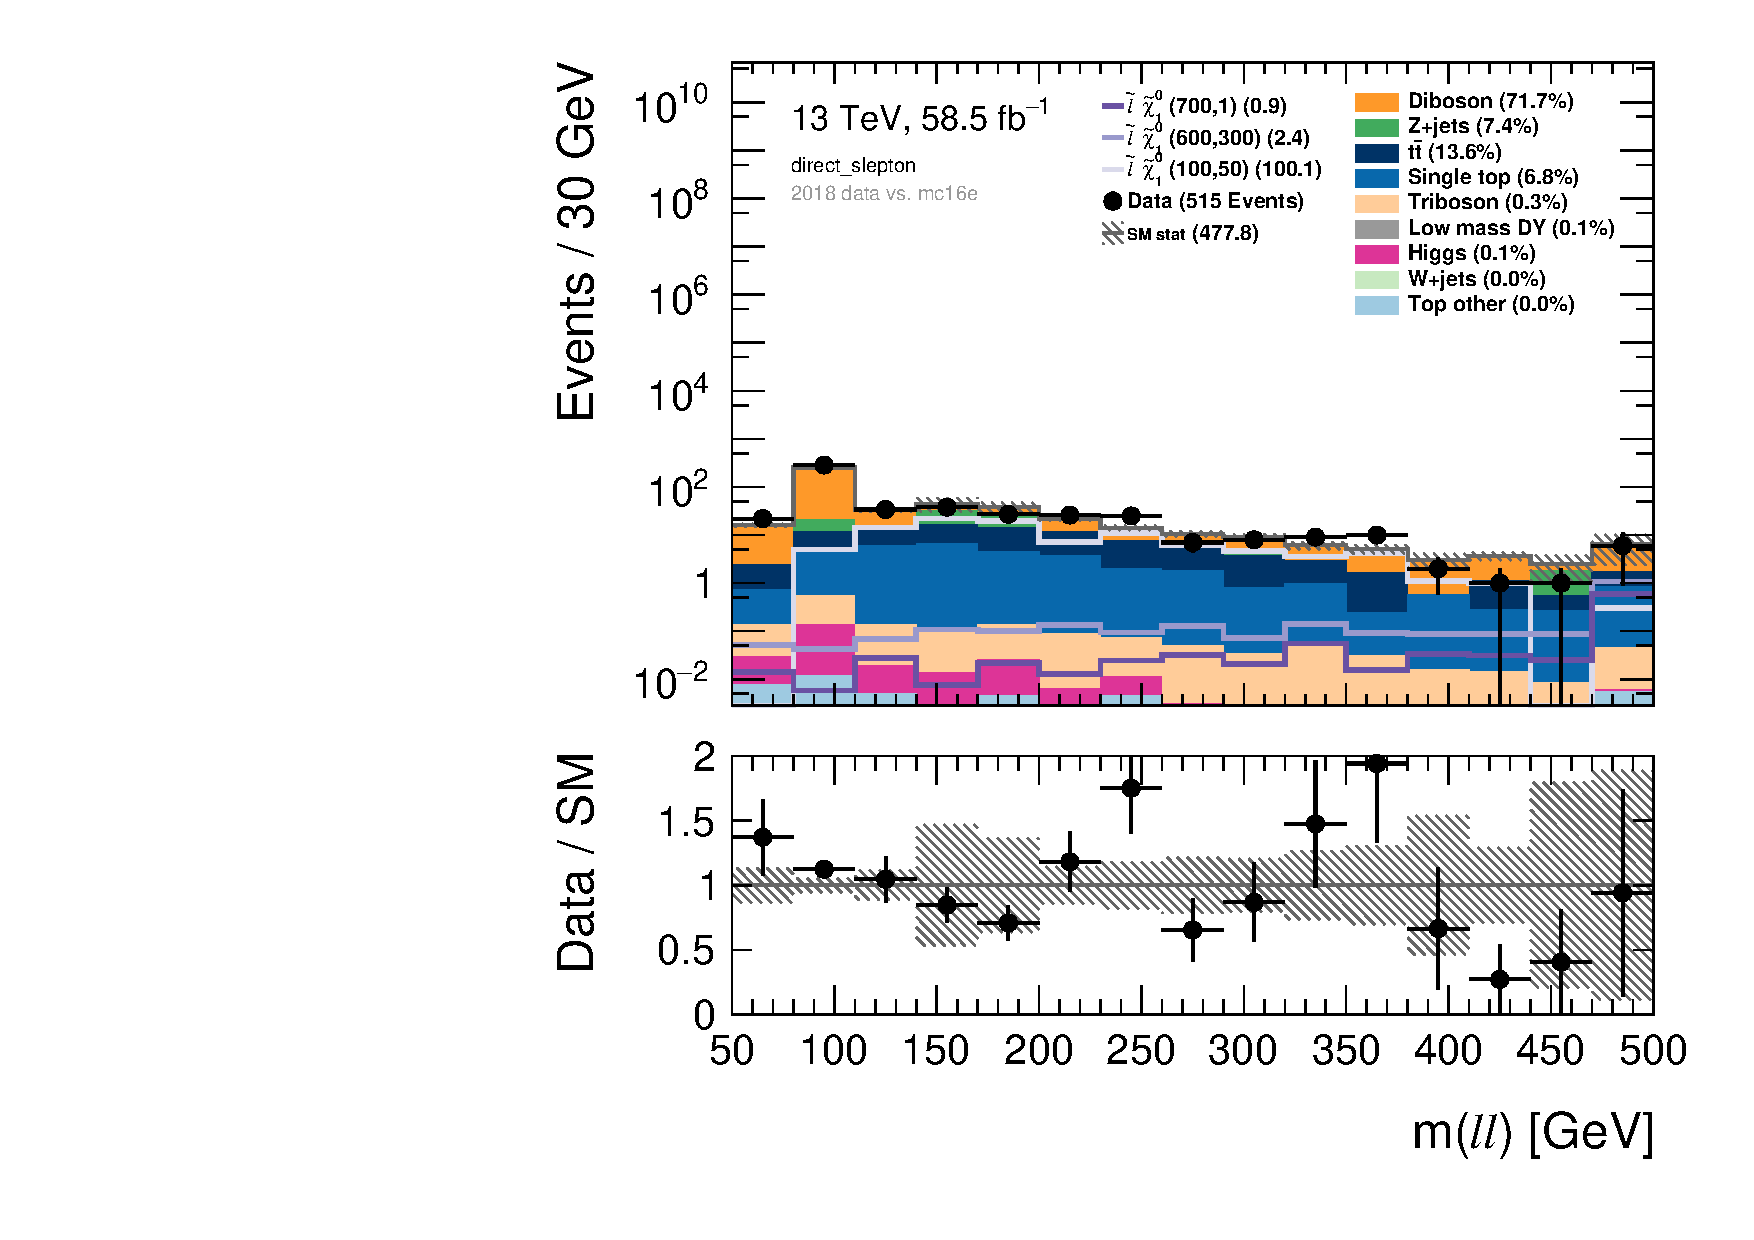
\includegraphics[width=\textwidth]{Figures/SlepSlep/CutAndCount/4thcut_3_Bjets/hist1d_mll_direct_slepton.pdf}
    \caption{Invariant mass}
    \label{fig:my_label}
    \end{subfigure}
    \begin{subfigure}[t!]{0.49\textwidth}
        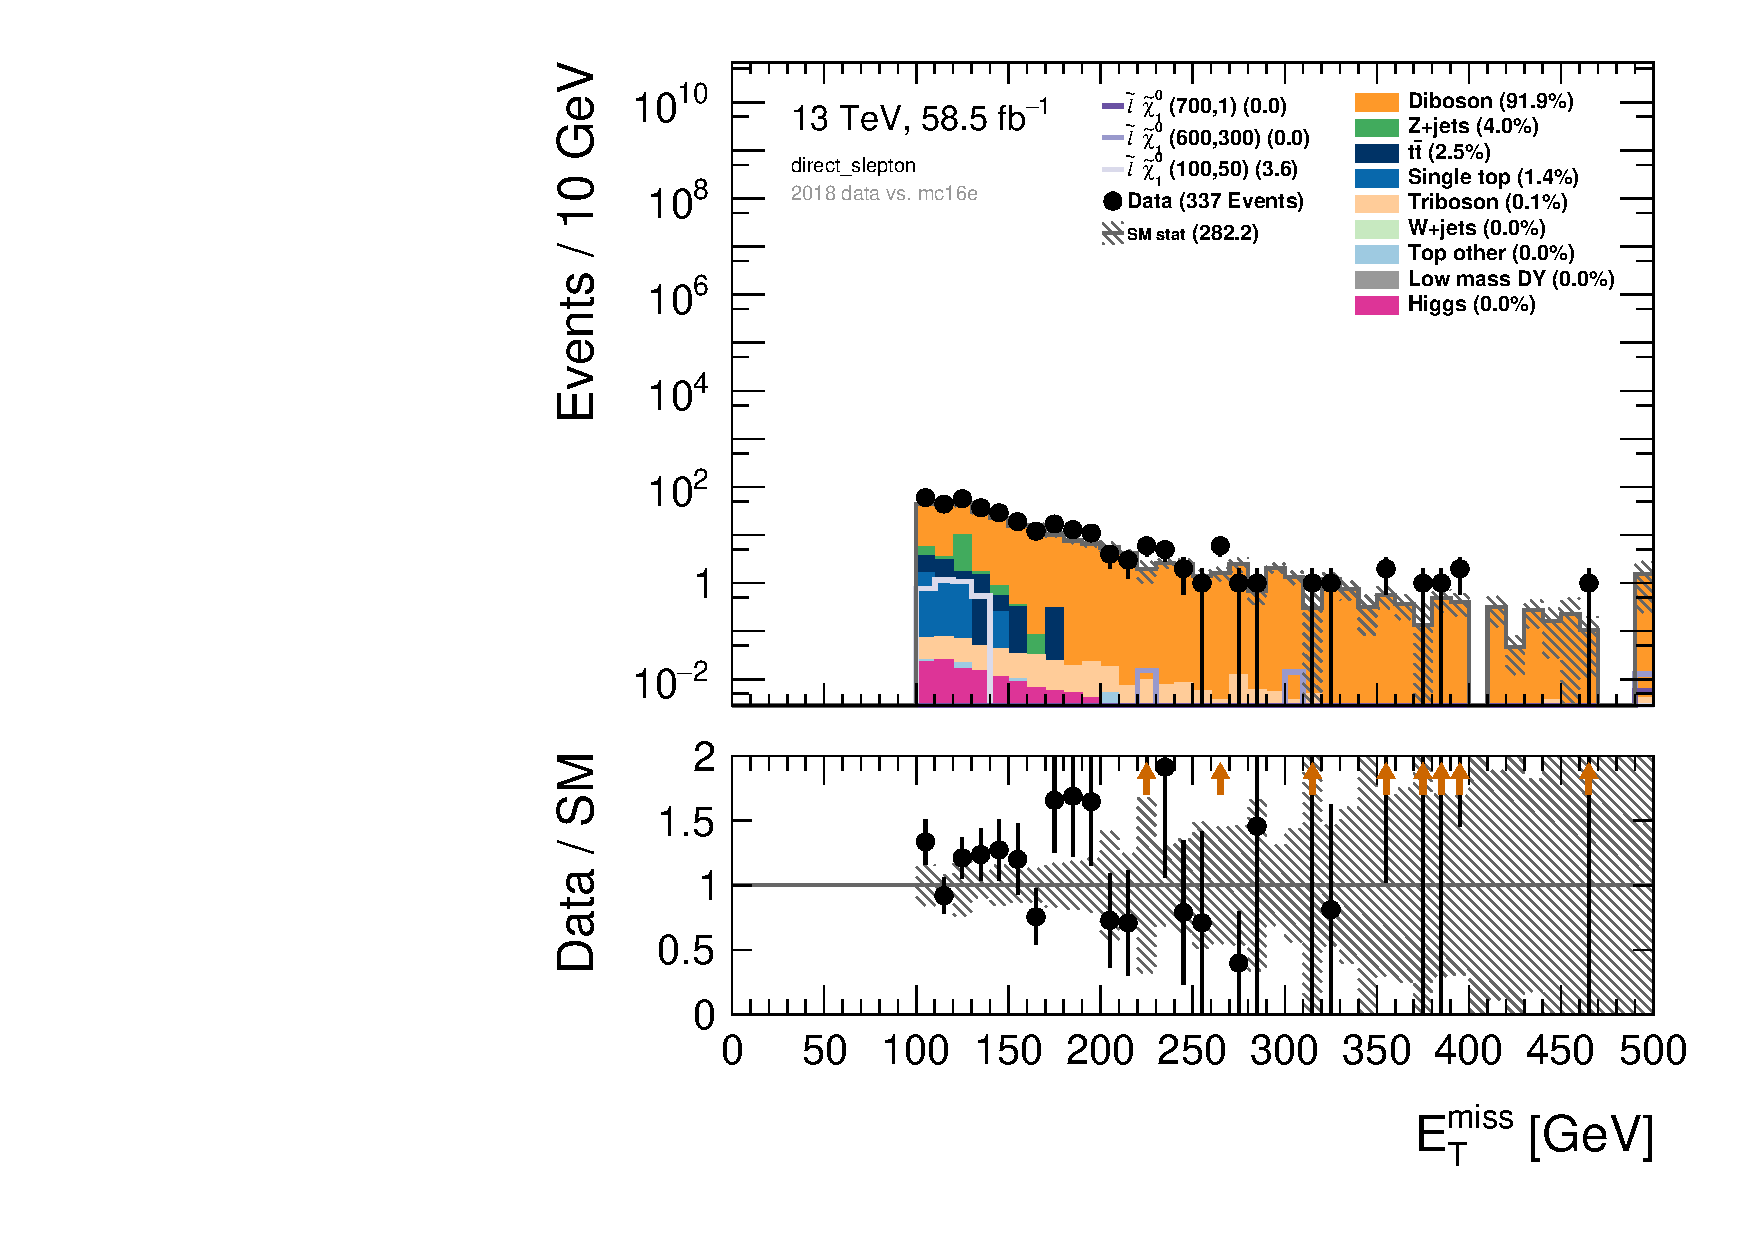
\includegraphics[width=\textwidth]{Figures/SlepSlep/CutAndCount/4thcut_3_Bjets/hist1d_met_Et_direct_slepton.pdf}
    \caption{Missing transverse energy}
    \label{fig:my_label}
    \end{subfigure}
    \\
    \begin{subfigure}[t!]{0.49\textwidth}
        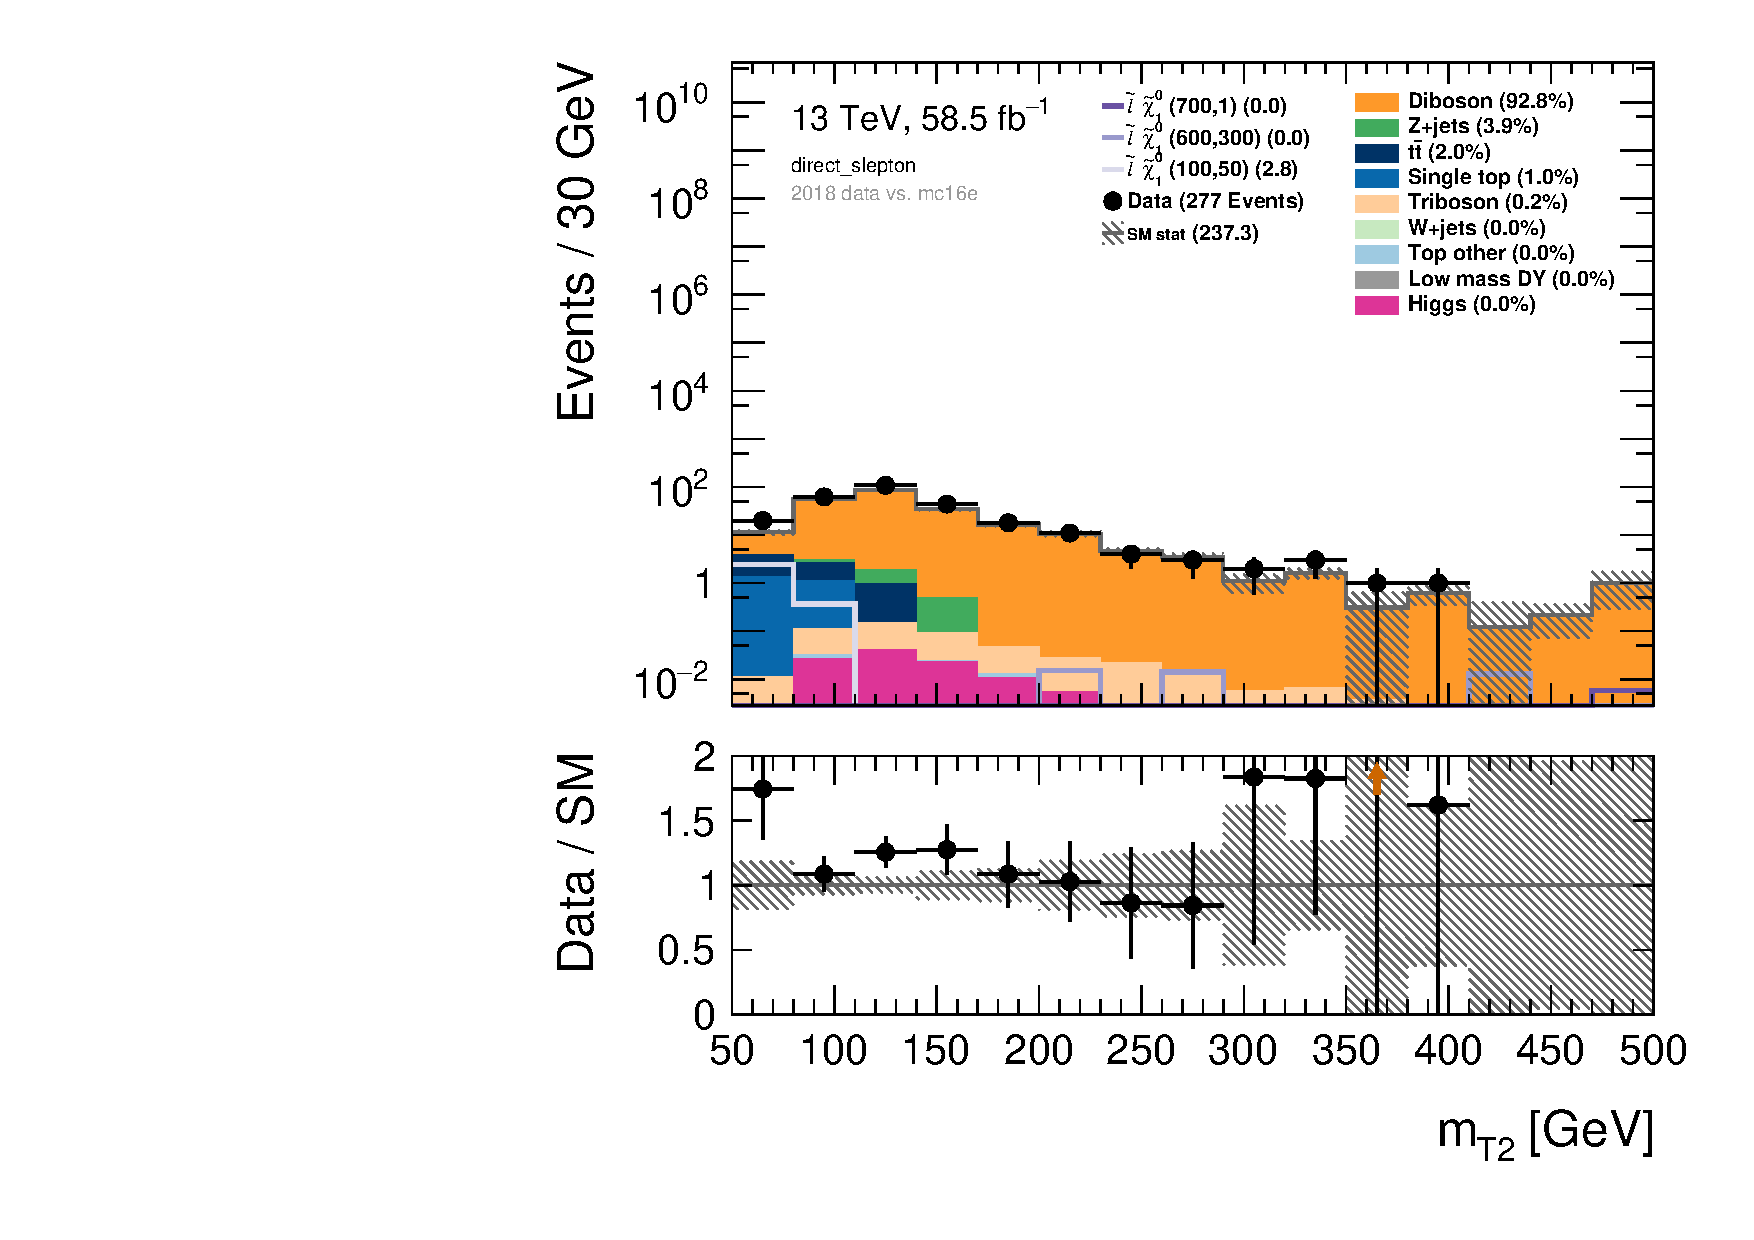
\includegraphics[width=\textwidth]{Figures/SlepSlep/CutAndCount/4thcut_3_Bjets/hist1d_mt2_direct_slepton.pdf}
    \caption{Stransverse mass}
    \label{fig:my_label}
    \end{subfigure}
    \begin{subfigure}[t!]{0.49\textwidth}
        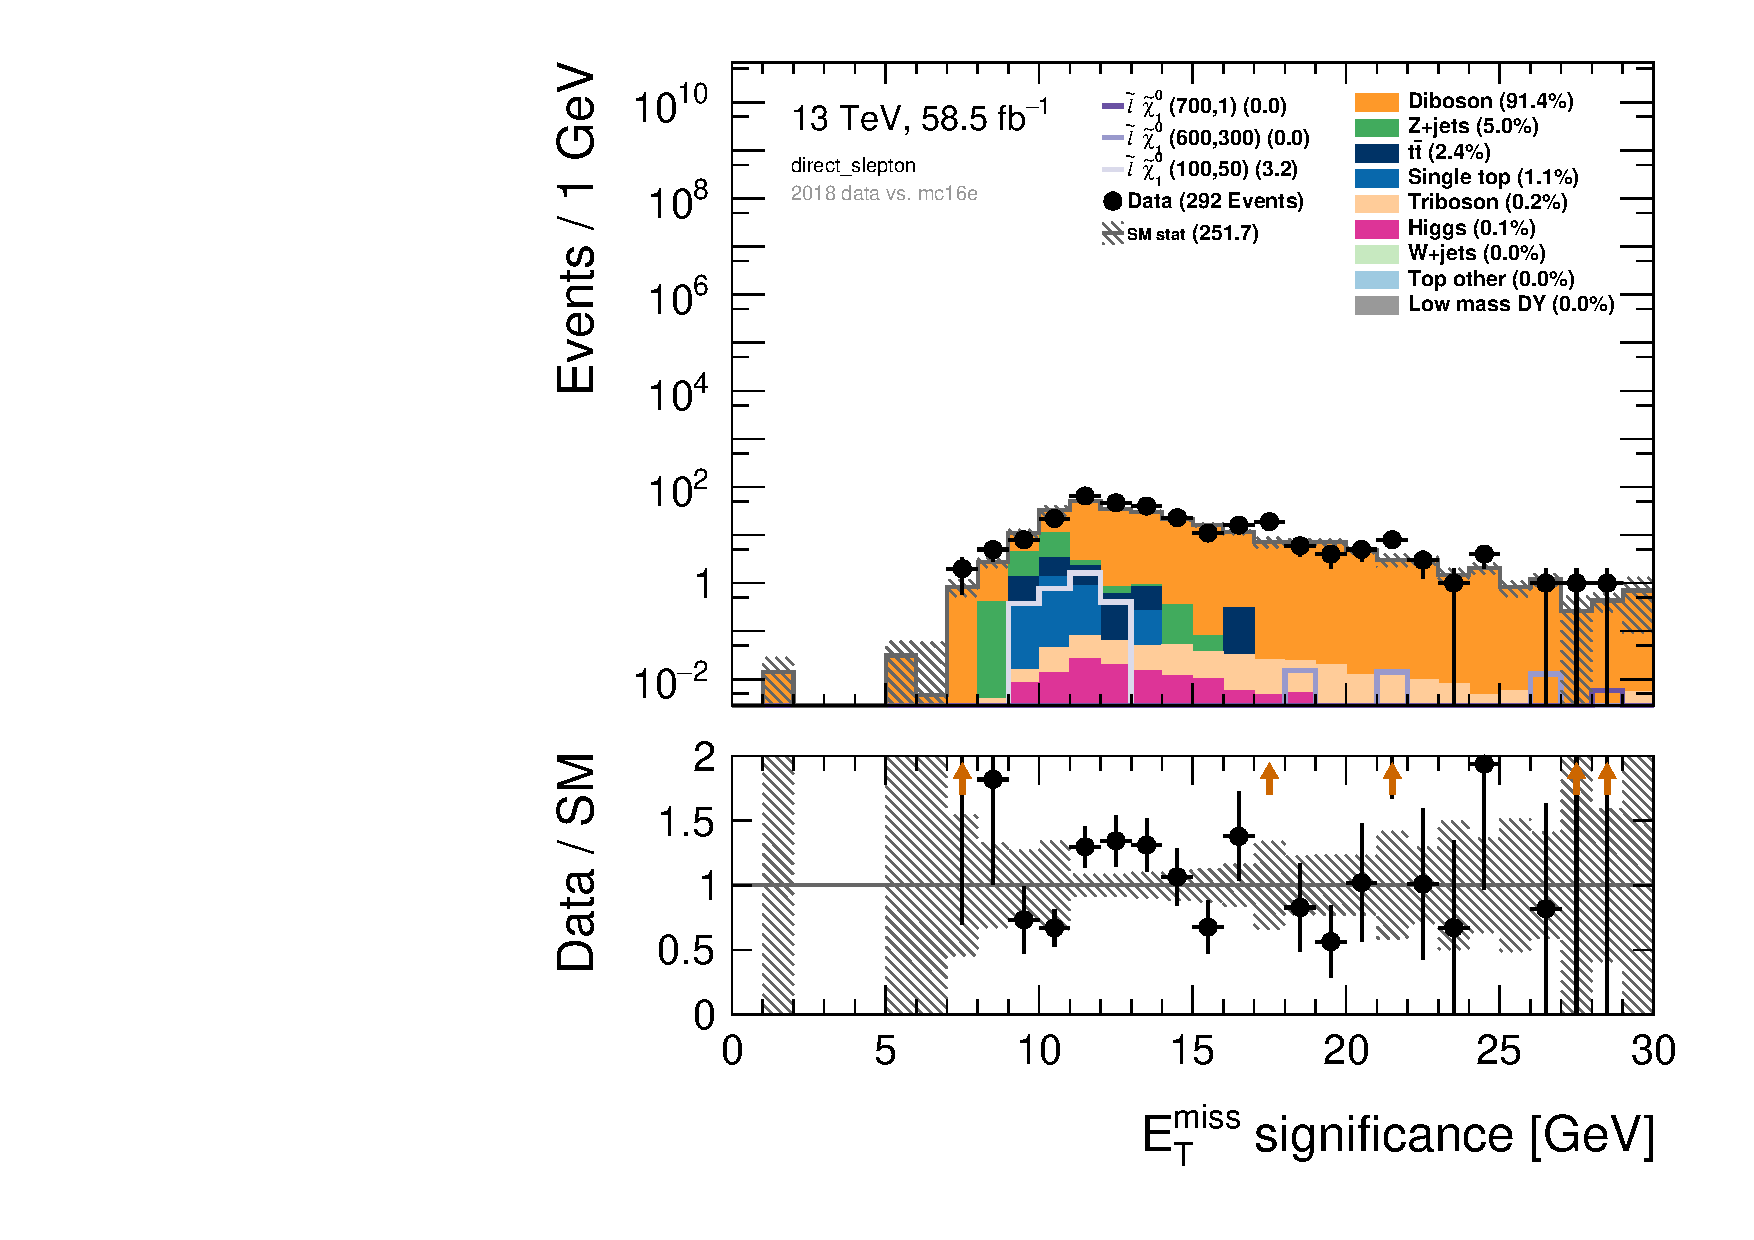
\includegraphics[width=\textwidth]{Figures/SlepSlep/CutAndCount/4thcut_3_Bjets/hist1d_met_Sign_direct_slepton.pdf}
    \caption{Missing transverse energy significance}
    \label{fig:my_label}
    \end{subfigure}
    \caption{Plot of the four most important variables in direct slepton production with a cut on number of jets and b-jets = 0 in addition to the previous cuts.}
    \label{fig:slepslep4th_3_cut}
\end{figure}

After adding one last cut in the $m_{T_2}$  variable we can see that the background doesn't change that much and that our signals is almost cut away as well. 

\begin{figure}[H]
%\begin{minipage}{2\textwidth}
%\begin{adjustwidth}{-3cm}{-3cm}
\centering
%\advance\leftskip-4cm 
%\advance\rightskip-4cm 
    \begin{subfigure}[t!]{0.49\textwidth}
        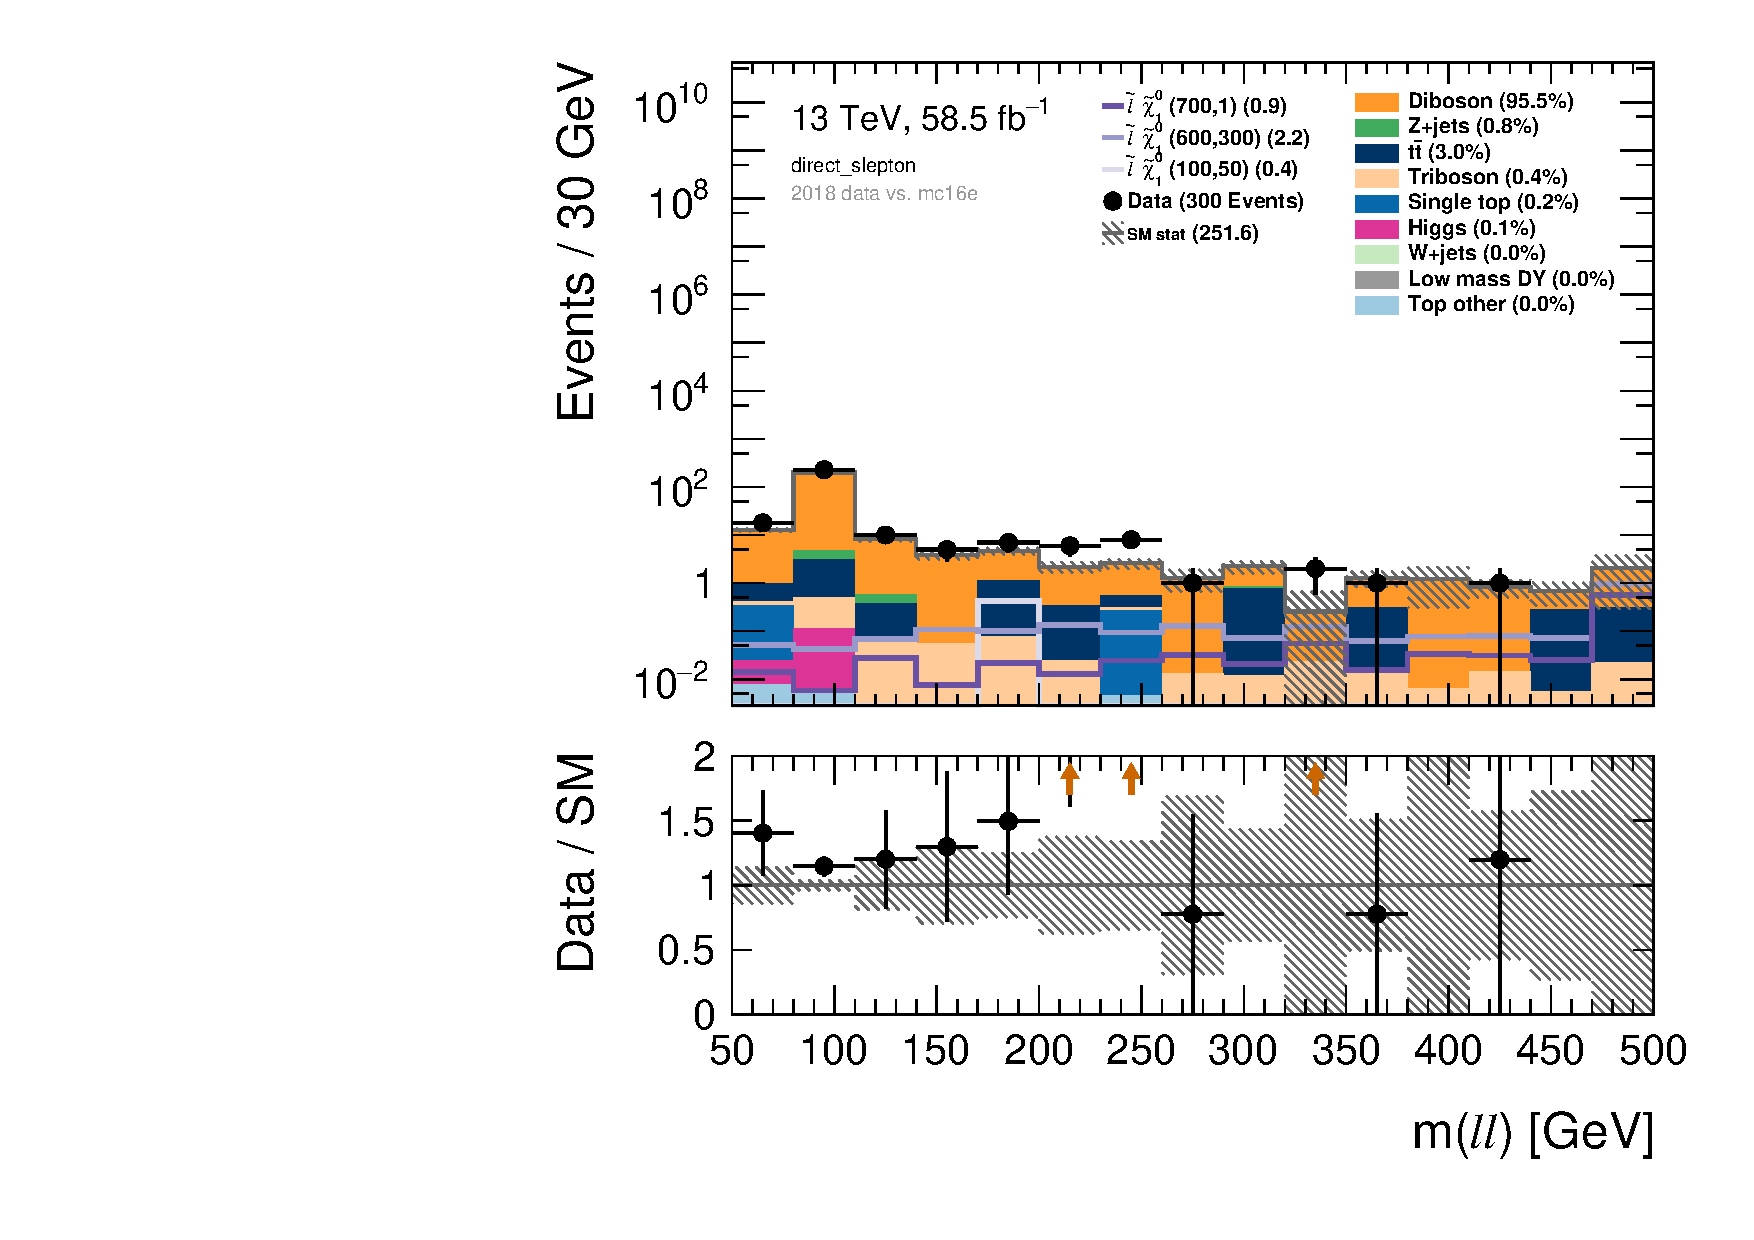
\includegraphics[width=\textwidth]{Figures/SlepSlep/CutAndCount/5thcut_1_mt2_100/hist1d_mll_direct_slepton.pdf}
    \caption{Invariant mass}
    \label{fig:my_label}
    \end{subfigure}
    \begin{subfigure}[t!]{0.49\textwidth}
        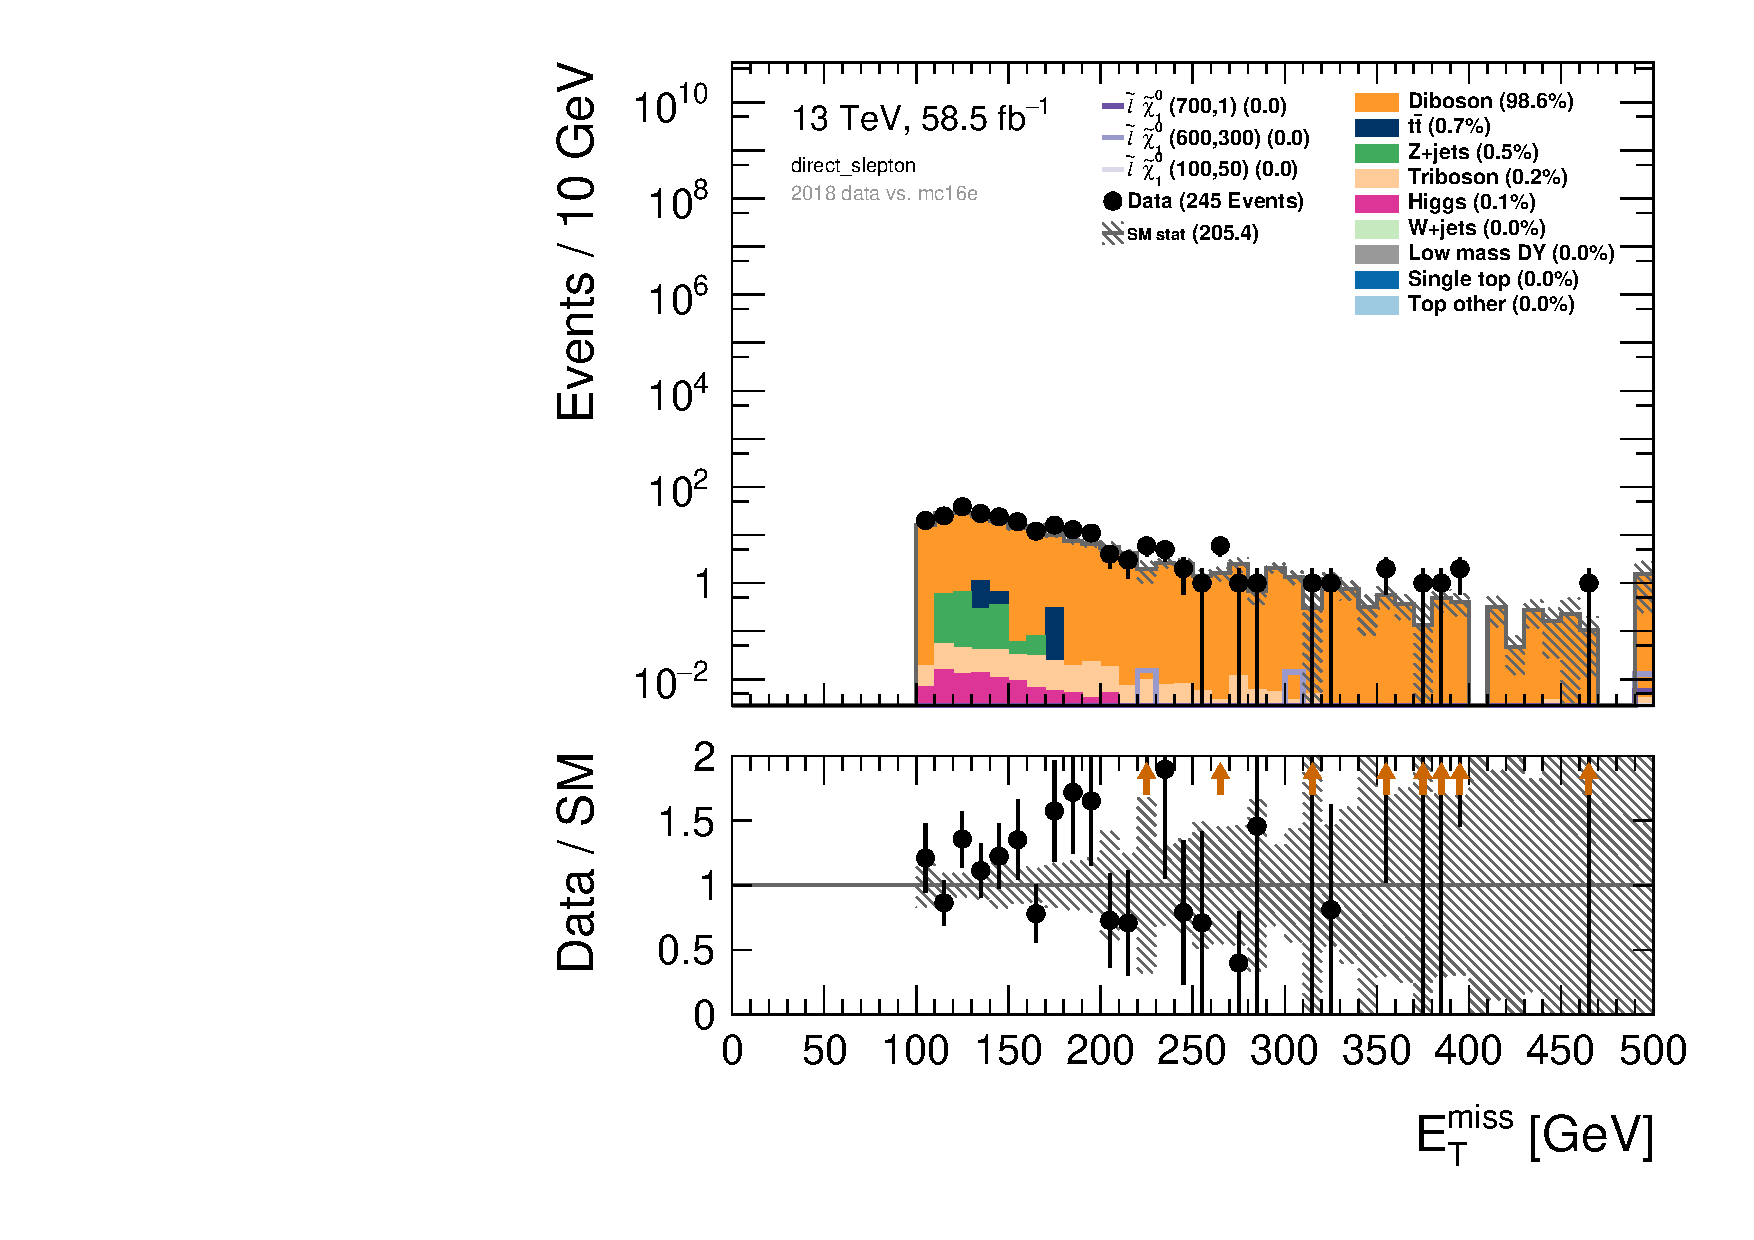
\includegraphics[width=\textwidth]{Figures/SlepSlep/CutAndCount/5thcut_1_mt2_100/hist1d_met_Et_direct_slepton.pdf}
    \caption{Missing transverse energy}
    \label{fig:my_label}
    \end{subfigure}
    \\
    \begin{subfigure}[t!]{0.49\textwidth}
        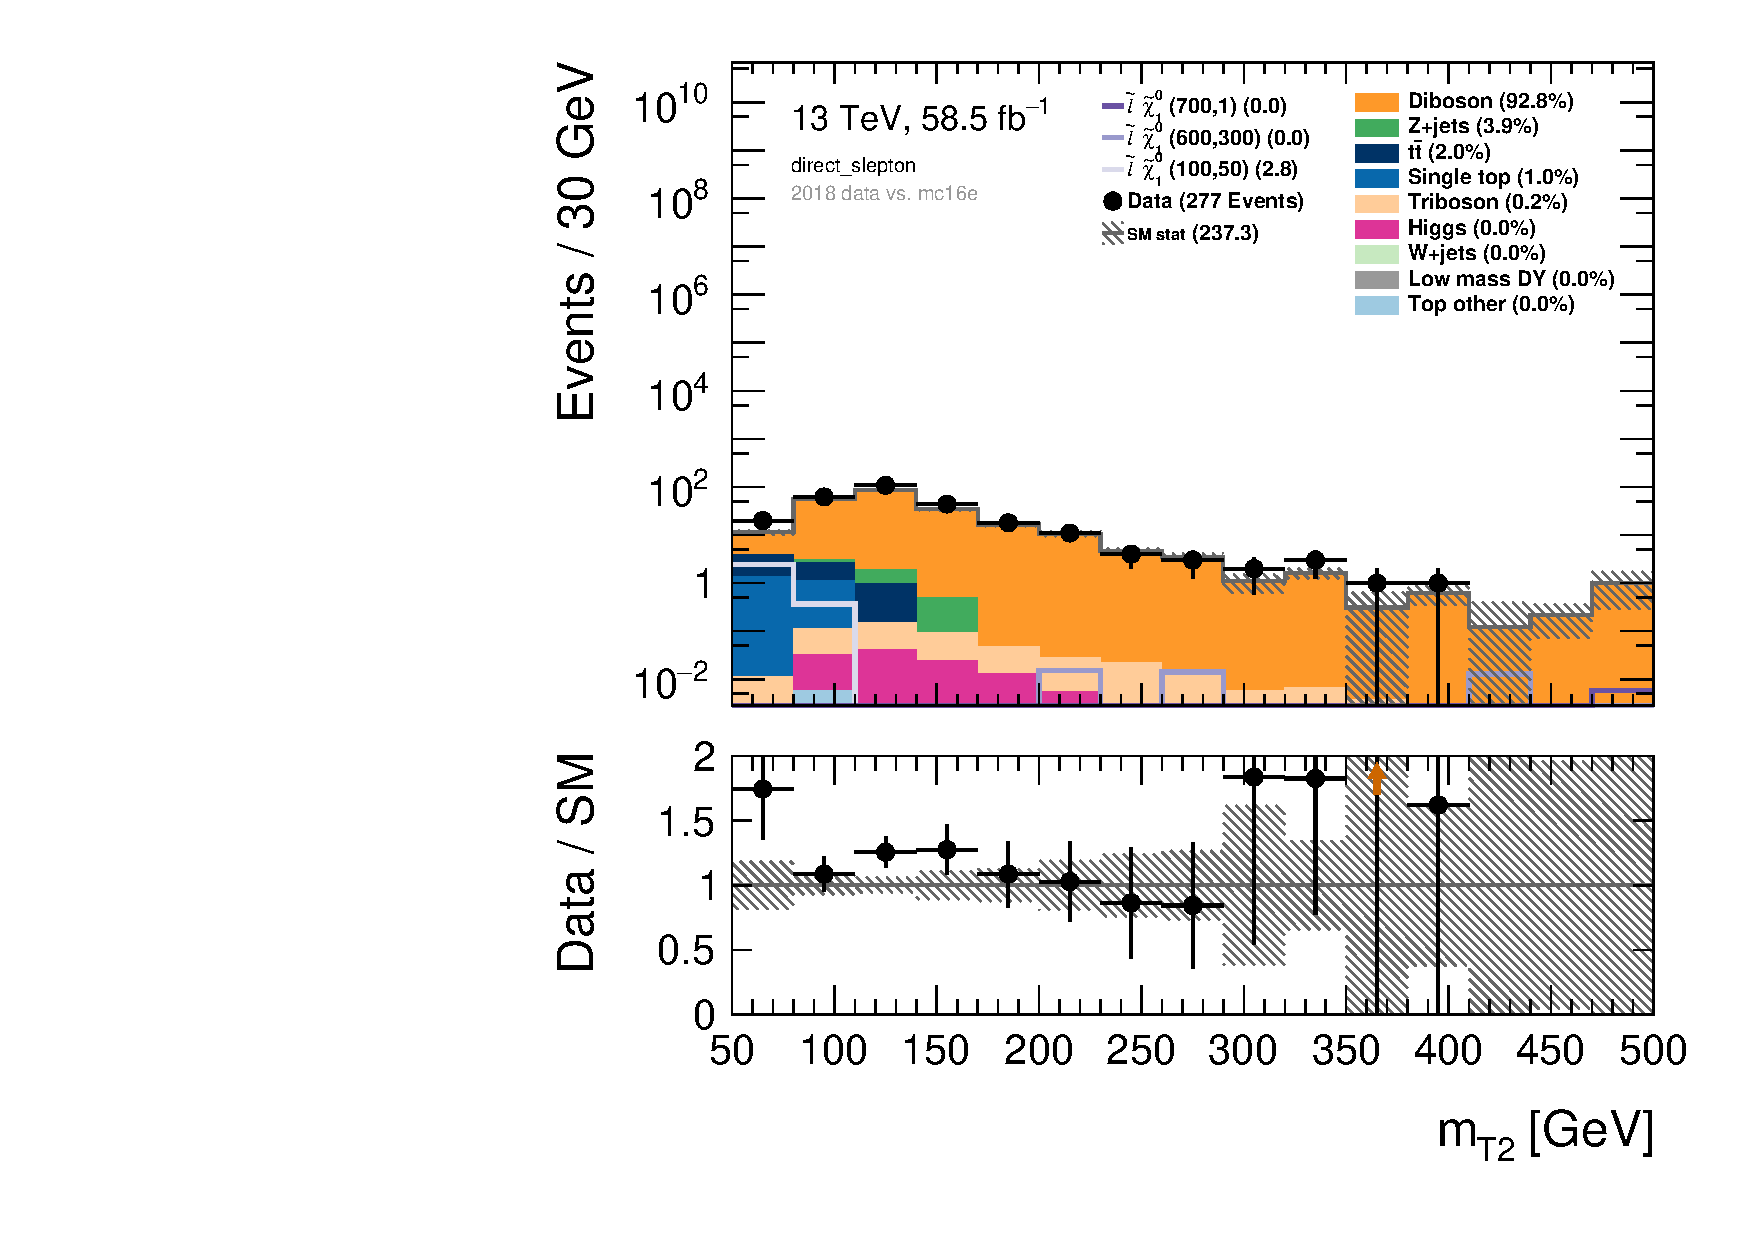
\includegraphics[width=\textwidth]{Figures/SlepSlep/CutAndCount/5thcut_1_mt2_100/hist1d_mt2_direct_slepton.pdf}
    \caption{Stransverse mass}
    \label{fig:my_label}
    \end{subfigure}
    \begin{subfigure}[t!]{0.49\textwidth}
        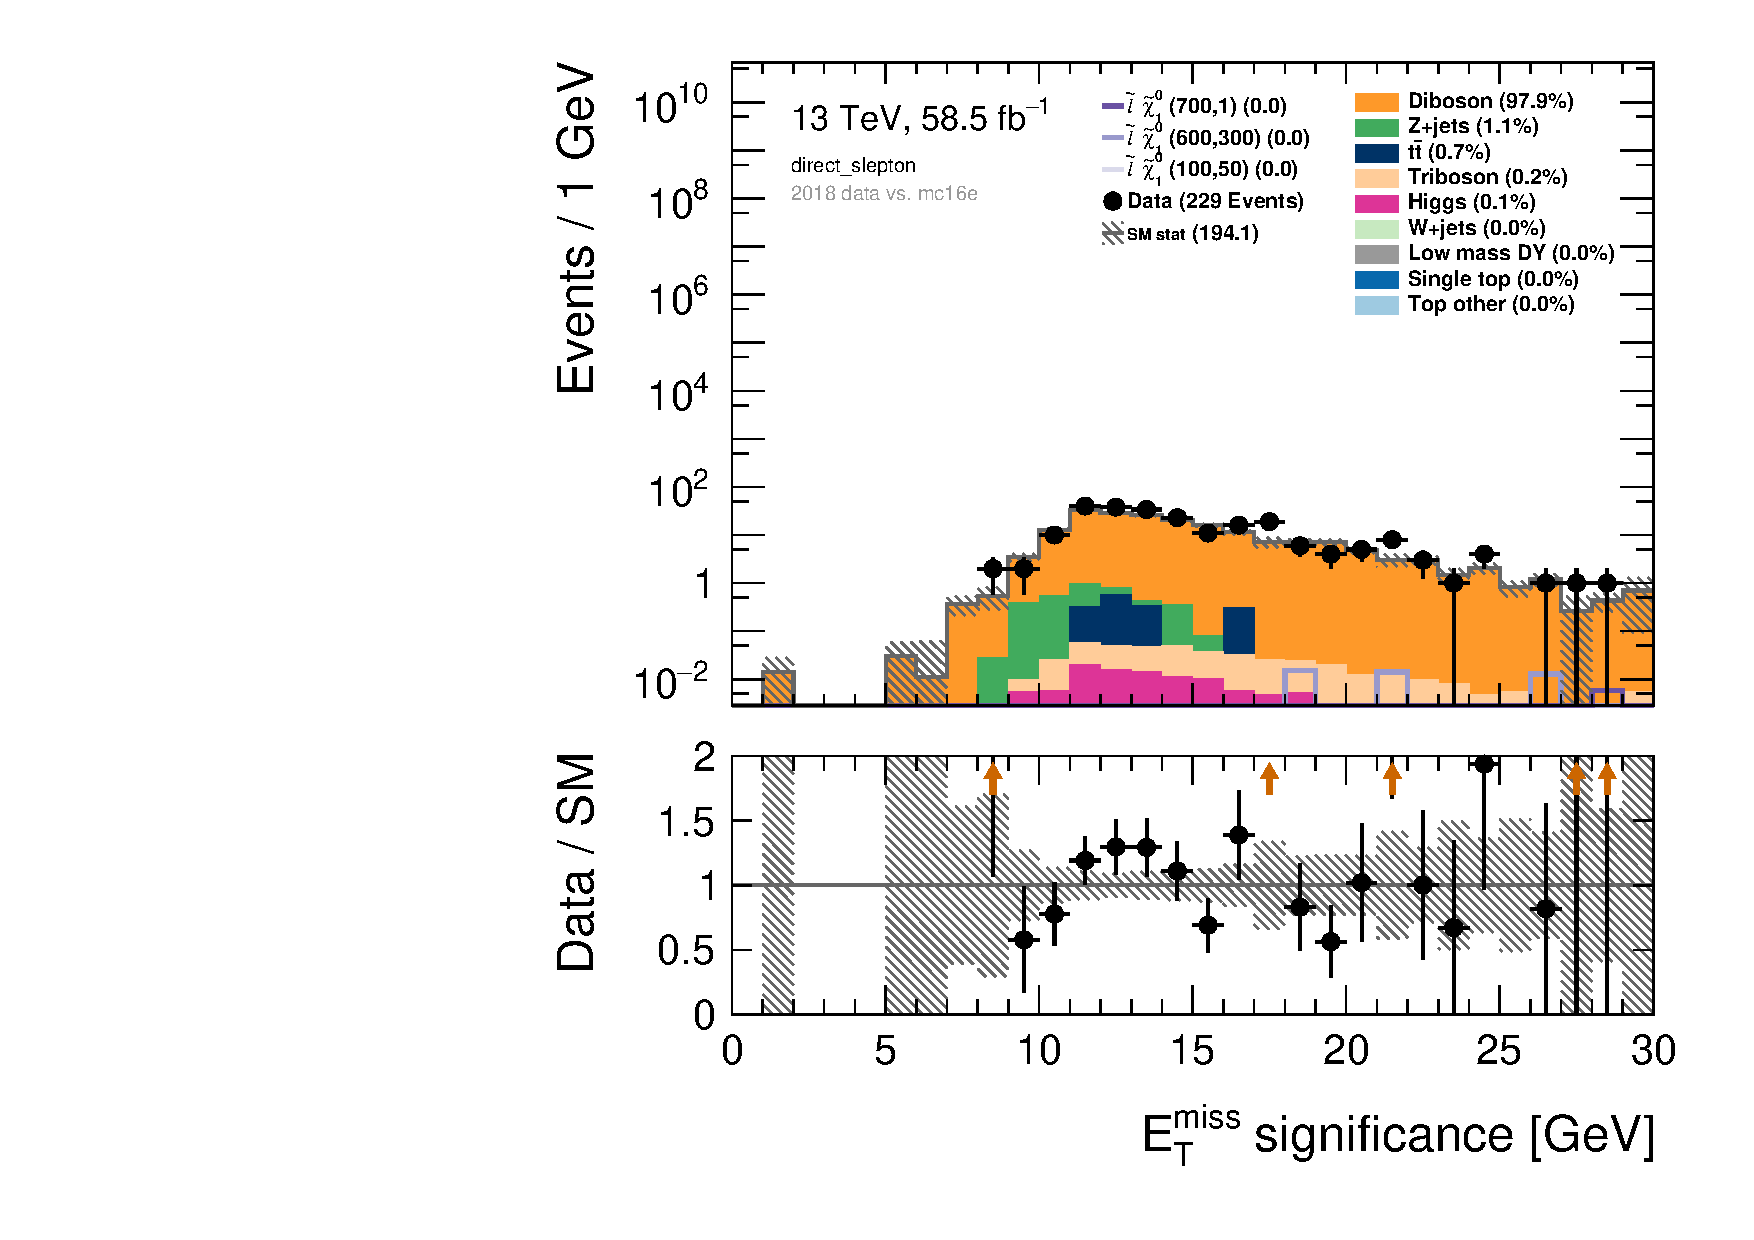
\includegraphics[width=\textwidth]{Figures/SlepSlep/CutAndCount/5thcut_1_mt2_100/hist1d_met_Sign_direct_slepton.pdf}
    \caption{Missing transverse energy significance}
    \label{fig:my_label}
    \end{subfigure}
    \caption{Plot of the four most important variables in direct slepton production with a cut on $m_{T_2} > 100$ GeV in addition to the previous cuts.}
    \label{fig:slepslep5th_1_cut}
\end{figure}


After adding all of the cuts mentioned above we can see that the signal almost no longer is present which is pretty bad when we want to see if the data follows the signal or the background. Since this isn't working that well, we are going to try to see if cuts found by ML is a better solution. 

\end{comment}















\begin{comment}


\begin{figure}[H]
%\begin{minipage}{2\textwidth}
%\begin{adjustwidth}{-3cm}{-3cm}
\centering
%\advance\leftskip-4cm 
%\advance\rightskip-4cm 
    \begin{subfigure}[t!]{0.49\textwidth}
        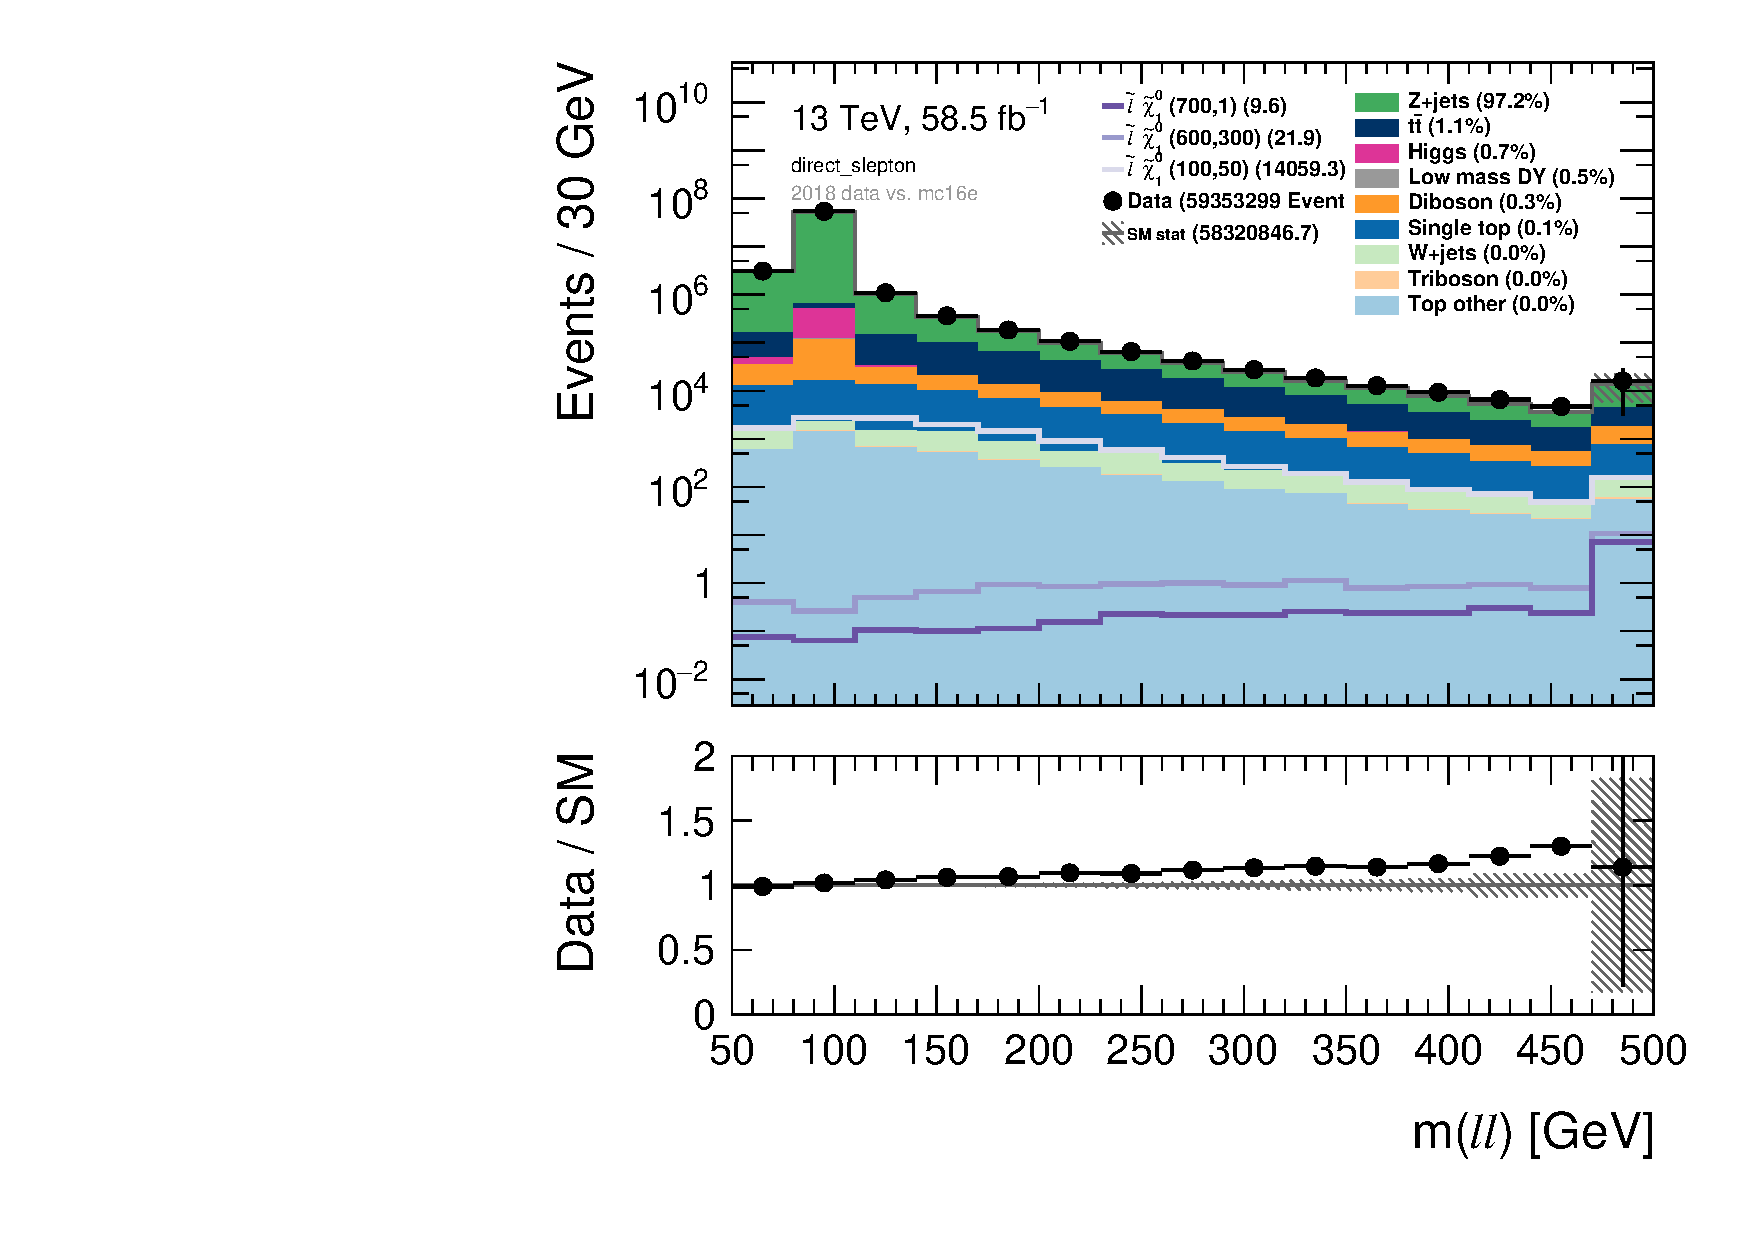
\includegraphics[width=\textwidth]{Figures/SlepSlep/CutAndCount/1stcut_2L+OS/hist1d_mll_direct_slepton.pdf}
%    \caption{Caption}
    \label{fig:my_label}
    \end{subfigure}
    \begin{subfigure}[t!]{0.49\textwidth}
        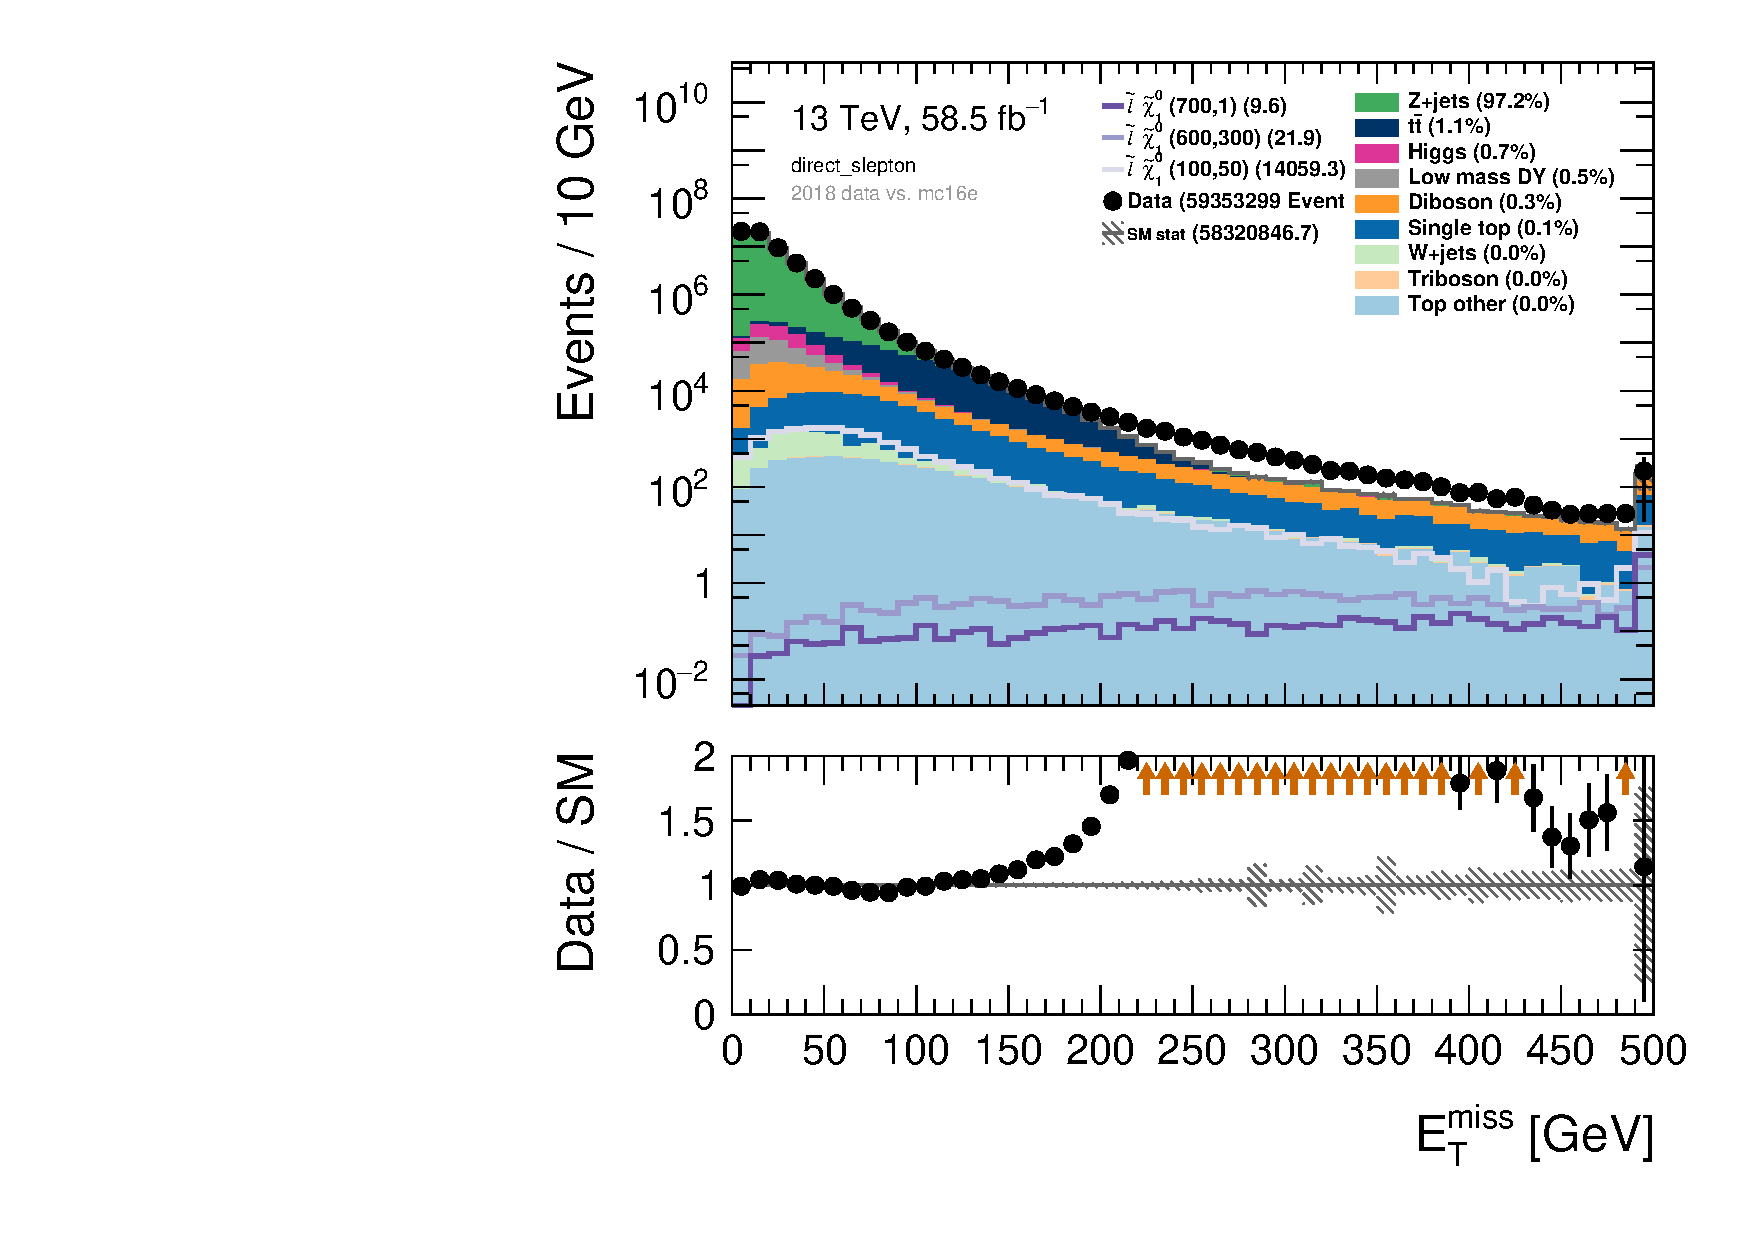
\includegraphics[width=\textwidth]{Figures/SlepSlep/CutAndCount/1stcut_2L+OS/hist1d_met_Et_direct_slepton.pdf}
 %   \caption{Caption}
    \label{fig:my_label}
    \end{subfigure}
    \\
    \begin{subfigure}[t!]{0.49\textwidth}
        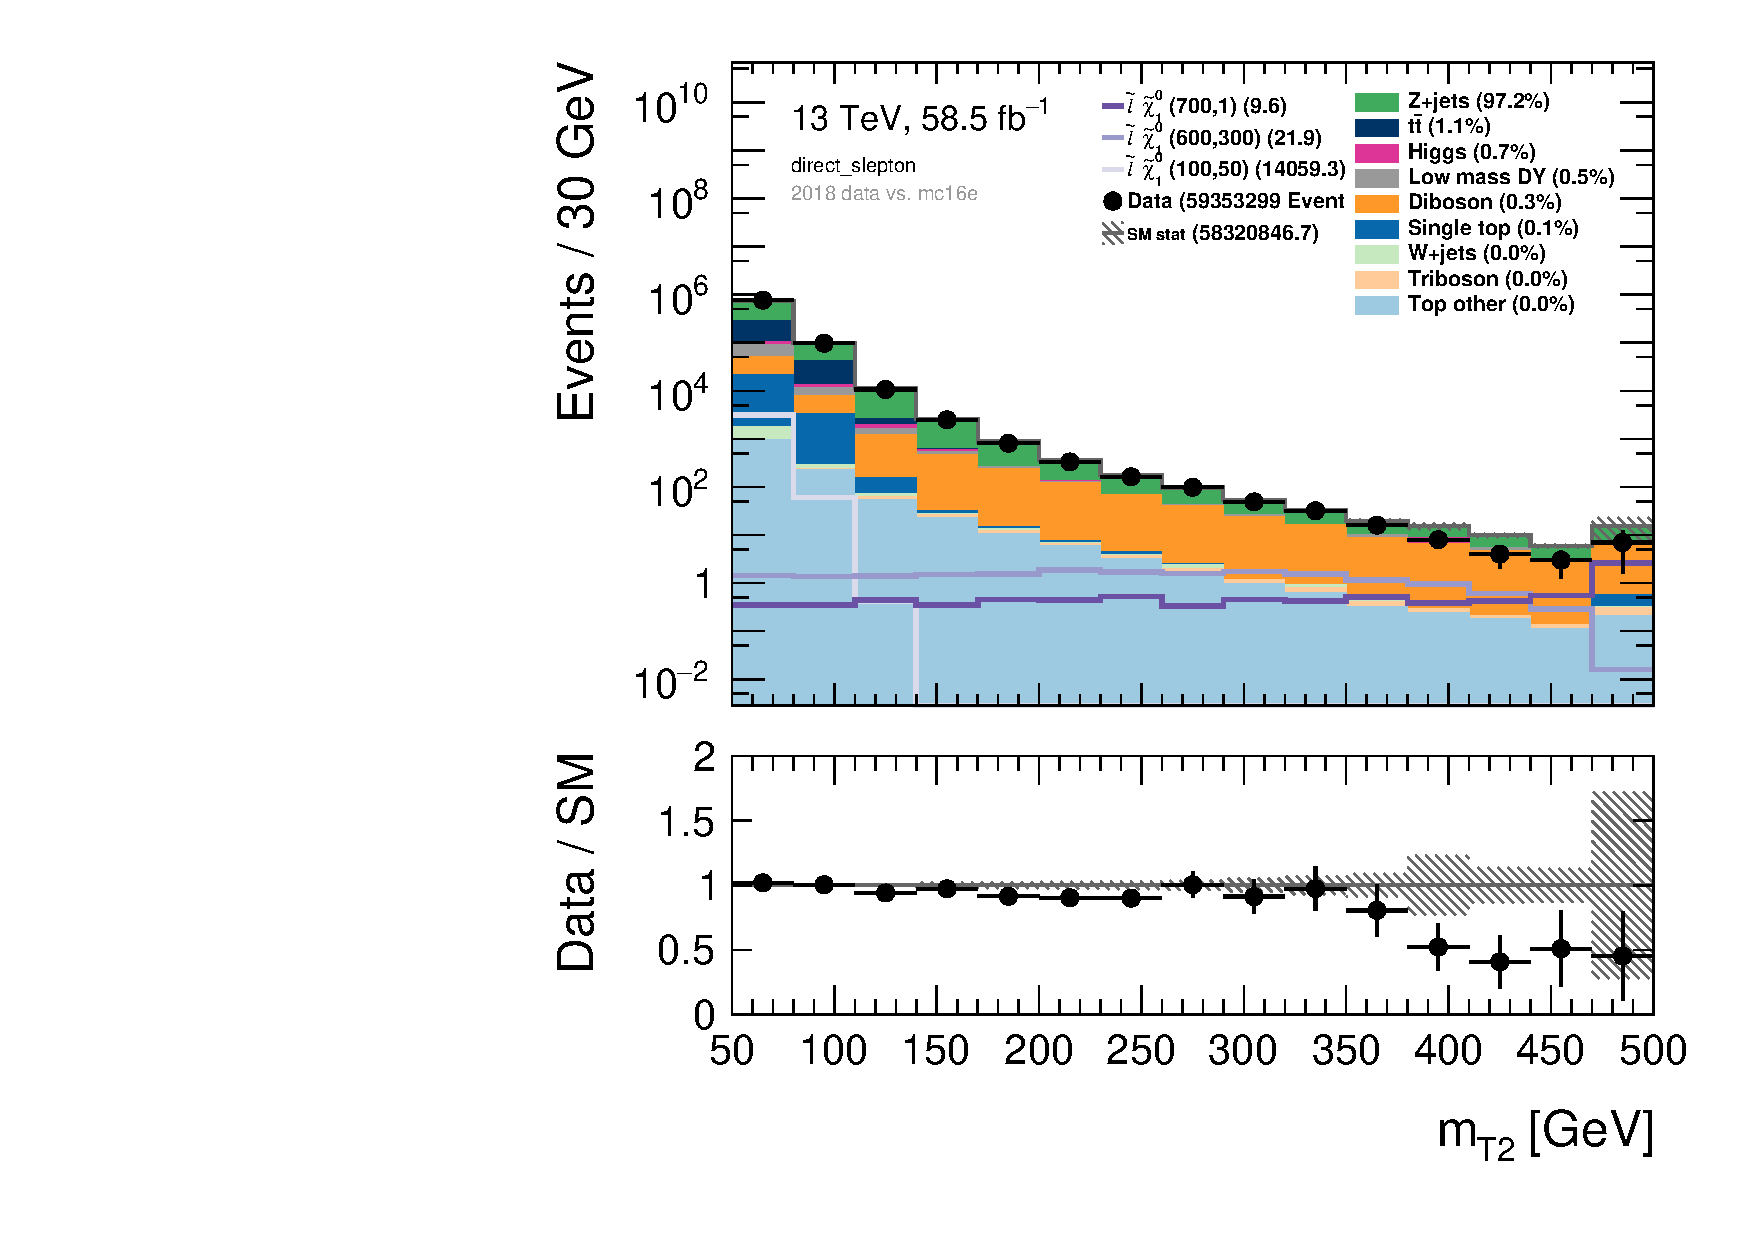
\includegraphics[width=\textwidth]{Figures/SlepSlep/CutAndCount/1stcut_2L+OS/hist1d_mt2_direct_slepton.pdf}
  %  \caption{Caption}
    \label{fig:my_label}
    \end{subfigure}
    \begin{subfigure}[t!]{0.49\textwidth}
        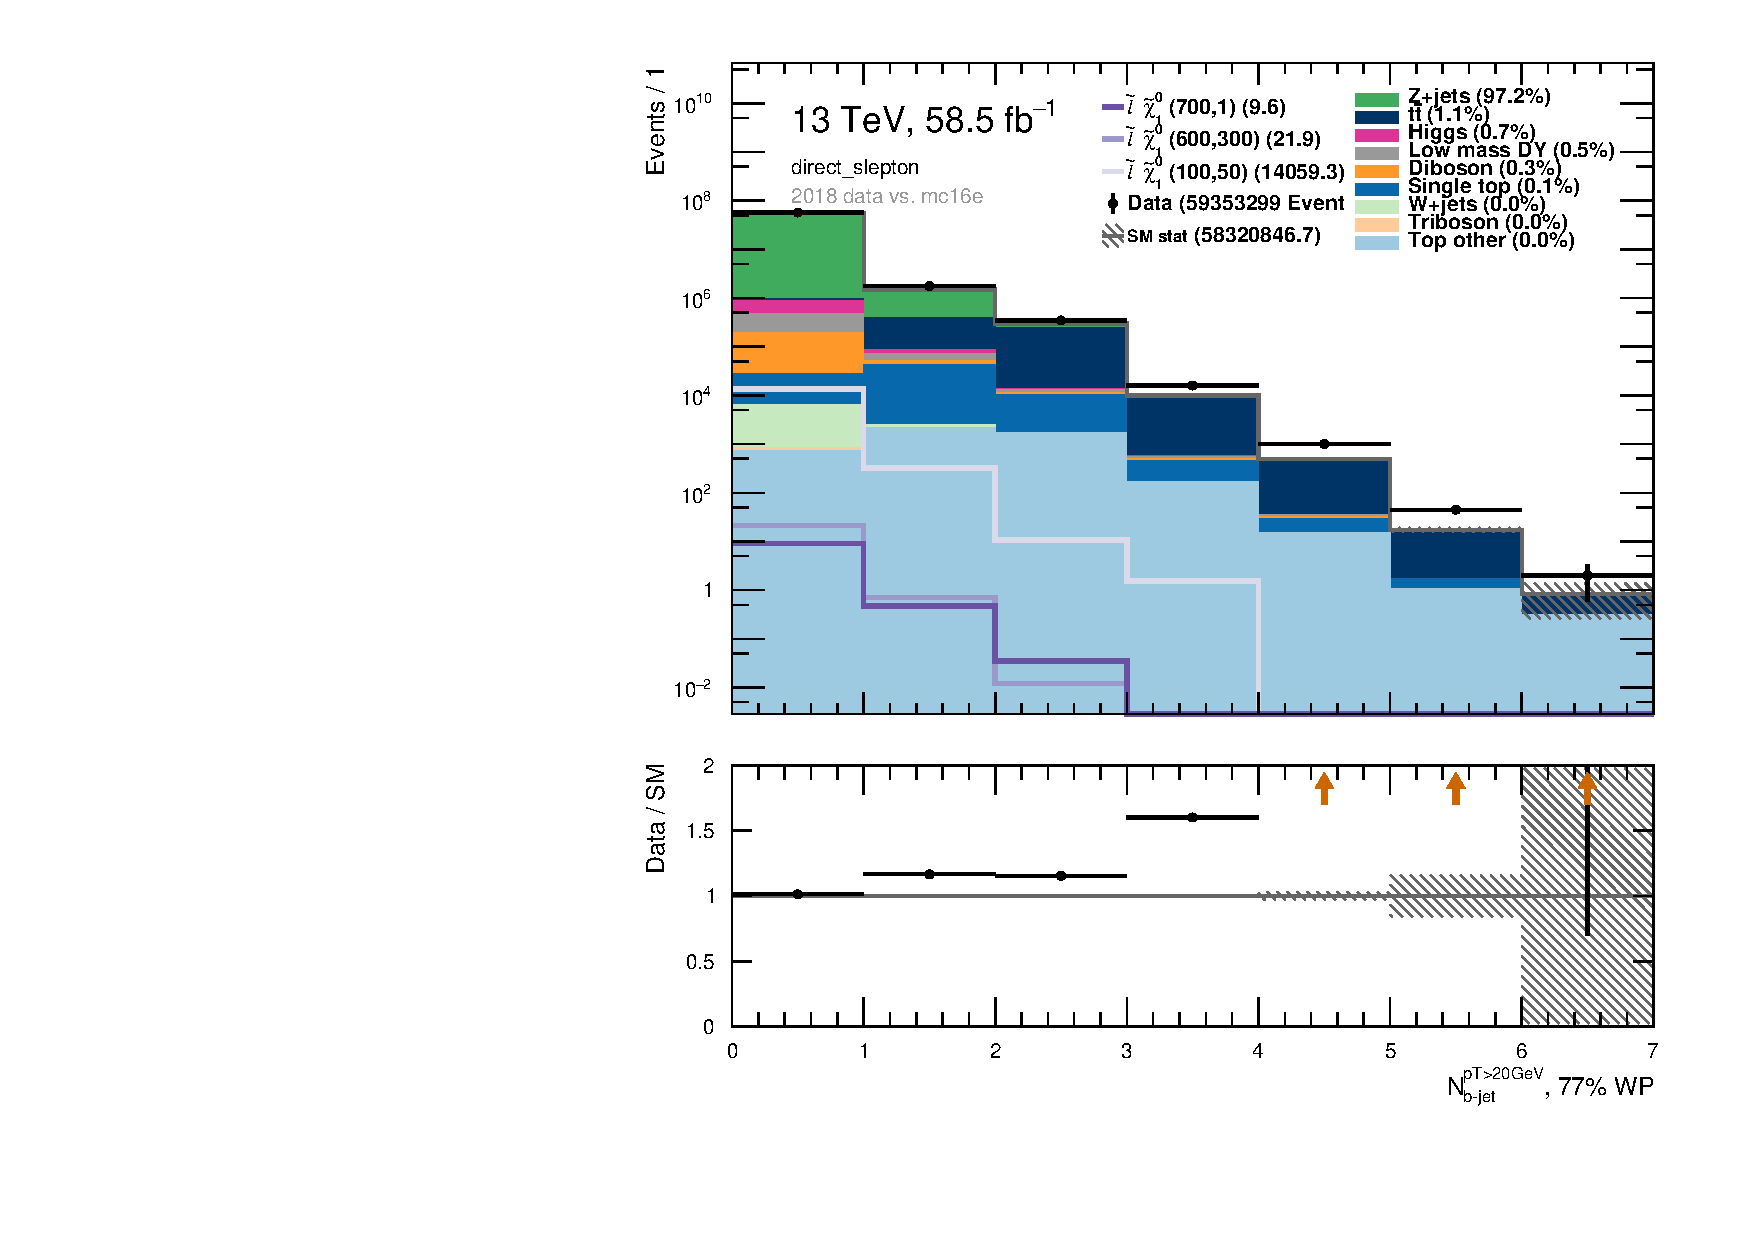
\includegraphics[width=\textwidth]{Figures/SlepSlep/CutAndCount/1stcut_2L+OS/hist1d_nBJet20_MV2c10_FixedCutBEff_77_direct_slepton.pdf}
  %  \caption{Caption}
    \label{fig:my_label}
    \end{subfigure}
    \\
    \begin{subfigure}[t!]{0.49\textwidth}
        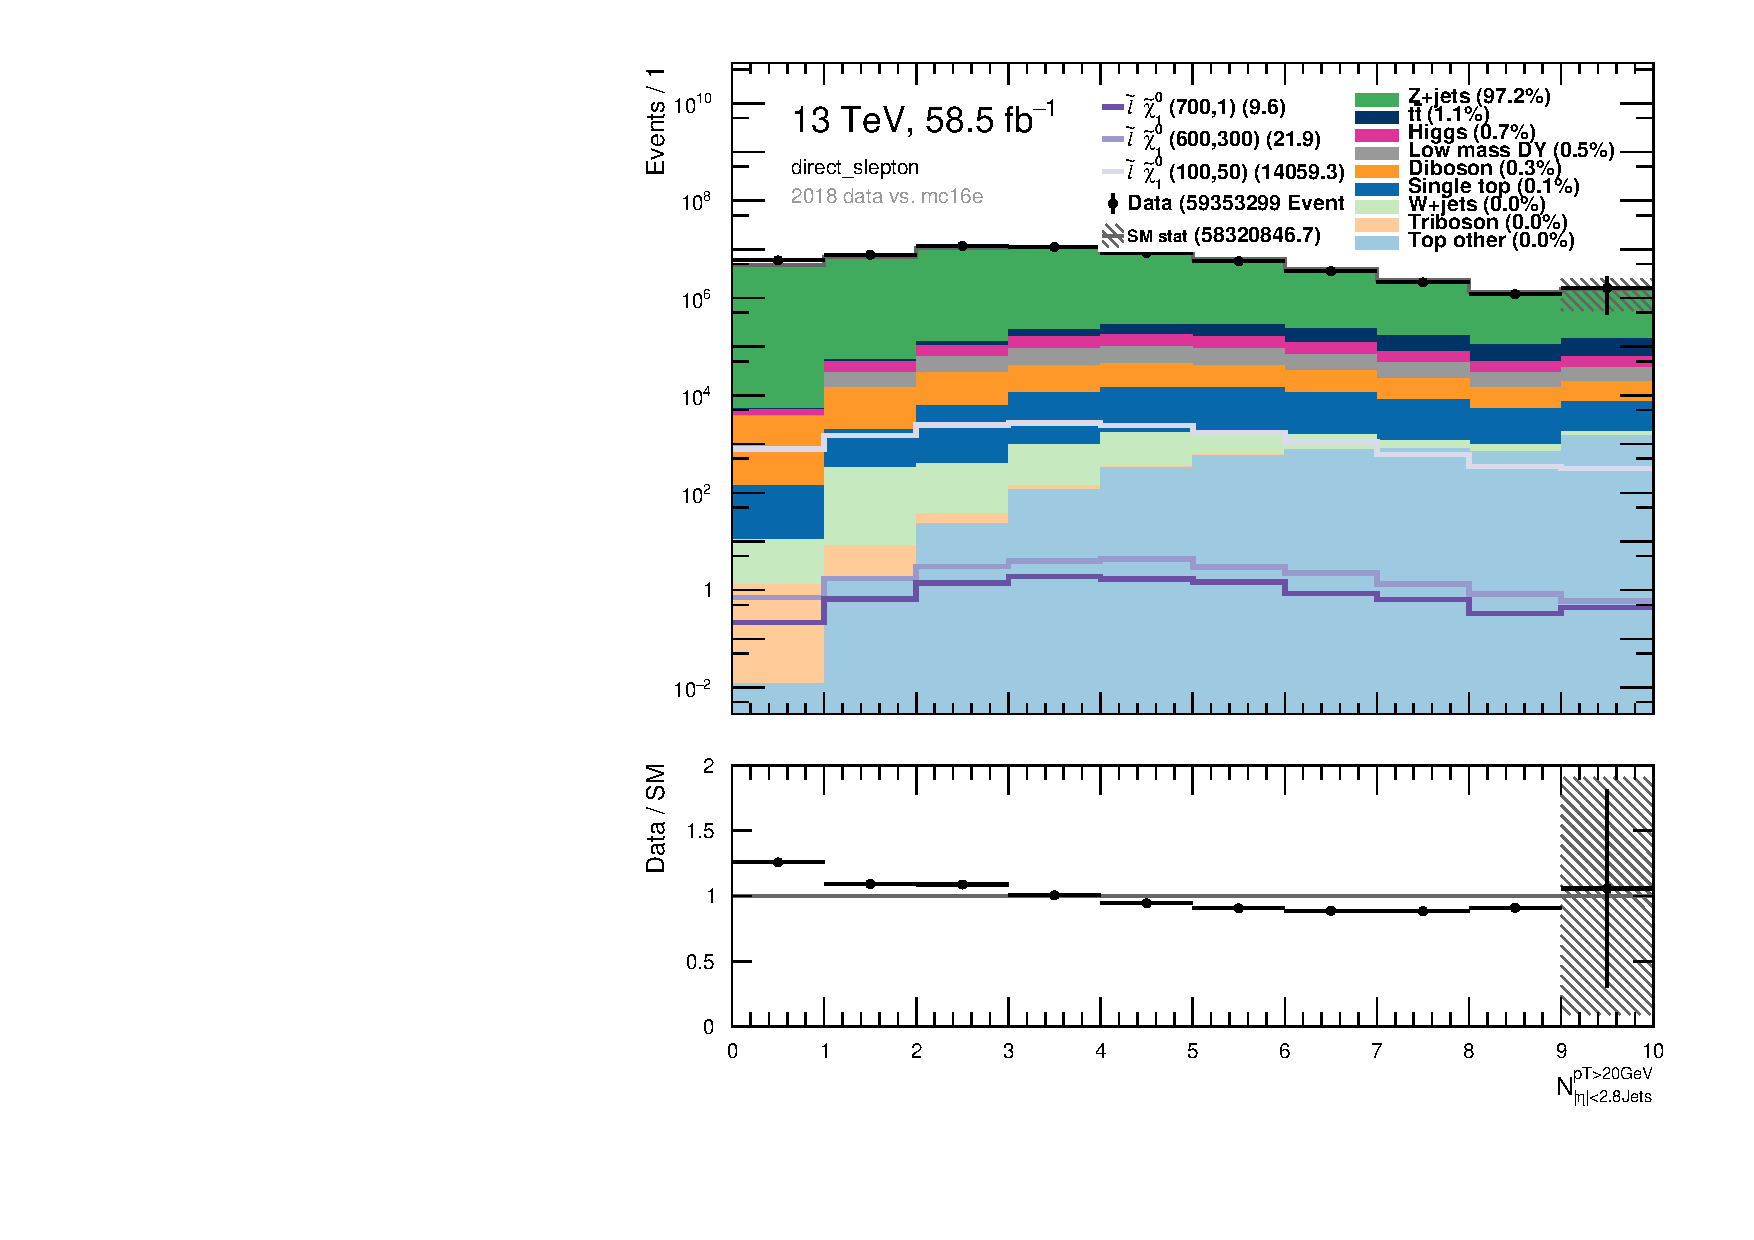
\includegraphics[width=\textwidth]{Figures/SlepSlep/CutAndCount/1stcut_2L+OS/hist1d_nJet20_direct_slepton.pdf}
%    \caption{Caption}
    \label{fig:my_label}
    \end{subfigure}
    \begin{subfigure}[t!]{0.49\textwidth}
        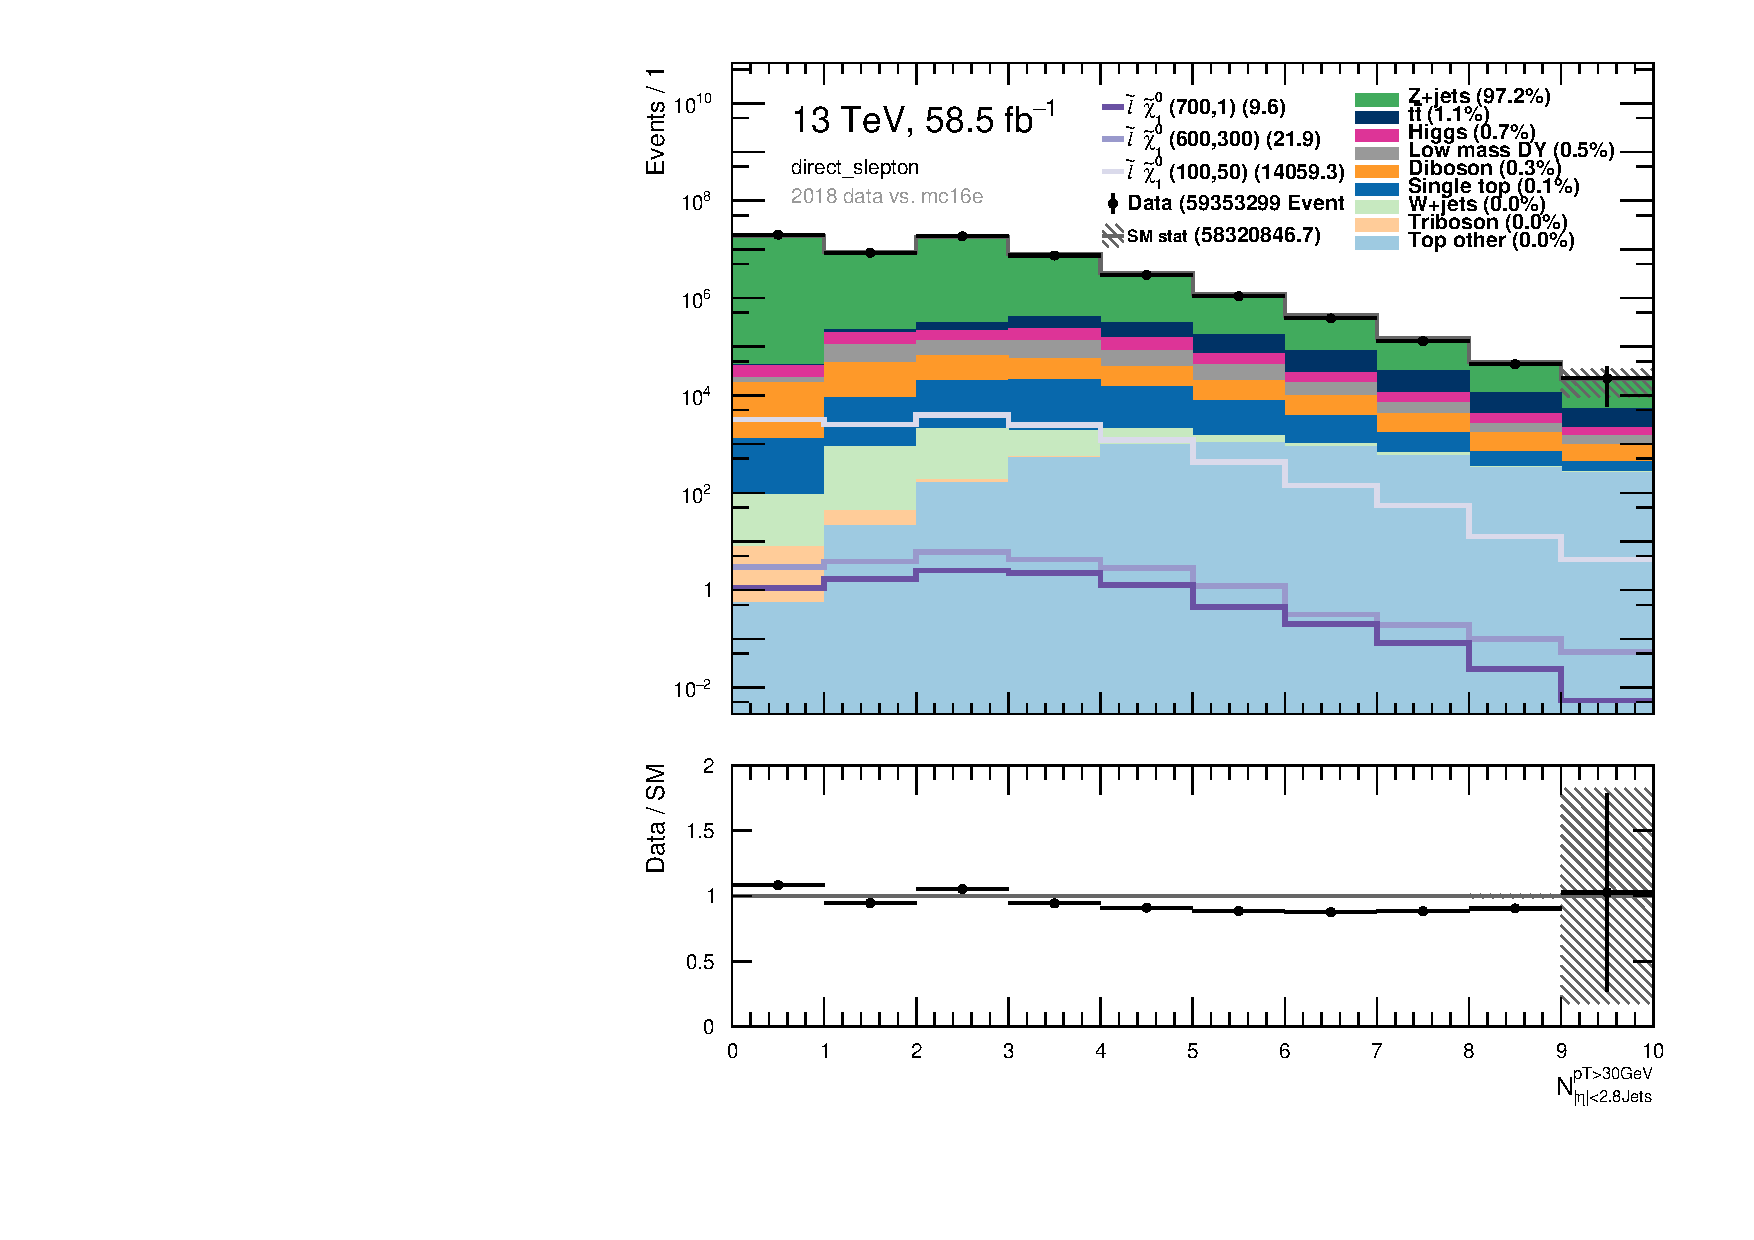
\includegraphics[width=\textwidth]{Figures/SlepSlep/CutAndCount/1stcut_2L+OS/hist1d_nJet30_direct_slepton.pdf}
 %   \caption{Caption}
    \label{fig:my_label}
    \end{subfigure}
\end{figure}

\begin{figure}[H]
%\begin{minipage}{2\textwidth}
%\begin{adjustwidth}{-3cm}{-3cm}
\centering
%\advance\leftskip-4cm 
%\advance\rightskip-4cm 
    \begin{subfigure}[t!]{0.49\textwidth}
        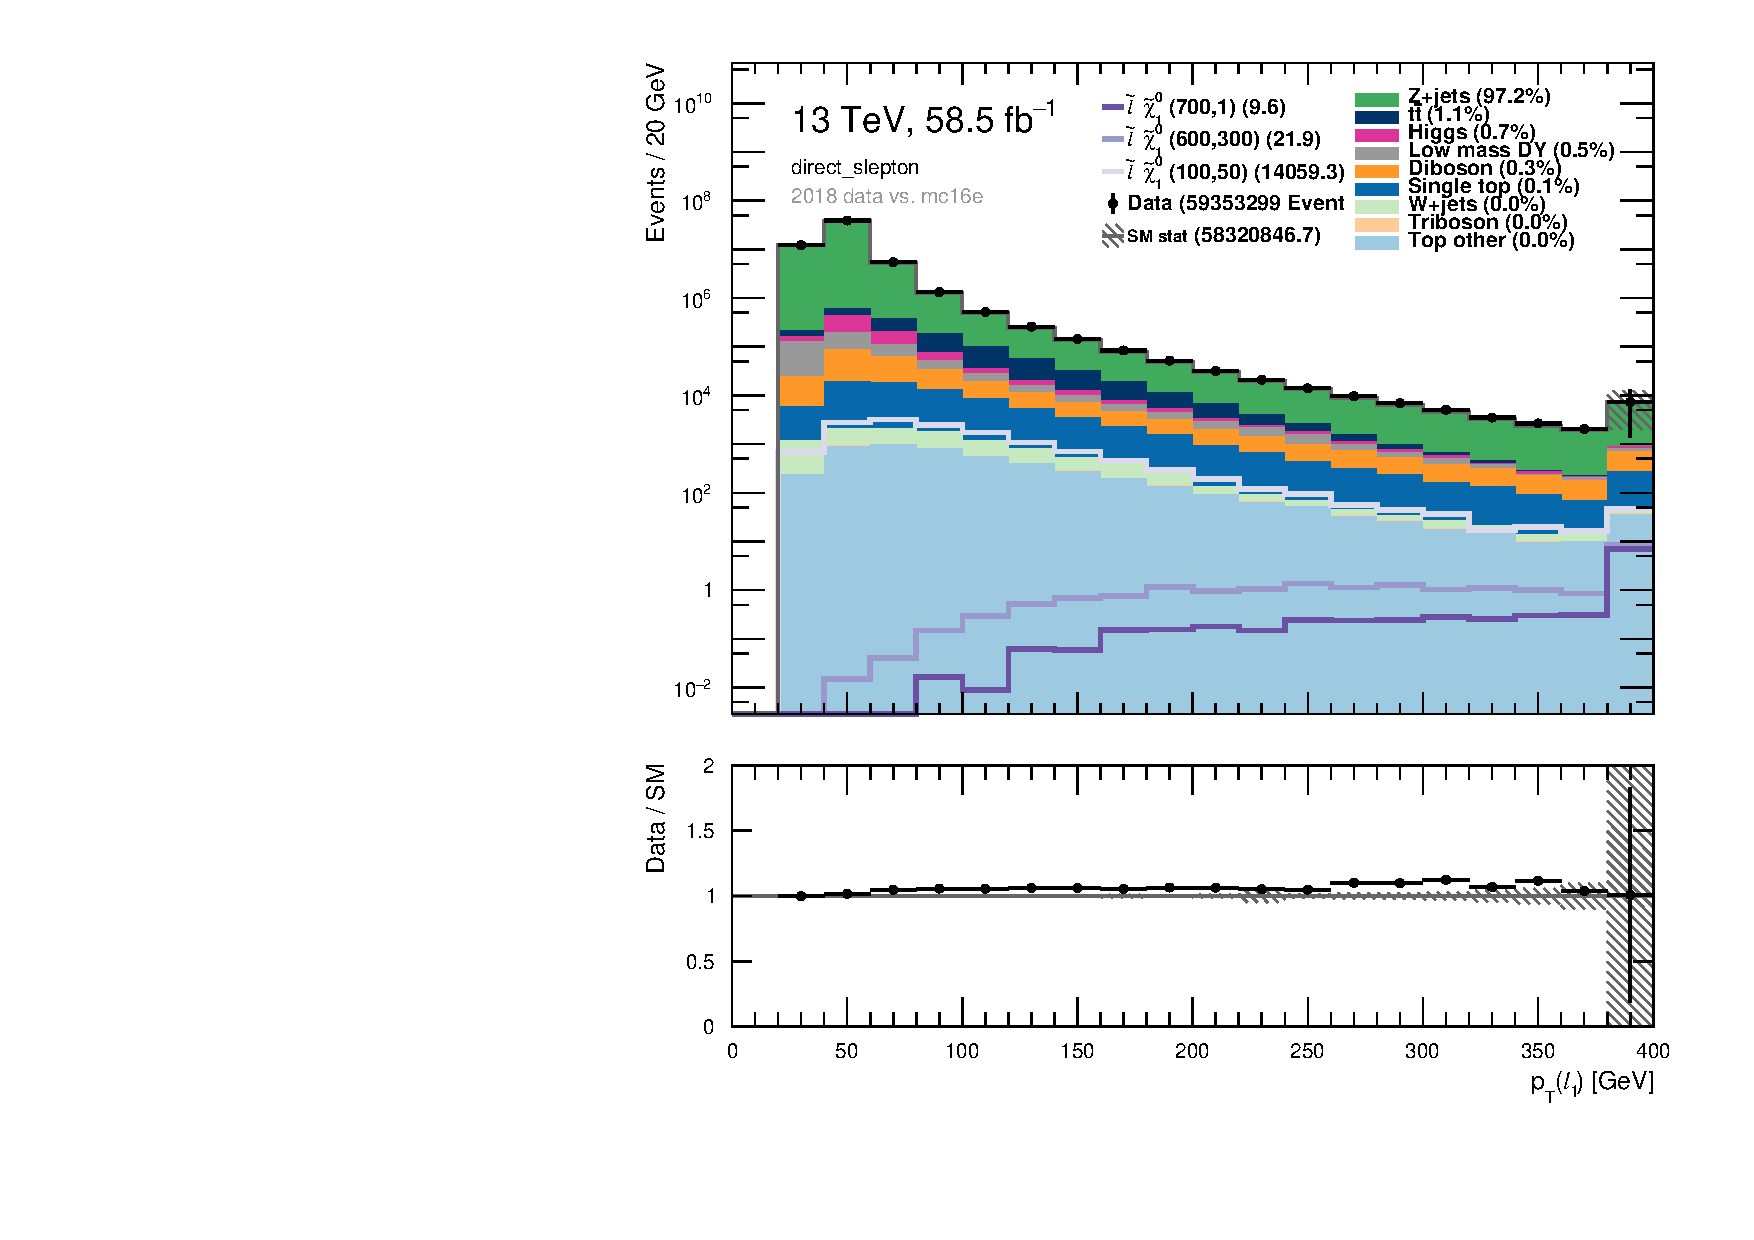
\includegraphics[width=\textwidth]{Figures/SlepSlep/CutAndCount/1stcut_2L+OS/hist1d_lepPt[0]_direct_slepton.pdf}
%    \caption{Caption}
    \label{fig:my_label}
    \end{subfigure}
    \begin{subfigure}[t!]{0.49\textwidth}
        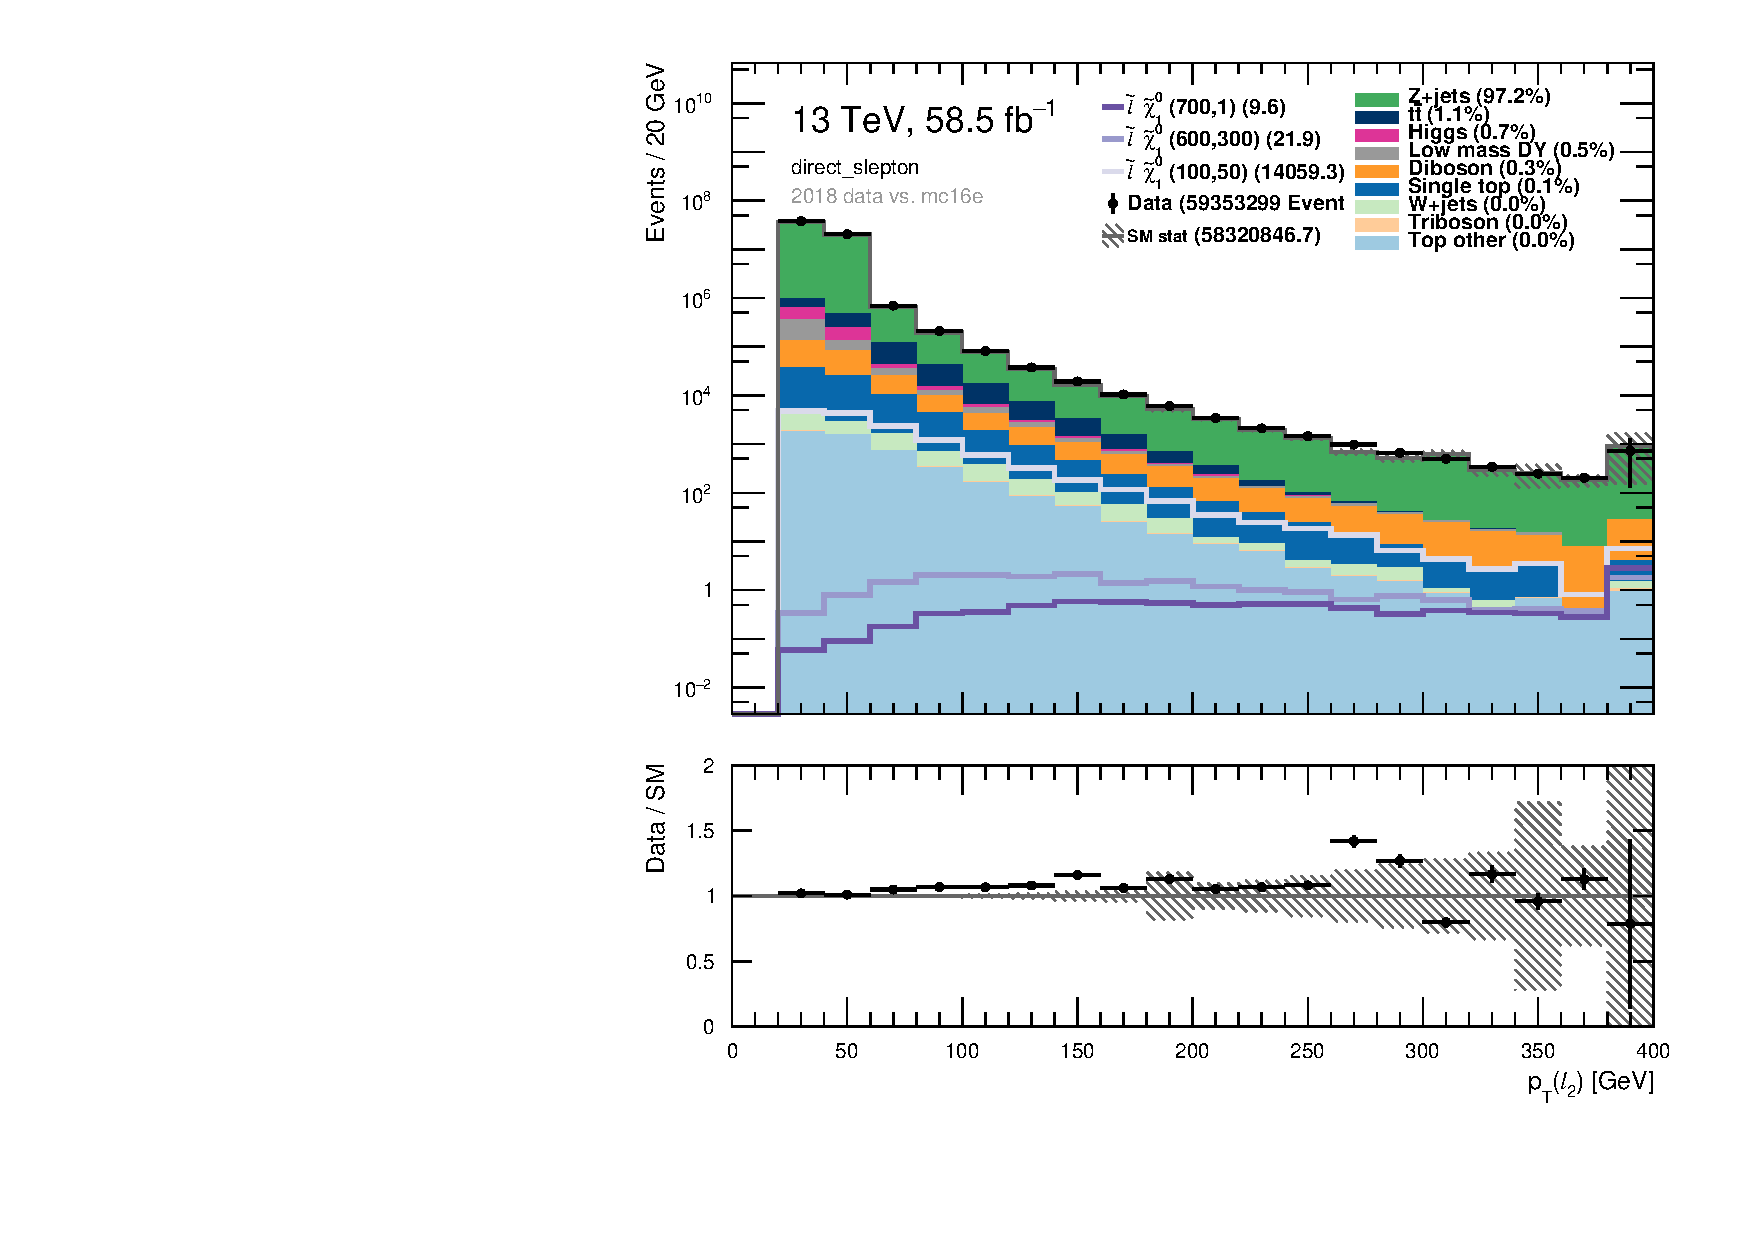
\includegraphics[width=\textwidth]{Figures/SlepSlep/CutAndCount/1stcut_2L+OS/hist1d_lepPt[1]_direct_slepton.pdf}
 %   \caption{Caption}
    \\
    \label{fig:my_label}
    \end{subfigure}
    \begin{subfigure}[t!]{0.49\textwidth}
        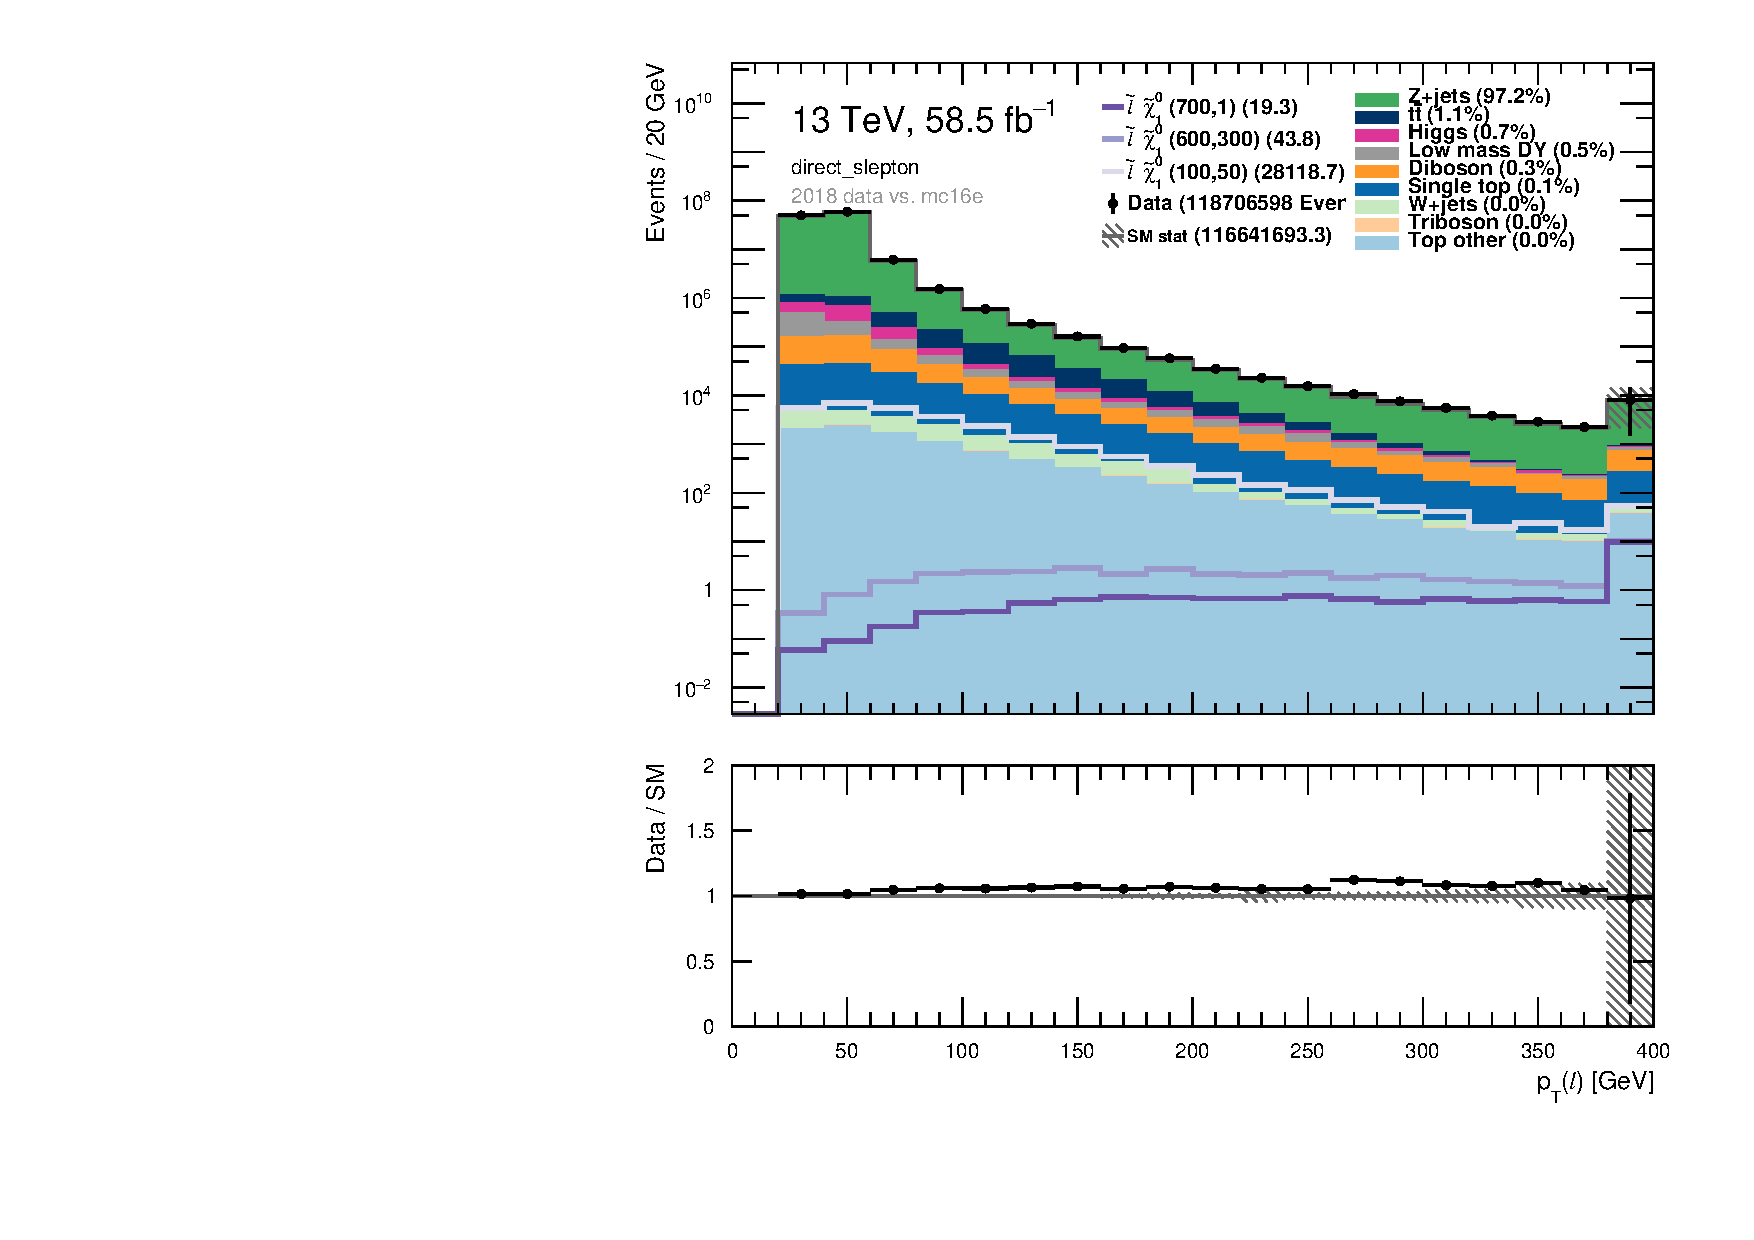
\includegraphics[width=\textwidth]{Figures/SlepSlep/CutAndCount/1stcut_2L+OS/hist1d_lepPt_direct_slepton.pdf}
  %  \caption{Caption}
    \label{fig:my_label}
    \end{subfigure}
    \begin{subfigure}[t!]{0.49\textwidth}
        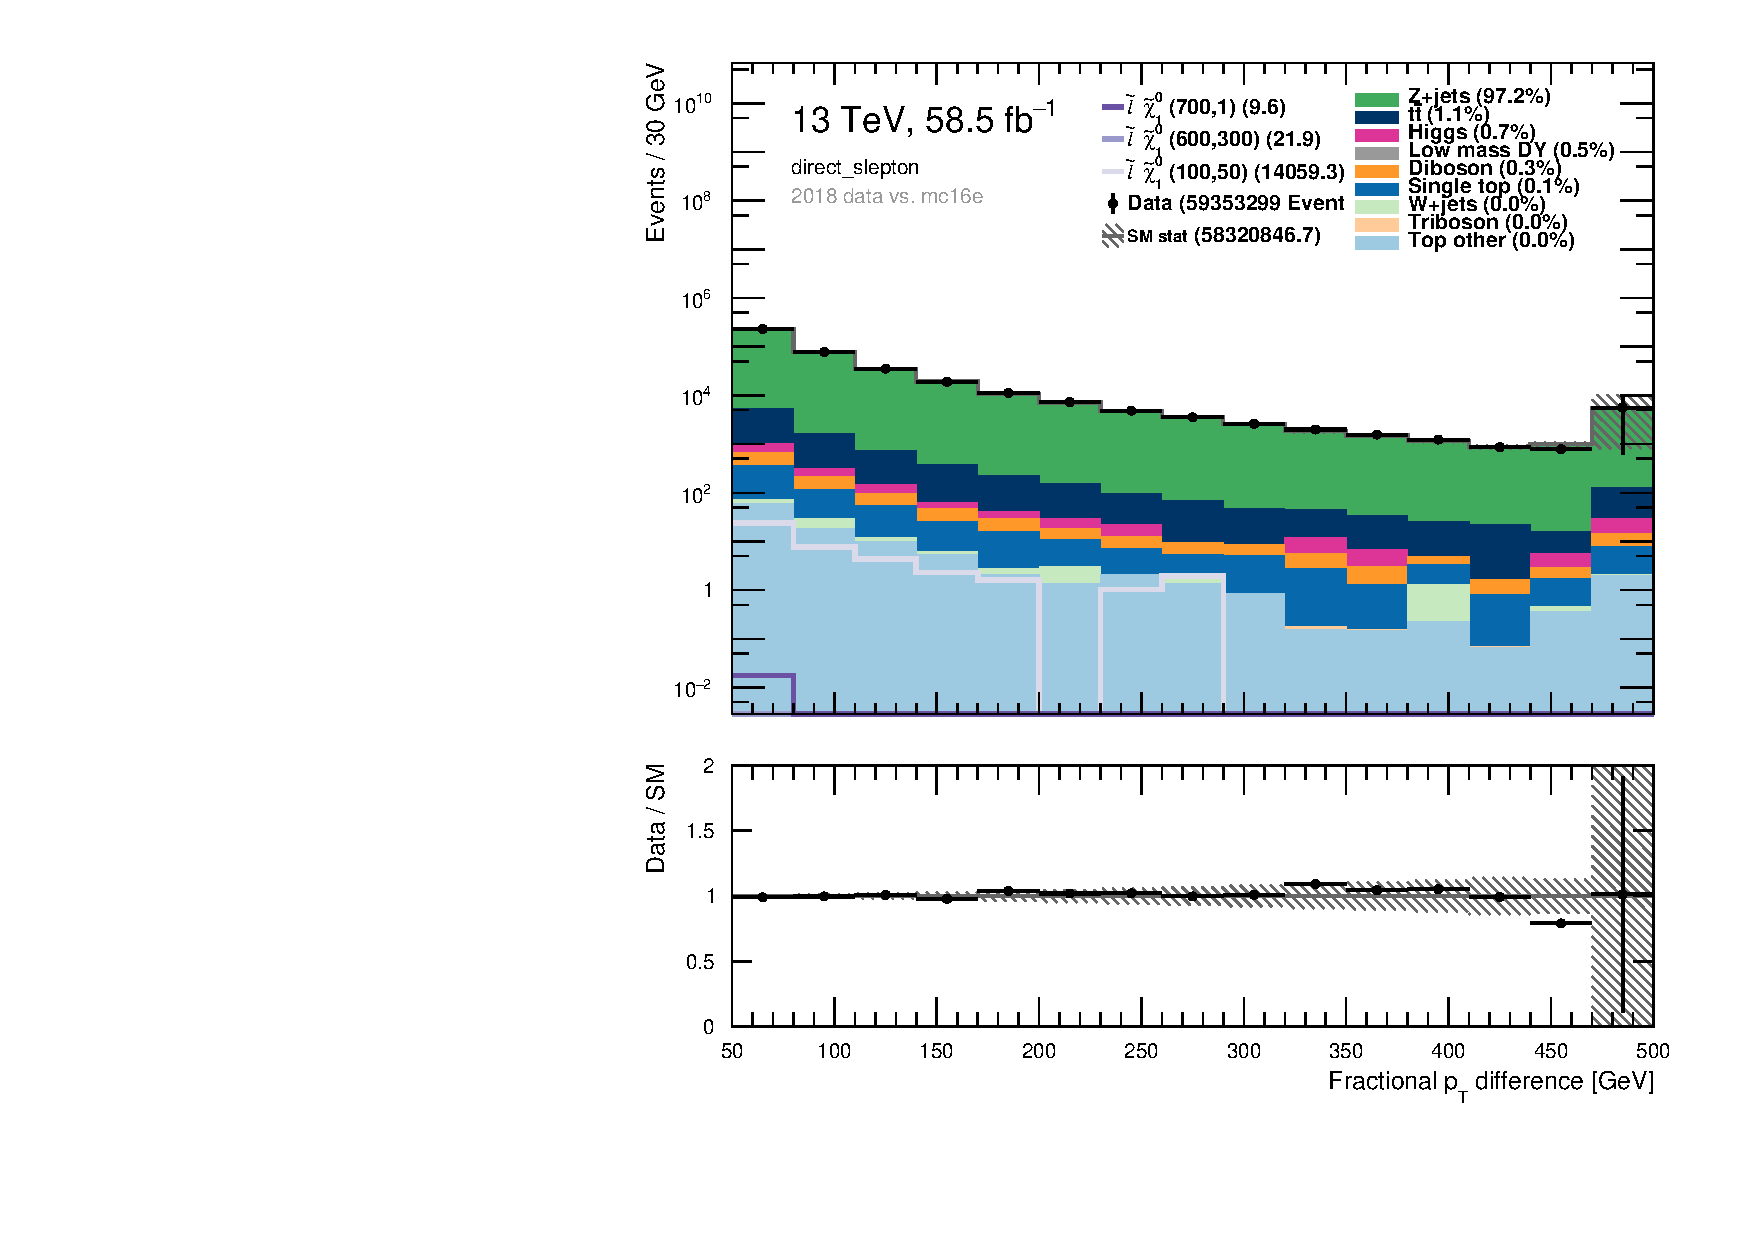
\includegraphics[width=\textwidth]{Figures/SlepSlep/CutAndCount/1stcut_2L+OS/hist1d_pTdiff_direct_slepton.pdf}
%    \caption{Caption}
    \\
    \label{fig:my_label}
    \end{subfigure}
    \begin{subfigure}[t!]{0.49\textwidth}
        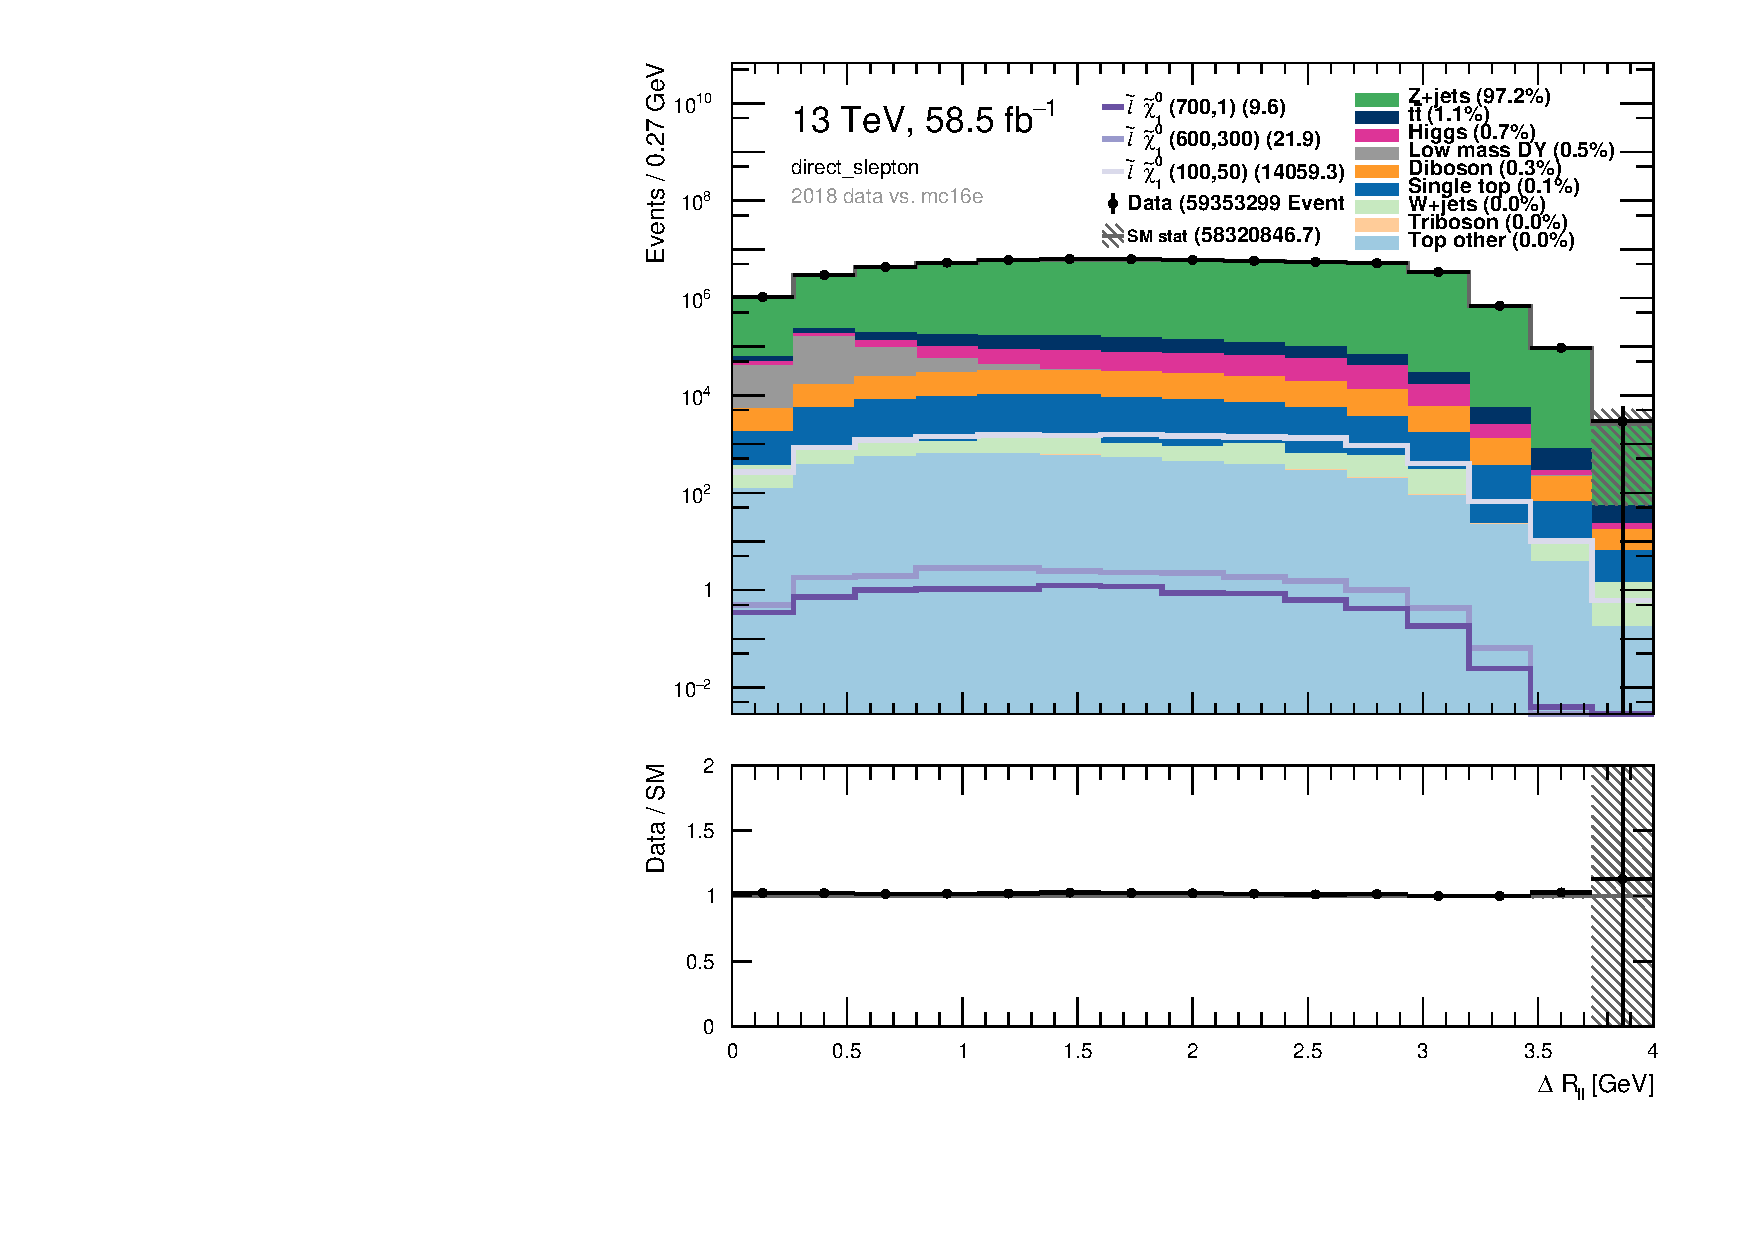
\includegraphics[width=\textwidth]{Figures/SlepSlep/CutAndCount/1stcut_2L+OS/hist1d_deltaRll_direct_slepton.pdf}
 %   \caption{Caption}
    \label{fig:my_label}
    \end{subfigure}
    \begin{subfigure}[t!]{0.49\textwidth}
        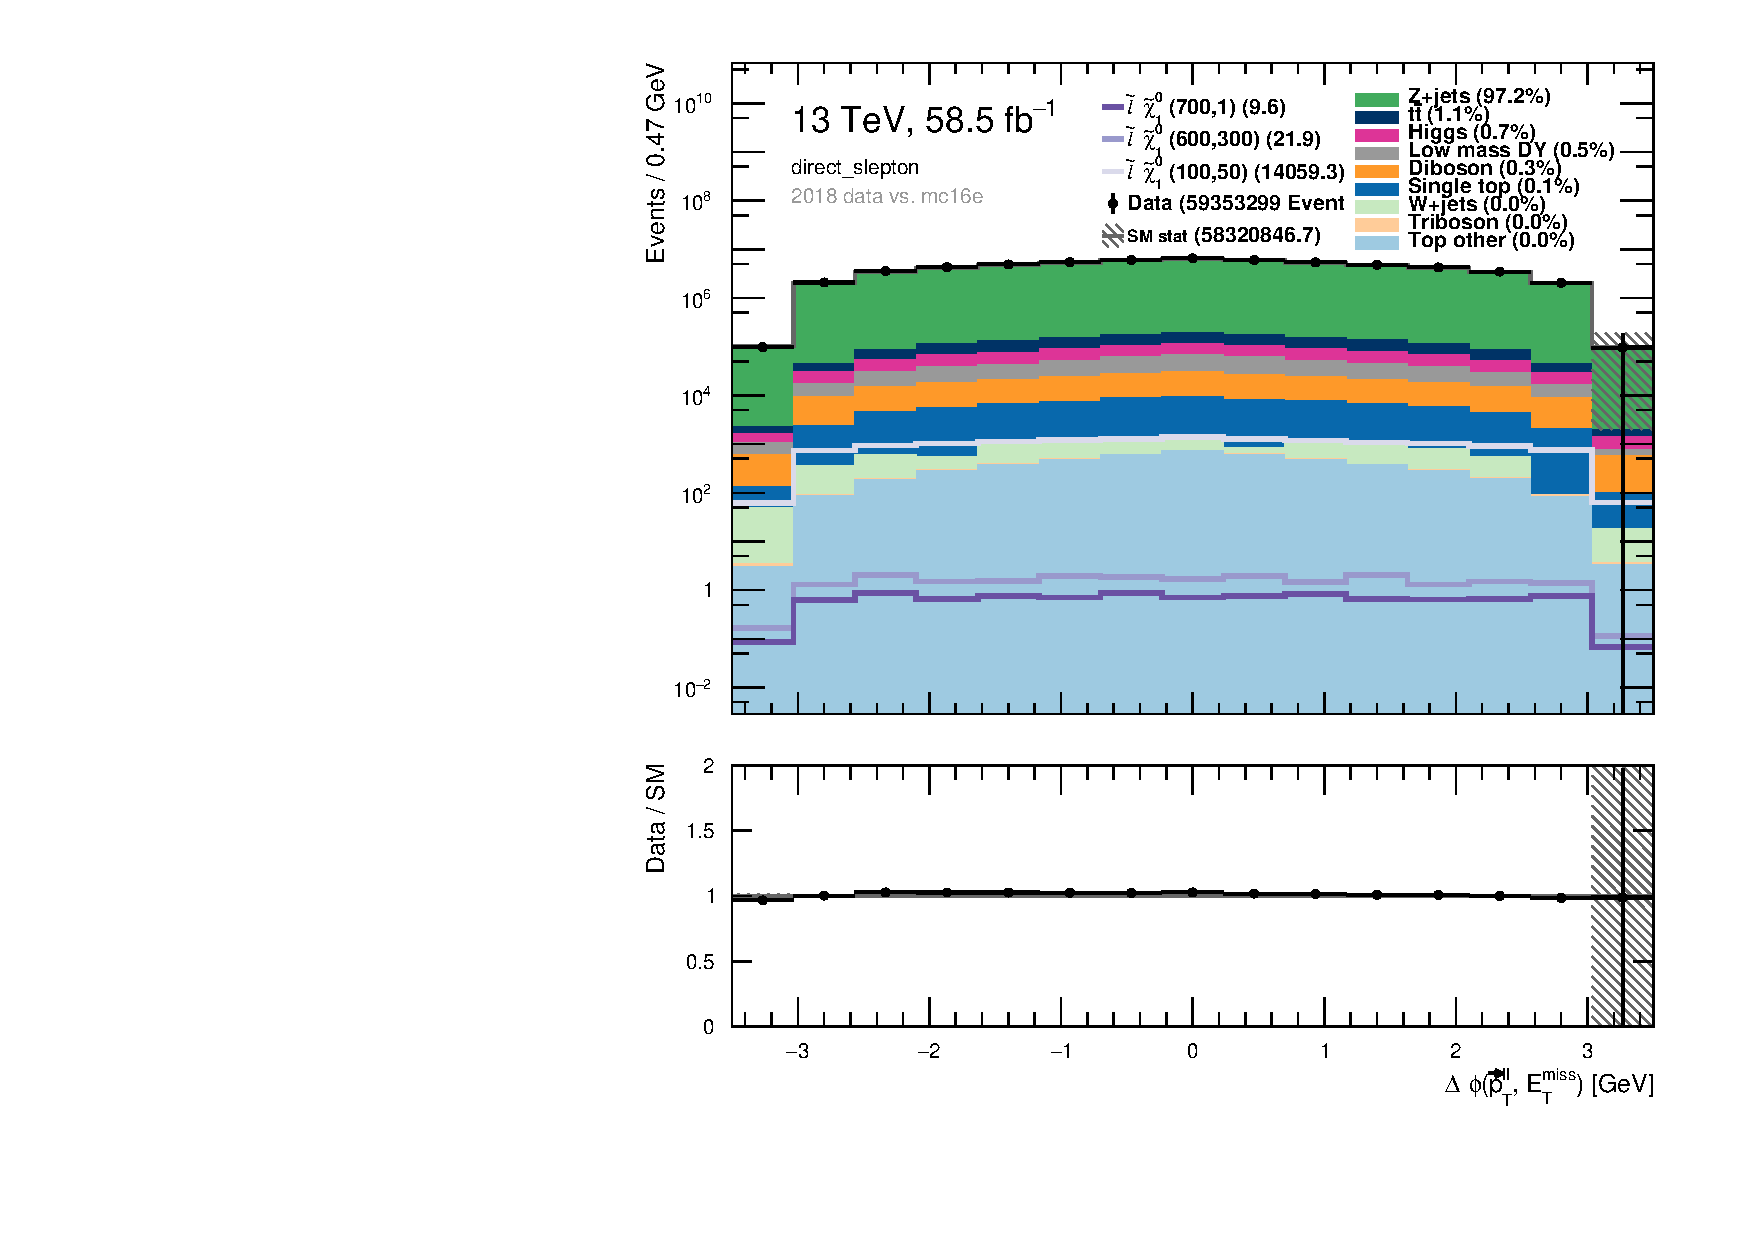
\includegraphics[width=\textwidth]{Figures/SlepSlep/CutAndCount/1stcut_2L+OS/hist1d_deltaPhi_direct_slepton.pdf}
  %  \caption{Caption}
    \label{fig:my_label}
    \end{subfigure}
\end{figure}

\begin{figure}[H]
%\begin{minipage}{2\textwidth}
%\begin{adjustwidth}{-3cm}{-3cm}
\centering
    \begin{subfigure}[t!]{0.49\textwidth}
        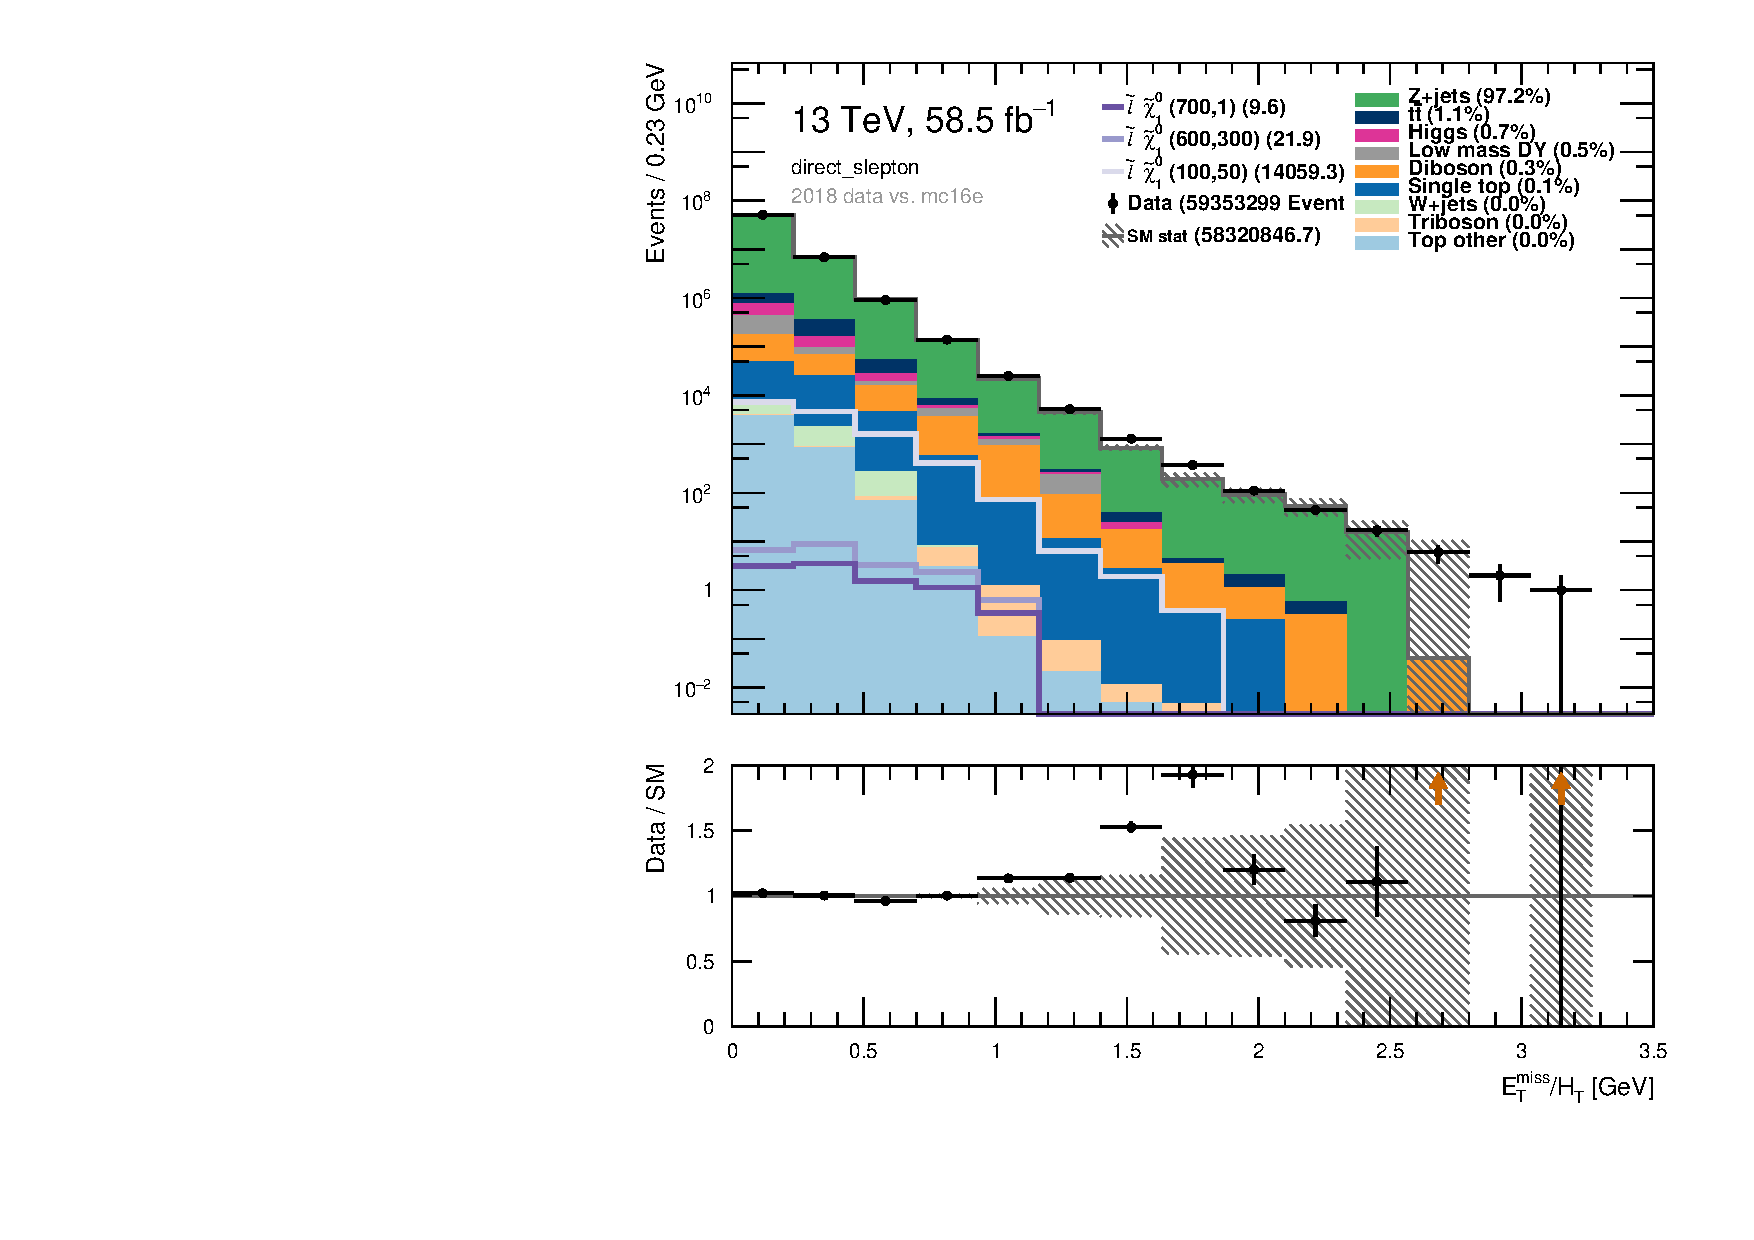
\includegraphics[width=\textwidth]{Figures/SlepSlep/CutAndCount/1stcut_2L+OS/hist1d_met_HT_direct_slepton.pdf}
%    \caption{Caption}
    \label{fig:my_label}
    \end{subfigure}
    \begin{subfigure}[t!]{0.49\textwidth}
        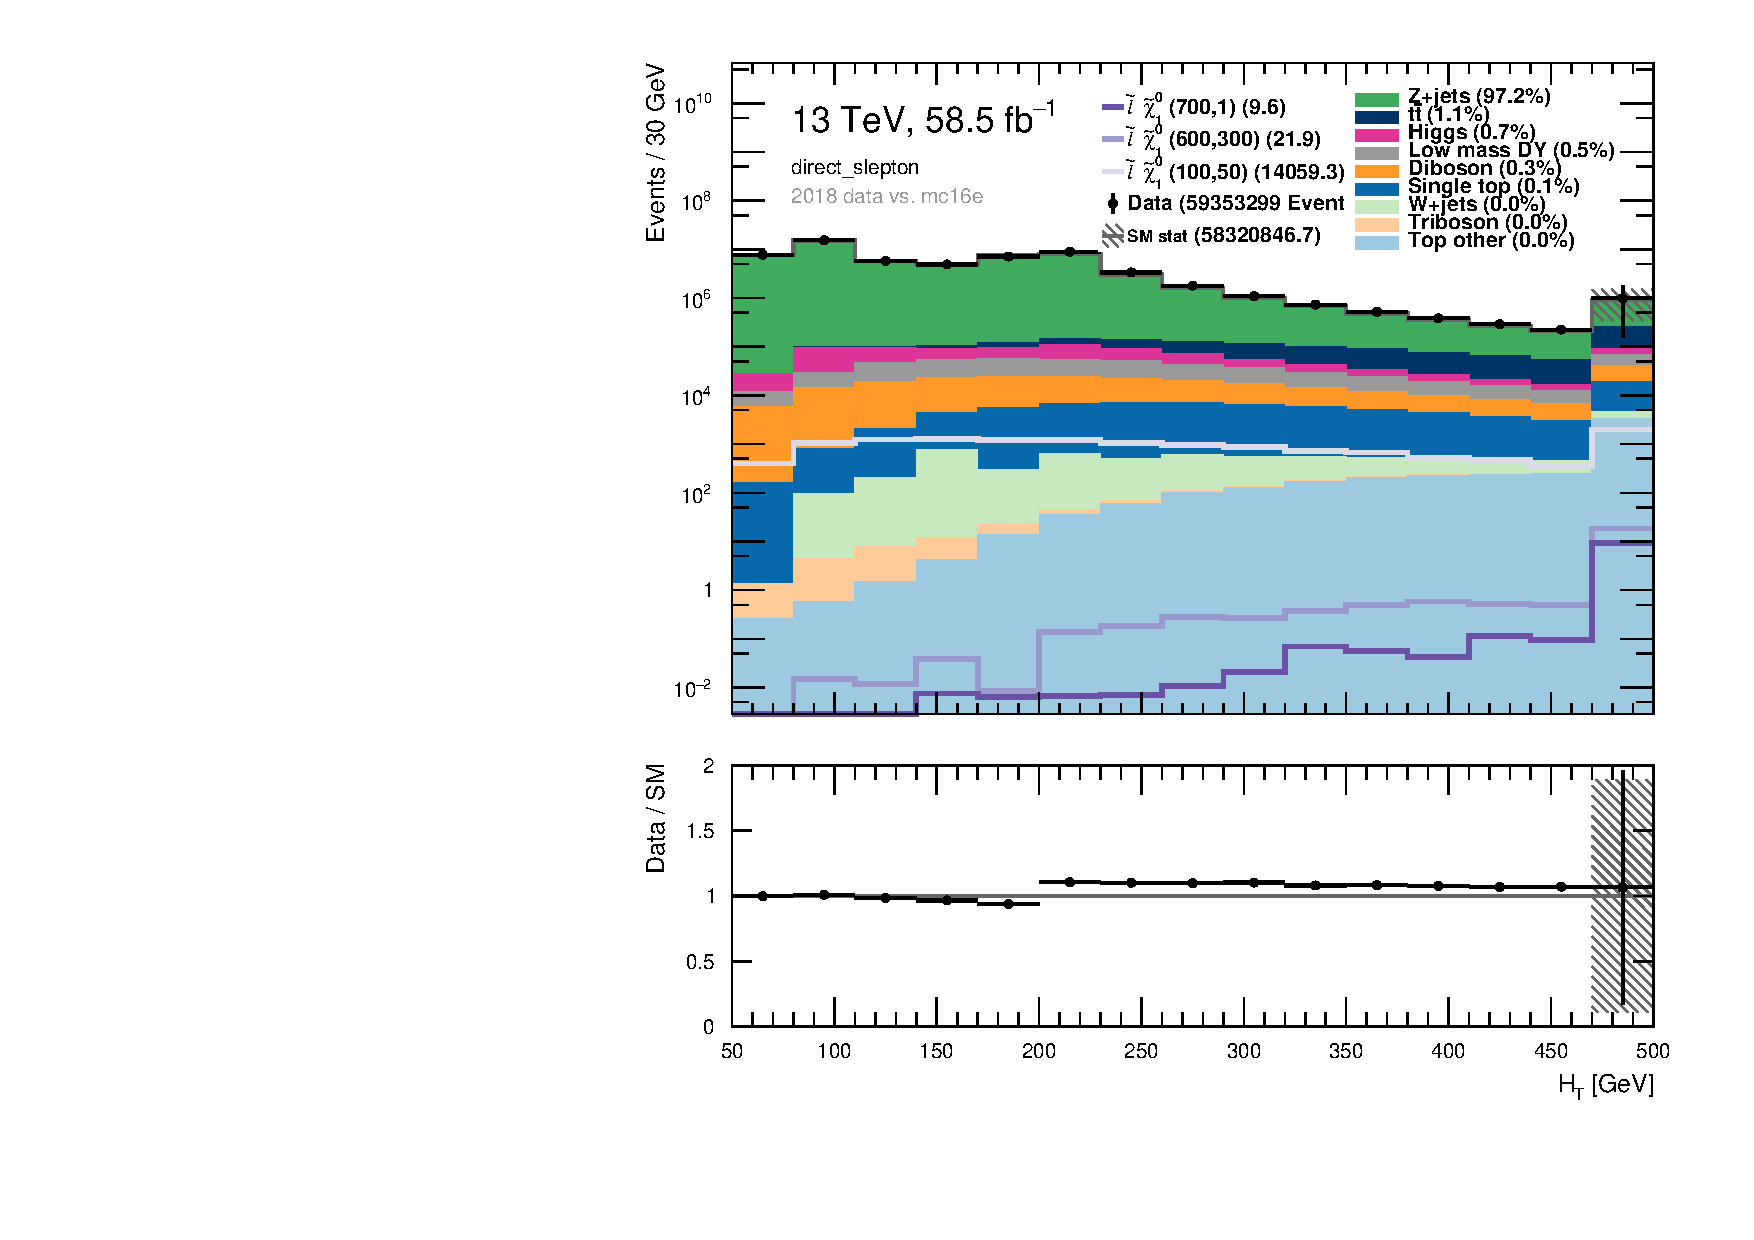
\includegraphics[width=\textwidth]{Figures/SlepSlep/CutAndCount/1stcut_2L+OS/hist1d_HT_direct_slepton.pdf}
 %   \caption{Caption}
    \label{fig:my_label}
    \end{subfigure}
%\end{adjustwidth}
\end{figure}
\end{comment}